%\documentclass[preprint]{iucr}              % DO NOT DELETE THIS LINE
\documentclass{iucr}              % DO NOT DELETE THIS LINE

\usepackage{siunitx}
\usepackage{color}
% \usepackage{amsmath,amssymb}
\usepackage{amsfonts} 
\usepackage{mathtools}
\usepackage[normalem]{ulem}

% rotation table labels...
% see https://tex.stackexchange.com/questions/98388/how-to-make-table-with-rotated-table-headers-in-latex
\usepackage{adjustbox}
\usepackage{array}
\usepackage{booktabs}
\usepackage{multirow}
\usepackage{enumitem}

\newcommand{\todo}[1]{{\color{red}[TODO: "#1'']}}
\newcommand{\inblue}[1]{{\color{blue}#1}}
\newcommand{\inred}[1]{{\color{red}#1}}
\newcommand{\ingreen}[1]{{\color{green}#1}}
\newcommand{\soutred}[1]{{\color{red}\sout{#1}}}
\newcommand{\lambdabar}{{\mkern0.75mu\mathchar '26\mkern -8.2mu\lambda}}

\definecolor{JSR_blue}{RGB}{51, 102, 154}
\newcommand{\jsrblue}[1]{\textcolor{JSR_blue}{#1}}

\newcolumntype{R}[2]{%
    >{\adjustbox{angle=#1,lap=\width-(#2)}\bgroup}%
    l%
    <{\egroup}%
}
\newcommand*\rot{\multicolumn{1}{R{90}{1em}}
%
}
\journalcode{S}


\begin{document}                  % DO NOT DELETE THIS LINE

% \title{Focusing partially-coherent x-ray beams with lenses. Multi-optics simulations}
\title{A fast and light tool-set for partially-coherent beamline simulations in 4$^{\text{th}}$ generation storage rings based on coherent mode decomposition}

\cauthor[]{\jsrblue{Manuel}}{\jsrblue{Sanchez del Rio}}{srio@esrf.eu}{address if different from \aff}
\author[]{\jsrblue{Rafael}}{\jsrblue{Celestre}}
\author[]{\jsrblue{Juan}}{\jsrblue{Reyes-Herrera}}
\author[]{\newline \jsrblue{Philipp}}{\jsrblue{Brumund}}
\author[]{\jsrblue{Marco}}{\jsrblue{Cammarata}}

\aff[]{ESRF - The European Synchrotron, 71 Avenue des Martyrs, 38000 Grenoble, \country{France}}

\maketitle                        % DO NOT DELETE THIS LINE

% -----------------------------------------------------------------
% -----------------------------------------------------------------

\begin{synopsis}
Simulations of focusing partial coherent beams with x-ray lenses are performed with different software packages (ShadowOui, SRW, COMSYYL and WOFRY). The four codes give comparable results, that are discussed in detail. 
\end{synopsis}

% -----------------------------------------------------------------
% -----------------------------------------------------------------

\begin{abstract}
We simulate the focusing of the radiation produced by fourth-generation storage rings. We present a new algorithm to perform coherent mode decomposition of the undulator radiation requiring low computer resources, like a common laptop. It is based in reducing the problem to treat one-dimension wavefronts. The validity of this approximation is discussed, and its results are compared against multiple optics packages implementing a variety of methods for dealing with partial coherence: full 2D coherent mode decomposition, Monte-Carlo combination of wavefronts from electrons entering the undulator with different initial conditions, and hybrid ray-tracing hybrid correcting geometrical optics with wave optics. The new code gives comparable results to the other codes for an undulator and four different setups of an optical system composed by a slit and two transfocators.
\end{abstract}

% -----------------------------------------------------------------
% -----------------------------------------------------------------
\section{Introduction}
\label{sec:introduction}
% -----------------------------------------------------------------
% -----------------------------------------------------------------

The migration to fourth-generation storage-rings has significantly improved brilliance and coherence of the X-ray synchrotron sources. This has a beneficial impact for many applications requiring coherent beams, such as X-ray photon correlation spectroscopy, coherent diffraction imaging, propagation-based phase-contrast imaging, and ptychography.
%(see, e.g. \cite{paganin_book}). 
The transversal coherence fraction of the new sources is increased by at least one order of magnitude with respect the 3$^{\text{rd}}$ generation sources (typically from 10$^{-3}$ to 10$^{-2}$ at 10 keV). A small pinhole was necessary with 3$^{\text{rd}}$ generation sources to gain coherence, with a dramatic loss of flux. Instead, at 4$^{\text{th}}$ generation sources, a slit with much higher transmittance is used to improve and tune the coherent fraction of the beam. 

The diffraction effects produced by the interaction of the beam with the boundaries and surface of the optical elements strongly affect the quality of the beam. Its accurate modeling is fundamental for the design and optimization of beamlines at 4$^{\text{th}}$ generation sources. The physical models for the limiting cases of full incoherence (usually simulated by geometrical ray-tracing) or by propagating a single wavefront (valid for fully coherent radiation) are not sufficient for a complete understanding of the beam transport. Indeed, the coherent fraction of the radiation emitted by new generation storage rings, although much improved with respect to previous generations, is still of the order of a few per cent at hard X-rays. This means that partial coherence should be taken into account. In the last years several approaches have demonstrated to work for beamlines using undulator radiation. Starting from incoherent beams, \citeasnoun{codeHYBRID} proposed some correction algorithms to include diffraction effects that happen with coherent radiation. More accurate methodologies exploit the well-known propagation of coherent wavefronts. The partial coherence is treated by propagating a set of wavefronts that all together describe the undulator radiation. Two approaches are possible. One consists in calculating the wavefronts emitted by electrons entering in the undulator with different initial conditions, sampled by Monte Carlo from the electron beam emittance (multi-electron in SRW) \cite{codeSRW_ME}. A second method assigns these wavefronts to the coherent modes, that are eigenfunctions of the cross-spectral density (CSD), and are calculated numerically by making a coherent mode decomposition (CMD) of the undulator source \cite{codeCOMSYL}.  


In this paper we propose a new method for dealing with partial coherence of undulator beams. The key point is to reduce the dimensionality of the problem to deal with 1D wavefronts (i.e. separating horizontal and vertical directions). A full treatment of coherent mode decomposition with 2D wavefronts was implemented a few years ago in the COMSYL package \cite{glass2017}. This method requires the use of high-performance computer (HPC) clusters, facilities that are not always at a hand. The problem is to manipulate and diagonalize a huge stack representing the CSD, that is a 4D entity when using 2D wavefronts. Since then, different techniques have been applied to deal with the magnitude of the problem, for example using Single-Value-Decomposition for diagonalization \cite{SVDHanXu}, or analytical treatment of the quadratic phase \cite{ChubarCMD2022}, but none of them get rid of using HPC. In this paper we demonstrate that whenever the 1D simplification can be used, in many cases so far, the results of this new method are comparable to the other methods but with gaining many orders of magnitude in computer resources, thus allowing simulations in a simple laptop. 

The new code is benchmarked against other existing codes that are available in OASYS \cite{codeOASYS}  simulation ecosystem. The optical system used derives from the project for the new ID18 beamline at the upgraded EBS-ESRF storage ring. We have compared results for different setups implementing two refractive systems (transfocators), plus a slit placed upstream from the transfocators. The focal spots produced by four different transfocator configuratiuons are studied in detail using four packages: i) the novel 1D CMD, implemented in the code WOFRY1D, ii) full CMD in 2D with COMSYL \cite{codeCOMSYL}, iii) multi-electron simulations as implemented in SRW \cite{codeSRW}, and iv) hybrid ray-tracing as described by \citeasnoun{codeHYBRID} and implemented in ShadowOUI \cite{codeSHADOWOUI}.

% To study the performances of such systems a new algorithm for coherent mode decomposition (CMD) of the undulator beams has been developed. This method is very fast allowing parametric simulations in a common laptop.

% The high efficiency of the CMD software developed is obtained by implementing a 1D model, therefore studying separately the horizontal and vertical planes. 

% Simulation of the source include coherent mode decomposition (CMD) using COMSYL \cite{codeCOMSYL}, or Monte-Carlo multi-electron propagation with SRW \cite{codeSRW}. It is also found that ray-tracing simulations using the ``hybrid" method \cite{codeHYBRID} give good approximations to the correct results for these systems. A simplified algorithm for CMD in 1D is available in WOFRY. It is very fast allowing parametric simulations in a common laptop, with results in good agreement with the other methods that require a computing cluster.

% The paper is organized as follows. Section~\ref{sec:theory} summarizes the methodology used for 1D coherent mode decomposition of undulator beams and their transport along the beamline. Section~\ref{sec:onelens} analyzes the focusing of partially-coherent beams with a single refractive system (lens). Section~\ref{sec:twolenses} discusses the pairing of two refractive systems. Section~\ref{sec:complete-beamline} shows simulations for the full beamline and compares different methodologies for a selected case. We finish with a general discussion in Section~\ref{sec:discussion} and  concluding remarks in Section~\ref{sec:summary}. 

% -----------------------------------------------------------------
% -----------------------------------------------------------------
\section{Methods for describing partial coherent beams from undulators in a storage ring}\label{sec:part_coh}
% -----------------------------------------------------------------
% -----------------------------------------------------------------
 \newline
% In this section we present four methods used for dealing with partially-coherent x-ray beams emitted by undulators in low-emittance storage rings. Three of those are already-established methods:  hybrid ray-tracing in ShadowOUI; Monte Carlo multi-electron simulations as implemented in SRW; and the 2D-CDM method implemented in COMSYL. Despite being independently maintained and distributed projects, these are conveniently grouped together within the OASYS suit \cite{codeOASYS} and hence their choice for benchmarking. The fourth approach is the proposed 1D-CMD method separating the horizontal- and vertical-directions implemented in WOFRY, which is also featured in OASYS.

In this section we present the basic theory underneath the numeric calculations with the packages used. We start showing how the partial coherence appears when a bunch of electrons travel along the insertion device. Although a single electron emit coherent radiation, a beam of electrons emit partial coherent light: high coherence is associated with low emittance. 

% four methods used for dealing with partially-coherent x-ray beams emitted by undulators in low-emittance storage rings. Three of those are already-established methods: Monte Carlo multi-electron simulations as implemented in SRW; the 2D-CDM method implemented in COMSYL; and the hybrid ray-tracing in ShadowOUI. Despite being independently maintained and distributed projects, these are conveniently grouped together within the OASYS suit \cite{codeOASYS} and hence their choice for benchmarking. The fourth approach is the proposed 1D-CMD method separating the horizontal- and vertical-directions implemented in WOFRY, which is also featured in OASYS.

% -----------------------------------------------------------------
\subsection{Description of undulator emission}
\label{sec:undulator}
% -----------------------------------------------------------------

We quickly remind that an ultrarelativistic particle following a curved trajectory (usually wavy as produced by alternated magnetic fields in insertion devices) emit radiation, which electric field can be calculated in the framework of the classical electrodynamics (see e.g. \cite{jackson}). The electric field at an observation point $\textbf{r}=(x,y,z)$ at a given photon frequency $\omega$ can be written as: 

\begin{equation}
\label{eq:undulator}
    E_{\omega}(\textbf{r}) = \frac{i e \omega}{4 \p e \epsilon_0} 
    \int_{-\infty}^{\infty}
    \left[ 
    \frac{
    \textbf{n} \times [(\textbf{n} - \mathbf{\beta}) \times \dot{\mathbf{\beta}}]
    }
    {
    (1- \mathbf{\beta} . \textbf{n})^\inred{2}
    } +  
    \frac{c}{\gamma^2 R}   \frac{\textbf{n} - \mathbf{\beta}}{(1-\mathbf{\beta} . \textbf{n})^3} 
    \right] \exp^{i \omega (t - \textbf{n}\mathbf{\beta}} dt
\end{equation}
where $e$ is the electron charge, $c$ the velocity of light, $\epsilon_0$ the electric constant,
$\textbf{n}(t)=\textbf{R}-\textbf{r}_{\textbf{e}}(t)/|\textbf{R}-\textbf{s}_{\textbf{e}}(t)|$ is the unit vector
pointing from the particle to the observation point $\textbf{R}$; $\textbf{r}_{\textbf{e}}(t)$ is the
electron trajectory of the reference electron and the dot denotes the time derivative.

% where the retarded time $t'$ verifies $t=t'+R(t')$. 
This equation permits to calculate the wavefront at a given frequency and at a given plane of coordinates $(x,y)$ distant $z_0$ from the origin ($\textbf{r}=(x,y,z_0)$). The origin is usually set at the center of the ID. Full transversal coherence is obtained as $E_{\omega}$ is unique and well-defined (amplitude and phase) in space.

The case discussed is for a single electron, but if $N_e$ electrons follow the same trajectory at the same time (an illusion that the electrons overlap in space) the intensity is $N_e$ times those obtained from equation (\ref{eq:undulator}). This is called "filament beam", it is useful to represent an idealized zero-emittance ring, and also radiates a fully transverse coherent wavefront.

Several codes are available in the synchrotron community to calculate the undulator emission characteristics in different cases. The codes URGENT \cite{codeURGENT} and US \cire{codeUS} compute undulator emission in the far-field for undulators with sinusoidal magnetic field. The codes SPECTRA \cite{codeSPECTRA} and SRW \cite{codeSRW} are generic. They calculate emission in the near and far-field for any electron trajectory (with different initial conditions) and submitted to an arbitrary magnetic field \cite{Chubar1995}.

% -----------------------------------------------------------------
\subsection{Electron beam distribution in storage rings}
\label{sec:electronbeam}
% -----------------------------------------------------------------


The electron trajectory previously used $\textbf{r}_{\textbf{e}}(t)$ is completely determined by the map of the magnetic field of the ID and the initial conditions at the entrance of the ID. 
At any position of the storage ring, usually designed by $s$, a single electron can be described by 5 coordinates:
$\textbf{S}= (x_\text{e},y_\text{e},  x'_\text{e},y'_\text{e},\delta)$ representing the phase space coordinates and a term $\delta$ expressing the relative deviation of the electron energy from main storage ring energy. 

From the accelerator physics, at a given position $s$ of the storage ring, the many-electrons in a bunch follow a 5D Gaussian distribution

\begin{equation}\label{eq:f-electrons}
f(\textbf{S}) = \frac{1}{(2 \pi)^{5/2} \sqrt{\text{det}(M^{-1})}} \exp
        \left( -\frac{1}{2} \textbf{S}^T M \textbf{S} \right),
\end{equation}
with $M$ the 5$\times$5 is the inverse of the generalized variance matrix. If the variables are uncorrelated, only the diagonal terms are non-zero and are ($1/\sigma_x^2,1/\sigma_y^2,1/\sigma_{x'}^2,1/\sigma_{y'}^2,1/\delta^2)$. 

We can also considere that the elecrons packed in a bunch have also Gaussian distribution with $\sigma_x$ in the longitudinal direction. 
\todo{discuss longitudinal direction $\sigma_z$?}

% $f(\textbf{S})$. , with given r.m.s spatial ($\sigma_x$, $\sigma_y$, $\sigma_z$), angular ($\sigma_{x'}$,$\sigma_{y'}$), and energy $\delta$ values. Correlation terms are, in general, different from zero only for the horizontal ($\sigma_{x x'}$) and vertical ($\sigma_{y y'}$). 
 

% -----------------------------------------------------------------
\subsection{Emission from electron bunches}
% -----------------------------------------------------------------

Having summarized the coherent emission from a single electron in section \ref{sec:undulator} and how the electrons are statistically distributed in a bunch (section \ref{sec:electronbeam}), we want to put them together to obtain the light emission from the electron bunch.

The total electric field emitted from all electrons in a bunch is
\begin{equation}
    E_{\omega \text{~bunch}}(\textbf{r}) = \sum_{i=1}^{N_e} E_{\omega,i}(\textbf{r}).
\end{equation}

In terms of intensity, and using the electron distribution, an expression for the emission from the bunch of $N_\text{e}$ electrons circulating in a storage ring is given by: 
\begin{equation}
\begin{split}
|E&_{\omega\text{~bunch}}(\textbf{r})|^2 \approx \\
 &N_\text{e} \int\big| E_\omega(\textbf{r};\textbf{S}_\text{e},s_0)\big|^2 f(\textbf{S}_\text{e})~ d\textbf{S}_\text{e}~+\\
&+~ N_\text{e}(N_\text{e}-1)\bigg| \int E_\omega(\textbf{r};\textbf{S}_\text{e}, s_0) f(\textbf{S}_\text{e})~ d\textbf{S}_\text{e} \bigg|^2.
\end{split}
\label{eq:SR}
\end{equation}
Note that $E_\omega(\textbf{r};\textbf{S}_\text{e}, s_0)$ is the emission at the observation point $\textbf{r}$ by a single electron that makes a trajectory defined by the undulator magnetic field and electron initial conditions $(\textbf{S}_{\text{e}}, s_0})$
The first term is a sum of the intensity $|E_{\omega}|^2$ at $\textbf{r}$ of every electron weighted its probability $f$. The second term stands for the enhancement of the intensity due to coherent superposition of the emission of the $N_e$ electrons. This term not zero for electrons closely packed, typically when $\sigma_z < \lambda$ ($\lambda$ is the photon wavelength).  In other words,    
the first term in the sum from Eq.~\ref{eq:SR} describes temporally incoherent SR and the second term models temporally coherent SR: $\text{I}_\text{~bunch} = \text{I}_\text{~iSR}+\text{I}_\text{~cSR}$. For emitted wavelengths shorter than the electron bunch length, the power associated with the term $\text{I}_\text{~cSR}$ vanishes quickly \cite{CSR,Wiedemann2015}.
Considering typical undulator radiation emission, i.e. x-ray energy ranges from a few hundred electron-volts to a few hundred keV, and typical electron bunch lengths in storage rings ($\sigma_{T}>30$~ps), $\text{I}_\text{~cSR}$ can be neglected when considering standard monochromatisation schemes in beamlines. \todo{ I WOULD REMOVE THIS: A further simplification to Eq.~\ref{eq:SR} is done when considering that the intensity of the single-electron emission is not dependent on the initial electron position $z_\text{e}$. The integration of Eq.~\ref{eq:SR} can then be done in 5 dimensions.}


\todo{MOVE TO SRW OR REMOVE?

Equation~\ref{eq:SR} can be expressed in number of photons ($\text{d}N_{ph}$) per unity of time ($\text{d}t$) per unit surface ($\text{d}S$) per per unit relative bandwidth ($\text{d}\omega\big/\omega$) by:
\begin{equation}
\frac{\text{d}N_{ph}}{\text{d}t~\text{d}S~\text{d}\omega\big/\omega}=\frac{c^2\alpha \text{I}_\text{~bunch}}{4\pi^2e^3N_e}|E_{\omega\text{~bunch}}(\textbf{r})|^2,
\label{eq:SR_ph}
\end{equation}
where\footnote{See also the works by \citeasnoun{kim1995} and \citeasnoun{hulbert1992}.} $c$ is the speed of light, $\alpha$ is the fine-structure constant, $\text{I}_\text{~bunch}$ is the storage ring current and $e$ is the electron charge \cite{Chubar1995}.
}

In a similar way, the mutual correlation of the electric field between two observation points $\textbf{r}_1$ and $\textbf{r}_2$ is
\begin{equation}\label{eq:CSDallaChubar}
\begin{split}
      &\big\langle E^*_{\omega}(\textbf{r}_1)  E_{\omega}(\textbf{r}_2)\big\rangle = 
      \sum_{i=1}^{N_e} \sum_{j=1}^{N_e} E^*_{\omega,i}(\textbf{r}_1) E_{\omega,j}(\textbf{r}_2) = \\
      & N_e^\inred{2}\int \int 
      E^*_{\omega}(\textbf{r}_1;\textbf{S}_{\textbf{e},1},s_0)
      E_{\omega}(\textbf{r}_2;\textbf{S}_{\textbf{e},2},s_0)
      f(\textbf{S}_1) f(\textbf{S}_2)
      d\textbf{S}_{\textbf{e},1} d\textbf{S}_{\textbf{e},2}.
\end{split}
\end{equation}
where $\bullet^*$ indicates the complex conjugate, the brackets $\langle \bullet \rangle$ indicate sum over the bunches, $\textbf{r}_1=(x_1,y_1,z_1)$ and $\textbf{r}_2=(x_2,y_2,z_2)$. This equation is the cross-spectral density, that will be discussed later and rewritten in more manageable form. 

% This implies necessarily some mathematical tools, probably using convolution. 
% Indeed, Kwang-Je Kim developed a propagation theory of synchrotron radiation using Wigner distribution \cite{KimConvolution}. He introduced the ``brightness convolution theorem" stating that the source brightness due to a collection of electrons randomly distributed in their phase space is calculated by a convolution of the source brightness due to a reference electron with the electron distribution function. 



% where $E_{\omega\text{~bunch}}(\textbf{r})\equiv E_{\text{~bunch}}(x,y, z;\omega)$ is the resulting bunch emission; $E_\omega(\textbf{r})\equiv E(x,y, z;\omega)$ is the single-electron emission; 
% $\textbf{s}_\text{e}=(x_\text{e},y_\text{e},z_\text{e})$ represents the electrons initial positions,

% $\textbf{s}'_\text{e}=(x'_\text{e},y'_\text{e})$ gives the electrons initial directions and $\gamma_\text{e}$ is the electron-beam energy subjected to the energy spread $\delta \gamma_\text{e}$. These variables are uncorrelated and have Gaussian distribution in a 6-dimensional space \cite{codeSRW_CSR}. 

% The single-electron emission $E_\omega(\textbf{r})$ is, by definition, fully coherent\footnote{A similar abstraction is the zero-emittance or filament beam, that also radiates a fully transverse coherent wavefront, but with an intensity proportional to $N_e$.}. 




% -----------------------------------------------------------------
\subsection{Multi-electron Monte Carlo (SRW-ME)}
% -----------------------------------------------------------------

Synchrotron radiation emitted by undulators in storage rings is a fundamentally random process and should be treated probabilistic. The SRW-ME algorithm used to account for partial coherence implements Eq.~\ref{eq:SR} by individually calculating the SR emission of several electrons subjected to the initial conditions sampled from $f(\textbf{s}_\text{e}, \textbf{s}'_\text{e}, \gamma_\text{e})$ assuming these are uncorrelated and passing through an arbitrary magnetic field describing the x-ray source. Each resulting electric field from this Monte-Carlo sampling is then propagated through the beamline until the observation point, where the contributions from different electrons are added in intensity \cite{codeSRW_ME}. It is impractical (and unnecessary) to account for the emission of every single electron in a beam that very often has a current of few hundreds mA. Electrons are then divided in so-called macro-electrons (\textit{me's}), which is an abstraction that allows to group the emission of several individual electrons into one ``superparticle'' emitting a fully-coherent wavefront but with resulting intensity given by the total intensity $\text{I}_\text{~bunch}$ divided by the number of macro-electrons $N_{me's}$ used in the simulation:
\begin{equation}
% \begin{split}
|E_{\omega\text{~bunch}}(\textbf{r})|^2 \approx \frac{N_e}{N_{me's}}\sum_{n=0}^{N_{me's} - 1}\big| E_\omega(\textbf{r};\textbf{s}_{\text{e}_n}, \textbf{s}'_{\text{e}_n}, \gamma_{\text{e}_n})\big|^2.
% \end{split}
\label{eq:SR_SRW}
\end{equation}
An advantage of the SRW-ME approach is that the electric fields of the \textit{me's} propagate independently from each other, which allows a convenient parallelisation of the wavefront propagations among many processors. Indeed, SRW-ME calculations require the use of HPC in most cases.

% -----------------------------------------------------------------
\subsection{Coherent mode decomposition of undulator radiation}\label{sec:CMD}
% -----------------------------------------------------------------

The cross-spectral density
\begin{equation}
W_\text{2D}(\textbf{r}_1,\textbf{r}_2;\omega) = \big\langle E^*_{\omega}(\textbf{r}_1)  E_{\omega}(\textbf{r}_2)\big\rangle
\label{eq:CSD_2D}
\end{equation}
expresses the correlation of the emitted radiation between any two spatial points $\textbf{r}_1$ and $\textbf{r}_2$. It is the fundamental object that we will use to describe all partial coherence properties of the synchrotron beams. It completely describes and quantified the ``partial coherence" of these beams. We justify first, in the context of existing literature, the conditions of its usage for synchrotron light. Then we present the CMD and its practical implementation in 2D (with COMSYL) and the new 1D algorithm (with WOFRY1D).   


% -----------------------------------------------------------------
\subsubsection{Validity of CSD usage for emission in storage rings}
% -----------------------------------------------------------------

\citeasnoun{geloni2008} show that although SR emission (a random process obeying Gaussian statistics) is not intrinsically stationary nor homogeneous, second order coherence theory of scalar fields as presented by \citeasnoun{mandel_wolf} can be applied if the following conditions are observed:
\begin{enumerate}[label=(\roman*)]
\item radiation frequency $\omega$ is ``sufficiently high";
\item $e^-$ bunch length $\sigma_{T}$ ``sufficiently large" so that $\omega\sigma_{T}\gg1$;
\item radiation bandwidth $\Delta_\omega$ is not ``too narrow" ($\Delta_\omega\gg1/\sigma_{T}$).
\end{enumerate}
Basically excluding infra-red downwards, condition (i) holds for soft- to hard x-rays, which are upwards in frequency; condition (ii) is satisfied by storage rings, where typically $\sigma_{T}>30$~ps, but not at free-electron lasers, where $\sigma_{T}<0.1$~ps due to micro-bunching effects; and finally, condition (iii) is generally met by standard\footnote{\citeasnoun{geloni2008} provide a counter-example in Ref[15] ibid.} monochromatisation schemes. This set of conditions ensures that SR emission is a quasi-stationary (or a wide-sense stationary) process. The conditions for considering undulator radiation quasi-homogeneous are implicitly met when:
\begin{enumerate}[label=(\roman*)]
\setcounter{enumi}{3}
\item $N_\text{x}\gg1$ and $D_\text{x}\gg1$;
\item $N_\text{y}\gg1$ and/or $D_\text{y}\gg1$,
\end{enumerate}
with:
\begin{equation*}
    N_\text{x,y}=\frac{\sigma^2_\text{x,y}}{\lambdabar L_u}, \quad D_\text{x,y}=\frac{\sigma'^2_\text{x,y}}{\lambdabar/L_u}
\end{equation*}
where $\sigma_\text{x,y}$ and $\sigma'_\text{x,y}$ represent the electron beam transverse sizes and divergences, $L_u$ is the undulator length (number of periods $N_u$ times the magnetic period $\lambda_u$) and $\lambdabar=\lambda/2\pi$, with $\lambda$ the wavelength of the emitted photons. Conditions (iv) and (v) are met for the wavelengths already restricted by (i). As noted by \citeasnoun{geloni2008}, the conditions (i)-(v) are practically non-restrictive under cases of practical interest.

% -----------------------------------------------------------------
\subsubsection{Coherent modes, coherent fraction and coherent length.}
% -----------------------------------------------------------------

The CSD (equation \ref{eq:CSD_2D}) is used to define the spectral density\footnote{Which is sometimes loosely called intensity. The spectrum density and the intensity functions are equivalent for the quasi-monochromatic case. The same holds for the CSD and the mutual optical intensity (MOI) \cite{mandel_wolf}.} for the case where $\textbf{r}=\textbf{r}_1=\textbf{r}_2$ as $I_{2D}(\textbf{r};\omega)=W_\text{2D}(\textbf{r},\textbf{r};\omega)$. We also define the normalised cross-spectral density function or spectral degree of coherence (SDC):
\begin{equation}
\mu(\textbf{r}_1,\textbf{r}_2;\omega) = \frac{W_\text{2D}(\textbf{r}_1,\textbf{r}_2;\omega)}{\sqrt{I(\textbf{r}_1;\omega) I(\textbf{r}_2;\omega)}}.
\label{eq:DTC}
\end{equation}
The absolute value of Eq.~\ref{eq:DTC} is limited: $0\leq|\mu(\textbf{r}_1,\textbf{r}_2;\omega)|\leq 1$, where $|\mu|=0$ means total uncorrelation and $|\mu|=1$ denotes full correlation of the fluctuations at positions $\textbf{r}_1$ and $\textbf{r}_2$.

A well known result from coherence theory is the coherent mode representation of partially coherent fields in free-space - see §4.7.1 in \cite{mandel_wolf}. It is possible to decompose the CSD in a infinite sum of orthonormal coherent modes:
\begin{equation}\label{eq:W2DCMD}
W_\text{2D}(\textbf{r}_1,\textbf{r}_2;\omega) = \sum_{n=0}^{\infty} \Lambda_n(\omega) \Phi_{n}^*(\textbf{r}_1;\omega) \Phi_{n}(\textbf{r}_2;\omega)
\end{equation}
where $\Lambda_n$ (eigenvalues) are the intensity weights and the $\Phi$ are the coherent modes (eigenfunctions). 
Some important characteristics of this coherent mode decomposition are: 

\begin{enumerate}[label=(\roman*)]
\item the modes $\Phi$ are orthonormal in the integral sense;
% \end{enumerate}
% \begin{equation*}
% \int W_\text{2D}(\textbf{r}_1,\textbf{r}_2;\omega)  \Phi_{n}(\textbf{r}_1;\omega)~ \text{d}\textbf{r}_1 = \Lambda_n(\omega) \Phi_{n}(\textbf{r}_2;\omega);
% % \label{eq:orthonormal_modes}
% \end{equation*}
% \begin{enumerate}[label=(\roman*)]
% \setcounter{enumi}{1}
\item the modes maximize the CSD making the truncation optimal:
\end{enumerate}
\begin{equation*}
\Lambda(\omega) \in \mathbb{R}
:~0\leq \Lambda_{i+1}(\omega)<\Lambda_i(\omega);~\forall~i \in \mathbb{N};
\end{equation*}
\begin{enumerate}[label=(\roman*)]
\setcounter{enumi}{2}
\item the eigenvalues $\Lambda_n$ are a measure of the intensity of the corresponding mode $\Phi_{n}$; 
\item we define the occupation $\eta$ of the i-th mode as the normalized intensity: 
\begin{equation}
\eta_i(\omega) =\frac{\Lambda_i(\omega)}{\sum\limits_{n=0}^\infty{\Lambda_n(\omega)}};
\end{equation}
\item radiation is considered fully-coherent if and only if there is only a single mode.
\end{enumerate}

From these arguments, it is now natural to rigorously define coherent fraction ($\text{CF}_\text{2D}$) as the occupation of the first coherent mode:
\begin{equation}
\text{CF}_\text{2D}=\eta_0=\frac{\Lambda_0(\omega)}{\sum\limits_{n=0}^\infty{\Lambda_n(\omega)}}. \label{eq:CF2D}
\end{equation}
When using Eq.~\ref{eq:CF2D}, it is relevant to consider that if there is spatial filtering or any sort of beam clipping the modes $\Phi$ do not propagate retaining their orthogonality and their occupation $\eta$. In this case, a reapplication of the CMD to the cropped modes (rediagonalisation) is imperative to recalculate the new $\text{CF}_\text{2D}$.

We also define the transverse coherence length (CL) based on the width of the first mode $\Phi_0$, acknowledging issues with this definition arising mainly from the fact that here is no unanimous accepted way of defining the beam width. However, given the importance of such parameter for daily beamline operations (eg. choosing slit sizes) and that blindly applying the van-Cittert-Zernike (VCZ) theorem may lead to errors - cf. §4.1 in \cite{geloni2008}, we decided to put the CL on a firmer footing. This definition holds for both horizontal directions and is dependent on the criteria used for defining the beam width along that direction. % \todo{a possible new section describing the coherent parameters (CF, coherent length, etc) and the way to obtain them via rediagonalization...}

The interest of the coherent mode decomposition method in optical design of x-ray beamlines is manyfold: i) the possibility of propagating a partially-coherent beam along a beamline by just propagating a few hundred modes which behave like coherent wavefronts as opposed to a few thousand wavefronts when doing multi-electron Monte-Carlo simulations; ii) the use of the coherent fraction (a scalar parameter) as a well-defined measure of how coherent is the beam at any position of the beamline; iii) the numerical storage of the $N_m$ modes that depend on two spatial variables is more economic than the storage of the cross-spectral density $W$ that depends on four variables; and iv) the infinite series converges smoothly to the CSD, therefore the truncation at a limited number of modes $N_m$ always guarantees that it is the best possible reduced representation of the CSD and can be quantified (usually $N_m$ is chosen to get the 99\% of the spectral density). 

% -----------------------------------------------------------------
\subsubsection{Coherent mode decomposition with COMSYL} 
% -----------------------------------------------------------------

COMSYL (COherent Modes for Synchrotron Light) \cite{codeCOMSYL} is a software package to perform CMD of the emission of an undulator in an storage ring. Its main characteristics are summarized here. A full description of COMSYL is in \cite{glassThesis}. Applications of CMD using COMSYL for beamlines at the ESRF-EBS are in \cite{glass2017, hierarchical}. 


Coherent mode decomposition consists in calculating in calculating $\Lammda_i$ and $\Phi_i$ in equation \ref{eq:W2DCMD}. It can be seen as a diagonalization of $W_{2D}$ where the eigenfunctions are the coherent modes ($\Phi_i$) and the eigenvalues their intensity weights ($\Lambda_i$). They are the solution of the homogeneous Fredholm integral equation of second kind:

\begin{equation}\label{fredholm_equation}
\int d\textbf{r}_1 W_{2D}(\textbf{r}_1,\textbf{r}_2;\omega)
\Phi_i(\textbf{r}_1;\omega) = \Lambda_i(\omega) \Phi_i(\omega)
\end{equation}
The eigenvalue problem and may be rewritten as:
\begin{equation}
A_{W_{2D}}[\Phi_i] = \Lambda_i \Phi_i
\end{equation}
where we defined the Hermitian operator
\begin{equation}
A_{W_{2D}}[f]\textbf{r}  = \int d\textbf{r}' W_{2D}(\textbf{r}',\textbf{r};\omega) f(\textbf{r}').
\end{equation}

We need a recipe to calculate $W_{2D}$. 
A first look at the CSD expression (see equation \ref{eq:CSDallaChubar}) is enough to get an impression of the difficulty to compute and the huge volume it represents, because it is a 6D function. For synchrotron beams it is useful to decouple the third coordinate $z$ (position at the beamline) so $W_2D$ reduces to 4D. Knowing the CSD at a given position $z_a$ ($W_{2D}(x_1,y_1,x_2,y_2; \omega, z_a)$) it is possible (although not simple) to propagate it to another position $z_b$ and even at the origin $z=0$ (the source position).

Kwang-Je Kim developed a propagation theory of synchrotron radiation using Wigner distribution \cite{KimConvolution}. He introduced the ``brightness convolution theorem" stating that the source brightness due to a collection of electrons randomly distributed in their phase space is calculated by a convolution of the source brightness due to a reference electron with the electron distribution function. 
The Kim's brightness convolution theorem is applied in a plane $(x,y)$ where the electrons enter in the undulator at $z_e$ ($z_e=-L_u/2)$ when the origin is the center of the ID) (equation 3.37 in \cite{glassThesis}):
\begin{equation}\label{eq:comsyl_W2D}
\begin{split}
    W_\text{2D}&(\textbf{r}_1,\textbf{r}_2;\omega) = \\
    &\int d \delta d\textbf{r}
    E_\omega^*(\textbf{r}_1-\textbf{r};\omega)
    E_\omega(\textbf{r}_2-\textbf{r};\omega)
    F(\textbf{r}, \Delra\textbf{r})
\end{split}
\end{equation}
with $\mathbf{\Delta}\textbf{r}=\textbf{r}_2-\textbf{r}$, 
\begin{equation}
F(\textbf{r},\mathbf{\Delta}\textbf{r}) = \int d\textbf{r}' f(\textbf{r},\textbf{r'},\delta) \exp(i k \textbf{r}'\mathbf{\Delta}\textbf{r}),
\end{equation}
and $f$ the 5D distribution of the electrons (equation \ref{eq:f-electrons}).
% (see equation 3.39 in \cite{glassThesis})
Note that this is a 4D function as the third coordinate is fixed to $z_e$, so  now $\textbf{r}=(x,y)$ and $\textbf{r}'=(x',y')$. 
$E_\omega$ is calculates using SRW in an arbitrary plane ($z_D$) and then backpropagated to $z_e$ with a Fresnel standard SRW propagator (see below). 


COMSYL starts with a matrix method that discretizes the cross spectral density operator $A_{W_{2D}}$ in a step function basis set (equation. 4.4 in \cite{glassThesis}). The discretization is followed by an iterative diagonalization using SLEPc \cite{SLEPc}. The implementation is parallel requiring HPC. The key point of COMSYL is to avoid storing the full representing matrix, because it requires a lot of memory and computational resources. It scales essentially with $N_x^2 \times N_y$^2$ where $N_x$ and $N_y$ are the numbers of grid points in the $x$ and $y$ dimension, respectively. Typical sizes for $N_x$ and $N_y$ can easily reach a few hundred up to a few thousand. In the latter case the memory requirements would reach several thousand terabytes. To reduce the memory requirements of the matrix method COMSYL uses a two-step method that first performs a coherent mode decomposition for a zero divergence electron beam and based on this decomposition performs a second decomposition that takes the divergence into account. The memory requirement for our undulator applications is drastically reduced to about $4 N_x N_y N_m$ where $N_m$ is the number of requested coherent modes. This allows the calculation of higher harmonics or higher emittance rings where $N_x N_y \gg N_m$. 

COMSYL can be used in the OASYS environment for propagating modes along the beamline, using SRW or WORFY \todo{link to chapter 3}. 

The propagated modes $\Phi'_i$ can be used to compute the (propagated) spectral density and cross-spectral density at any point of the beamline. 
In general, the propagated wavefronts $\Phi'_i$ are not anymore coherence modes. They were modified at the optical elements (truncation, absorption) lossing the properties of orthonormality. A new CMD must be done to calculate new eigenvalues and eigenfunctions (modes) and retrieve the propagated CF. The propagated wavefronts keep orthonormality only in the cases of free propagation and ideal focusing. Any element that crop the beam or include absorption imply that $\Phi'_i$ are not longer orthonormal. 
Thus, for computing the CF at a given point of the beamline, it is necessary to perform a new CMD with the propagated CSD. It can be similar to the initial decomposition, create the representing matrix in the stepfunction basis. However, COMSYL implements
the action of the integral operator directly in terms of the coherent modes, which is much more economic in terms of
memory. 


\inred{Question to @Manolo: talk about other codes that do CMD for X-ray simulations? xrt, MOI, SRW-CMD?

Manolo's answer: Yes if they effectively do CMD on undulators: I think SRW-CMD and \cite{SVDHanXu} do that. I cited them before, stressing that they do not solve the problem of using HPC. We cannot say much about them as we do not have experience with them... MOI uses Gaussian-Shell model (not cited).  We should check again XRT and TANAKA...}

% -----------------------------------------------------------------
\subsubsection{1D coherent mode decomposition: separate horizontal and vertical directions (WOFRY)\\}
% -----------------------------------------------------------------

We now suppose that the CSD (Eq.~\ref{eq:CSD_2D}) can be written as a product of a horizontal- and a vertical cross-spectral densities: 
\begin{equation}
W_\text{2D}(\textbf{r}_1,\textbf{r}_2;\omega) = W_\text{1D}(x_1,x_2;\omega)W_\text{1D}(y_1,y_2;\omega).
\label{eq:CSD_2D_bis}
\end{equation}
% \begin{equation}
% W_\text{2D}(\textbf{r}_1,\textbf{r}_2;\omega) = W_\text{1D}(x_1,0,x_2,0;\omega)W_\text{1D}(0,y_1,0,y_2;\omega).
% \label{eq:CSD_2D_bis2}
% \end{equation}
The factorisation in Eq.~\ref{eq:CSD_2D_bis} has been discussed §3.1 from \cite{geloni2008} - see Eq.~56 ibid; this rearranging of Eq.~\ref{eq:CSD_2D} is only valid for quasi-homogeneous sources, that is, when the intensity distribution in the source is a slowly varying function compared to the coherence length. In the context of the Wigner distribution, this separation in horizontal and vertical components has been discussed by various authors is believed to work well for photon energies not far from the undulator resonance and for non-round beams \cite{tanaka2014,nash2021}. The CSD and the Wigner distribution being related by a Fourier transform. 

 The CMD for each direction is:
\begin{equation}
W(x_1,x_2;\omega) = \sum_{n=0}^{\infty} \lambda_n(\omega) \phi_n^*(x_1;\omega) \phi_n(x_2;\omega) 
\label{eq:CMD1D}
\end{equation}
with $\lambda_n$ the 1D eigenvalues and $\phi_n$ the 1D eigenfunctions. This gives raise to two values of coherence fraction, for the horizontal and vertical directions, and the 2D CF is the product CF$_{2D}$=CF$_H \times$ CF$_V$.

This separation results in a CSD that is now a 2D function. Therefore it is very easy to store, manipulate and disgonalize using common tools, like the numpy library. It can be built with the same recipe as in COMSYL: calculate the 1D emission at a given plane (we use now pySRU \cite{codePSU}), propagate it back to the source plane (using zoom propagator, see below), and combine them using the Kim's brightness convolution theorem, that for a 2D CSD is effectively constructed using equation 3.51 in \cite{glass2017}.

This recipe is implemented in the WOFRY wavefront propagation package in OASYS. For a typical beamline, two calculations are done: one for the horizontal direction and another for the vertical. These two results are when combined: as mentioned, CF$_{2D}$=CF$_H \times$ CF$_V$ and the 2D wavefront intensity is the product $I_{2D}(x,y)=I(x) I(y)$ (something that is used later on). Note that if intensity is stored in arrays, the product is indeed the outer product.  Similarly $W_{2D}(x_1,y_1,x_2,y_2; \omega)=W(x_1,x_2;\omega) W(y_1,y_2;\omega)$, implying numerical tensor operations.  

Like in COMSYL, the $\phi_n$ eigenfunctions can be are propagated to any position of the beamline like standard wavefronts. The propagated $W$ is then rediagonalized to obtain CF. 

% Calling $\phi'$ the wavefront originated by propagating the (source) mode $\phi$, we can construct the propagated CSD    
% \begin{equation}
% W'(x_1,x_2;\omega) = \sum_{n=0}^{\infty} \lambda_n(\omega) \phi'^{*}_n(x_1;\omega) \phi'_n(x_2;\omega).
% \label{eq:propagatedCSD}
% \end{equation}



% -----------------------------------------------------------------
% -----------------------------------------------------------------
\subsection{Hybrid ray-tracing (ShadowOUI)}
% -----------------------------------------------------------------
% -----------------------------------------------------------------

Ray-tracing-based methods are simpler and faster than wave-optics-based methods and more often than not, offer useful insight when studying and designing a synchrotron beamline \cite{hierarchical}. However, the use of pure ray-tracing methods based in geometrical optics are not very adequate when analyzing optical systems dealing with (partially- or fully-) coherent beams subjected to strong diffraction effects - eg. beam clipping by either physical acceptance of an optical element or by slits; and optical errors. To the geometric methods, it is possible to add diffraction effects by convolution of the beam divergence profiles calculated by ray-tracing and by applying the diffraction integrals, then proceeding with classical ray-tracing methods for treating optical elements and free-space propagation. Building on that hybrid concept, an extension to the ray-tracing code SHADOW \cite{codeSHADOW} has been proposed by \citeasnoun{codeHYBRID}, which is fully integrated in the ShadowOUI \cite{codeSHADOWOUI} add-on in OASYS. Since its release, this hybrid ray-tracing implementation has been successfully used as an efficient and fast tool to design beamlines also including coherence effects \cite{Shi2017,Luca2020, Lordano2022}.

% -----------------------------------------------------------------
% -----------------------------------------------------------------
\section{Propagation of wavefronts along the beamline}
% -----------------------------------------------------------------
% -----------------------------------------------------------------
 \newline

In terms of design using physical optics, an x-ray beamline is composed of two main elements: drift spaces and optical elements. The first category is handled with diffraction integrals and a brief explanation of the wavefront propagators used by the software in section~\ref{sec:part_coh} is presented here. Optical elements can usually be represented by transmission elements and this treatment is also covered in this section. 

% -----------------------------------------------------------------
% -----------------------------------------------------------------
\subsection{Drift spaces}\label{sec:free_space}
% -----------------------------------------------------------------
% -----------------------------------------------------------------

Under the scalar theory, a generic wavefront obeying the wave-equation and completely described at a position $z$, that is, $E_\omega(\textbf{r})$ known for all the $xy-$plane will propagate (evolve) between two parallel planes separated by a distance $L=z'-z$ as: 
\begin{equation}\label{eq:Huygens-Fresnel}
    E_\omega(\textbf{r}') = \frac{k}{2\pi i}\int\limits_{\Sigma}{E_\omega(\textbf{r})\frac{\exp{(ik\vert\textbf{r}' - \textbf{r}\vert)}}{\vert\textbf{r}' - \textbf{r}\vert}\cos{(\theta)}~\mathrm{d}\textbf{s}}.
\end{equation}
Eq.~\ref{eq:Huygens-Fresnel} is the first Rayleigh-Sommerfeld diffraction equation (Huygens-Fresnel principle) and is valid for the case where $\vert\textbf{r}' - \textbf{r}\vert\gg\lambda$, with $\lambda=2\pi \big/ k$ is the radiation wavelength. We define a normal vector parallel to the optical axis ($z-$axis) $\vec{\ell}$ so that $\theta$ is the angle between $-\vec{\ell}$ and the vector $\textbf{r}'-\textbf{r}$; $\Sigma$ is the $xy-$plane in $z$ where the integration takes place with $\mathrm{d}\textbf{s}=\mathrm{d}x\mathrm{d}y$. Further simplification to Eq.~\ref{eq:Huygens-Fresnel} can be done using the paraxial approximation. In this case, it is assumed that $\cos{(\theta)}\approx1$; and that the term $\vert\textbf{r}' - \textbf{r}\vert=\sqrt{(x'-x)^2 + (y'-y)^2 + L^2}$ can be expanded in a Taylor series with $L^2\gg(x'-x)^2$ and $L^2\gg(y'-y)^2$. Retaining the quadratic term in the exponential function, but dropping it for the denominator:
\begin{equation}\label{eq:Fresnel}
\begin{split}
    E_\omega(\textbf{r}') = &\frac{k\exp{(ikL)}}{2\pi i L}\cdot \\
    &\quad\cdot\int\limits_{\Sigma}{E_\omega(\textbf{r})\exp{\bigg\{ \frac{ik}{2L}\big[ (x'-x)^2 + (y'-y)^2 \big]\bigg\}}~\mathrm{d}\textbf{s}}.
\end{split}
\end{equation}
This approximation is know as the Fresnel diffraction integral and strategies for its numerical calculation are plenty: \cite{Kelly2014,Goodman2017} see also \cite{Rees87, Stern2004, Zhang2020} for other practical considerations.

The different wave-optics packages in use have different implementation of these propagators. The selection of the propagator, and its parametrization (sampling, padding, interpolation, etc.) is done depending on the particular characteristics of the optical element and propagation distances. SRW uses four different propagators, summarized in Appendix~\ref{sec:appendixSRWpropagators}. WOFRY basically uses two different propagaors (Appendix~\ref{sec:appendixWOFRYpropagators}).   

% % -----------------------------------------------------------------
% % -----------------------------------------------------------------
% \subsubsection{The SRW propagators}
% % -----------------------------------------------------------------
% % -----------------------------------------------------------------
%  are grouped into three main methods for 2D wavefront propagation \cite{SRWgit}. The first main method lies under the ``standard Fresnel propagator'', which can be implemented as: (a) direct numerical calculation of the convolution integral in Eq.~\ref{eq:Fresnel} by means of nested Riemann summations; or (b) through the application of the convolution theorem:
%  \begin{equation}\label{eq:FresnelConv}
% \begin{split}
%     E_\omega(\textbf{r}')&=\frac{k\exp{(ikL)}}{2\pi i L} E_\omega(\textbf{r}) * \exp{\bigg\{ \frac{ik}{2L}\big[ (x')^2 + (y')^2 \big]\bigg\}}\\
%   &= \exp{(ikL)}\mathcal{F}^{-1}\big\{\mathcal{F}\{E_\omega(\textbf{r})\}\mathcal{F}\{h(\textbf{r}')\}\big]\}\\
%   &=\exp{(ikL)}\mathcal{F}^{-1}\big\{\mathcal{F}\{E_\omega(\textbf{r})\}\exp\big[-i\pi\lambda L\big(f_x^2+f_y^2\big)\big]\},
% \end{split}
% \end{equation}
% where $\mathcal{F}\{\bullet\}$ is the two-dimensional Fourier transform (FT) and $\mathcal{F}^{-1}\{\bullet\}$ denotes inverse FT. This second approach is efficiently implemented in SRW using only two fast Fourier transforms (FFTs) because the kernel $h(\textbf{r}')$ has an analytical Fourier transform. Downsides to the FFT-based implementation include the heavy sampling needed to avoid aliasing and also necessary in order to resolve small features in the propagated wavefront $ E_\omega(\textbf{r}')$ , since the application of Eq.~\ref{eq:FresnelConv} limits the range and sampling in the output plane to those of the input plane $ E_\omega(\textbf{r})$ \cite{Kelly2014}.

% A second family of propagators is obtained by the analytical treatment of the quadratic radiation phase term in Eq.~\ref{eq:Fresnel}, which allows for considerable economy of memory and CPU resources as compared to
% the standard Fresnel free-space propagator \cite{ChubarCelestre}. Without losing generality, we assume that the electric field $E_\omega(\textbf{r})$ has a quadratic phase term defined by the wavefront curvature radii $(R_x, R_y)$ centred at $(x_0,y_0)$:
%  \begin{equation}\label{eq:E_analytical}
% % \begin{split}
%     E_\omega(\textbf{r}) = F_\omega(\textbf{r})\exp\bigg\{ \frac{ik}{2}\bigg[ \frac{(x-x_0)^2}{R_x} + \frac{(y-y_0)^2}{R_y} \bigg]\bigg\}.
% % \end{split}
% \end{equation}
% Plugging Eq.~\ref{eq:E_analytical} into Eq.~\ref{eq:Fresnel} and collecting terms:
% \begin{equation}\label{eq:Fresnel_analytical}
% \begin{split}
%     E_\omega(\textbf{r}') = \qquad\qquad\qquad\qquad\qquad\qquad\qquad\qquad\qquad\quad &\\
%     \frac{k\exp{(ikL)}}{2\pi i L}\exp\bigg\{ \frac{ik}{2}\bigg[ \frac{(x'-x_0)^2}{R_x+L} + \frac{(y'-y_0)^2}{R_y+L} \bigg] \bigg\}\cdot \qquad\quad &\\
%     \cdot\int\limits_{\Sigma}{F_\omega(\textbf{r})\exp{\bigg\{ \frac{ik}{2L}\bigg[ \frac{R_x+L}{R_x}\bigg(\frac{R_xx'+Lx_0}{R_x+L}-x\bigg)^2+}} \enspace\\
%     \hfill+ \frac{R_y+L}{R_y}\bigg(\frac{R_yy'+Ly_0}{R_y+L}-y\bigg)^2\bigg] & \bigg\}~\mathrm{d}\textbf{s}.
% \end{split}
% \end{equation}
% Much like Eq.~\ref{eq:Fresnel}, Eq.~\ref{eq:Fresnel_analytical} is a convolution type-integral that not only can be computed using the convolution theorem, but also has an analytical Fourier transform of its kernel. We draw attention to the fact that the convolution is done regarding scaled coordinates:
% \begin{equation}\label{eq:coordinates}
% \hat{\textbf{r}}=(\hat{x},\hat{y})=\bigg(\frac{R_xx'+Lx_0}{R_x+L}, \frac{R_yy'+Ly_0}{R_y+L}\bigg),
% \end{equation}
% Equation~\ref{eq:Fresnel_analytical} can, then, be calculated as:
% \begin{equation}\label{eq:Fresnel_analyticalConv}
% \begin{split}
% % &\frac{\exp{(ikL)}}{\sqrt{m_xm_y}}\exp{\bigg\{i\frac{k}{2L}\bigg[\bigg(\frac{m_x-1}{m_x}\bigg)x'^2 +\bigg(\frac{m_y-1}{m_y}\bigg)y'^2\bigg]\bigg\}}\cdot\\
% &E_\omega(\textbf{r}') =\exp{(ikL)}\cdot\\
% &\cdot\exp\bigg\{ \frac{ik}{2}\bigg[ \frac{(x'-x_0)^2}{R_x+L} + \frac{(y'-y_0)^2}{R_y+L} \bigg] \bigg\}\sqrt{\frac{R_xR_y}{(R_x+L)(R_y+L)}}\cdot\\
% &\cdot\mathcal{F}^{-1}\bigg\{\mathcal{F}\{F_\omega(\textbf{r})\}\exp\bigg[-i\pi\lambda L\bigg(\frac{R_x}{R_x+L}f_x^2 +\frac{R_y}{R_y+L}f_y^2\bigg)\bigg]\bigg\},
% \end{split}
% \end{equation}
% which is of particular interest because the application of the convolution theorem implemented with FFTs yields in a natural rescaling of the ranges of the output plane - see Fig.~1 in \cite{ChubarCelestre}. Padding with zeros and resampling the input field in order to obtain reasonable results in the output plane are less often necessary then when dealing with the formulation in Eq.~\ref{eq:FresnelConv}. This propagator, by far the most versatile in SRW, is presented to the user as two separate methods that differ on the estimation of the wavefront curvature $R_x$ and $R_y$ and on the processing near the beam waist ($R_x\approx-L$ and $R_y\approx-L$). 

% Two less general propagators form the third family of methods proposed by SRW. The first one is based on the Fraunhofer approximation of Eq.~\ref{eq:Fresnel} and is used for wavefront propagation over a very large distance:
%  \begin{equation}\label{eq:Frauhofer}
% \begin{split}
%     E_\omega(\textbf{r}') = &\frac{k\exp{(ikL)}}{2\pi i L}\exp{\bigg[i\frac{k}{2L}(x'^2 + y'^2)\bigg]}\cdot \\
%     &\enspace\qquad\cdot\int\limits_{\Sigma}{E_\omega(\textbf{r})\exp{\bigg[-i \frac{2\pi}{\lambda L}\big( x'x + y'y \big)\bigg]}~\mathrm{d}\textbf{s}}.
% \end{split}
% \end{equation}
% The integral in Eq.~\ref{eq:Frauhofer} is a Fourier transform of the field $E_\omega(\textbf{r})$ with spatial frequencies given by $f_x=x'\big/\lambda L$ and $f_y=y'\big/\lambda L$. Its implementation in SRW is done using a single FFT. A second propagator based on a single FFT is implemented to cover the case of a focusing wavefront being propagated over some distance to the beam waist. A converging wavefront writen as $E_\omega(\textbf{r}) = F_\omega(\textbf{r})\cdot\exp{[-i\frac{k}{2q}(x^2 + y^2)]}$ plugged into Eq.~\ref{eq:Fresnel} yields:
% \begin{equation}\label{eq:FocusingFresnel}
% \begin{split}
% E_\omega(\textbf{r}') = \qquad\qquad\qquad\qquad\qquad\qquad\qquad\qquad\qquad\qquad &\\
% \frac{k\exp{(ikL)}}{2\pi i L}\exp{\bigg[i\frac{k}{2L}(x'^2 + y'^2)\bigg]}\cdot \qquad\qquad\qquad\qquad\qquad\enspace &\\
% \cdot\int\limits_{\Sigma}{F_\omega(\textbf{r})\exp{\bigg[-i \frac{2\pi}{\lambda L}\big( x'x + y'y \big) +}} \qquad\qquad\qquad\quad&\\
% \hfill+i\frac{k}{2L}(x^2 + y^2) - i \frac{k}{2 q}\big(x^2+y^2) \bigg]~\mathrm{d}\textbf{s},&
% %&\cdot\int\limits_{\Sigma}{\check E_\omega(\textbf{r})\exp{\bigg[-i\frac{k}{2q}(x^2 + y^2) + i \frac{k}{2 L}\big(-2x'x +x^2 + -2y'y+y^2 \big)\bigg]}~\mathrm{d}\textbf{s}},
% \end{split}
% \end{equation}
% where $q$ is the distance from the input plane to the beam waist. When the wavefront is propagated to the the image plane, that is, $L=q$, the integral in Eq.~\ref{eq:FocusingFresnel} assumes the formalism of a Fourier transform with $f_x=x'\big/\lambda q$ and $f_y=y'\big/\lambda q$. 

% % -----------------------------------------------------------------
% % -----------------------------------------------------------------
% \subsubsection{The WOFRY propagators}
% % -----------------------------------------------------------------
% % -----------------------------------------------------------------
% can be used to propagate any arbitrary wavefront generated within this software and in particular, the 1D and 2D coherent modes described in \S\ref{sec:CMD}. 

% Like SRW, WOFRY offers the standard Fresnel propagator using 2 FFTs (Eq.~\ref{eq:FresnelConv}) and the Fraunhofer approximation calculated with one FFT (Eq.~\ref{eq:Frauhofer}). Both propagators are available in 1D and 2D implementations. To overcome the issues with the output plane range when applying the convolution theorem for the Fresnel propagator, WOFRY offers a implementation based on works by \citeasnoun{schmidt} and \citeasnoun{pirro2017} that permits to scale the output plane range while retaining the possibility of calculation by means of the convolution theorem. Let $m_x$ and $m_y$ be magnification factors for the output plane range and:
% \begin{equation}
% \begin{split}
%   (x'-x)^2 &= m_x\bigg(\frac{x'}{m_x}-x\bigg)^2+\bigg(\frac{m_x-1}{m_x}\bigg)x'^2+(1-m_x)x^2\\
%   (y'-y)^2 &= m_y\bigg(\frac{y'}{m_y}-y\bigg)^2+\bigg(\frac{m_y-1}{m_y}\bigg)y'^2+(1-m_y)y^2,
% \end{split}
% \end{equation}
% that we use in Eq.~\ref{eq:Fresnel}:
% \begin{equation}\label{eq:ZoomFresnel}
% \begin{split}
% &E_\omega(\textbf{r}') =\\
% &\frac{k\exp{(ikL)}}{2\pi i L}\exp{\bigg\{i\frac{k}{2L}\bigg[\bigg(\frac{m_x-1}{m_x}\bigg)x'^2 +\bigg(\frac{m_y-1}{m_y}\bigg)y'^2\bigg]\bigg\}}\\
% &\int\limits_{\Sigma}{F_\omega(\textbf{r})\exp{\bigg\{-i \frac{k}{2 L}\bigg[m_x\bigg(\frac{x'}{m_x}-x\bigg)^2+ m_y\bigg(\frac{y'}{m_y}-y\bigg)^2\bigg]\bigg\}}~\mathrm{d}\textbf{s}
% }
% \end{split}
% \end{equation}
% with:
% \begin{equation}\label{eq:E}
% E_\omega(\textbf{r}) = F_\omega(\textbf{r}) \exp{\bigg\{i \frac{k}{2 L}\big[(1-m_x)x^2+(1-m_y)y^2 \big]\bigg\}}.
% \end{equation}
% Equation~\ref{eq:ZoomFresnel} is a convolution between $F_\omega(\textbf{r})$ and a kernel with reduced scaled $\hat{\textbf{r}}=(\hat{x},\hat{y})=\big(x'\big/m_x, y'\big/m_y\big)$. This kernel has analytical Fourier transform and the application of the convolution theorem with two FFTs is possible:
% \begin{equation}\label{eq:ZoomFresnelConv}
% \begin{split}
% &E_\omega(\textbf{r}') =\\
% &\frac{\exp{(ikL)}}{\sqrt{m_xm_y}}\exp{\bigg\{i\frac{k}{2L}\bigg[\bigg(\frac{m_x-1}{m_x}\bigg)x'^2 +\bigg(\frac{m_y-1}{m_y}\bigg)y'^2\bigg]\bigg\}}\cdot\\
% &\qquad\qquad\quad\cdot\mathcal{F}^{-1}\bigg\{\mathcal{F}\{F_\omega(\textbf{r})\}\exp\bigg[-i\pi\lambda L\bigg(\frac{f_x^2}{m_x} +\frac{f_y^2}{m_y}\bigg)\bigg]\bigg\}.
% \end{split}
% \end{equation}
% Note that when $m_x=1$ and $m_y=1$ we recover Eq.~\ref{eq:Fresnel} and Eq.~\ref{eq:FresnelConv}. A 1D version of this ``zoom'' propagator is also available in WOFRY.
% %This implementation, as any implementation based on two FFTs, conserves the number of points in the array, which means that the magnification factors $m_x$ and $m_y$ are applied to the ranges of the input plane. 

% For the cases where accuracy should be privileged over execution time, a 1D paraxial version of the Rayleigh-Sommerfeld integral where $\cos(\theta)=1$ is also implemented in WOFRY. Similarly to the direct numerical calculation of the Fresnel diffraction integral, the 1D version of Eq.~\ref{eq:Huygens-Fresnel} is implemented as a Riemann summation \cite{srioLBL}. 


% -----------------------------------------------------------------
% -----------------------------------------------------------------
\subsection{Optical elements}\label{sec:OE}
% -----------------------------------------------------------------
% -----------------------------------------------------------------

Optical elements will interact with the wavefront by manipulating its amplitude and phase. A very wide range of optical elements can be represented by the complex transmission element:
 \begin{equation}\label{eq:trans_el}
T_\omega(\textbf{r})=\sqrt{\mathrm{T}_\mathrm{BL}(\textbf{r})}\exp{\big[ i\varphi(\textbf{r})\big]},
\end{equation}
which is applied to the electric field $E_\omega(\textbf{r})$ as a multiplicative factor. This thin element approximation can be expanded to represent thick optical elements by applying the multi-slicing method, that represents an optical element as an intercalation of several thin-elements (slices) and free-space propagation between them \cite{paganin_book, Li2017, Munro2019}. 

 

A generic aperture (slit, pin-holes and beam-stop) is represented by a binary opaque object: it masks part of the wavefront:

\begin{equation}
\mathrm{T}_{\text{BL}}(\textbf{r}) =
\left\{
\begin{matrix}
T,  & \mbox{~~if~~}  \textbf{r}~\text{inside}~ \textbf{A}
\\ 
1 - T, & \mbox{~~elsewhere}
\end{matrix}
\right.
\end{equation}
When the element is a slit, then $T=1$. If it is a beamstop, then $T=0$. $\textbf{A}$ is the region defined by the object boundary. 


Absorption filters, test patterns, x-ray refractive lenses, refractive correctors (free-form refractive optics), zone plates and transmission gratings are usually well represented by this thin-element approximation in projection approximation with:
\begin{subequations}
\begin{align}   
    \mathrm{T}_{\text{BL}}(\textbf{r})&=\exp{\big[-2k\beta_\omega(\textbf{r})\Delta_z(\textbf{r})\big]}\label{eq:aux_funcs_transa}  \\
    % &=\exp{\big[-\mu_\omega(\textbf{r})\Delta_z(\textbf{r})\big]},\nonumber\\
    \varphi(\textbf{r})&=-k\delta_\omega(\textbf{r})\Delta_z(\textbf{r}).\label{eq:aux_funcs_transb}
\end{align}
\end{subequations}
$\Delta_z$ is the projected thickness of an optical element along the $z-$axis. We define the index of refraction as $n_\omega=1-\delta_\omega+i\cdot\beta_\omega$. Optical errors can be simulated in a similar way \cite{Laundy2014,Celestre:mo5214,srioLBL}.

\todo{REMOVE THIS PARAGRAPH? }
\inred{Reflective optics can also be reasonably well approximated by transmission elements with more complex calculations eg. stationary-phase methods (application of Eq.~\ref{eq:Huygens-Fresnel} over the mirror surface), geometric ray-tracing calculation of the optical path difference \cite{Canestrari2014} or even multi-slicing \cite{Li2017}. Crystal optics, however, often need a dedicated propagator for accurate representation of the manipulations to the electric field \cite{Sutter2014, Sutter2020}.  }

% A generic aperture is a mask that transmits a part of the wavefront complex amplitude in a range $[x_{min},x_{max}]$ and absorbs the rest. It can be
% \begin{equation}
% R(x;\omega) =
% \left\{
% \begin{matrix}
% A,  & \mbox{~~if~~} x_{min} \le x \le x_{max}
% \\ 
% 1 - A, & \mbox{~~elsewhere}
% \end{matrix}
% \right.
% \end{equation}
% When the element is a slit, then $A=1$. If it is a beamstop, then $A=0$. In the following simulations we will use an aperture of finite length $a$ centered with the beam, therefore $x_{min}=-a/2$ and $x_{max}=a/2$.

% % -----------------------------------------------------------------
% % -----------------------------------------------------------------
% \subsubsection{X-ray lenses}
% % -----------------------------------------------------------------
% % -----------------------------------------------------------------

% A refractor made by a material with refraction index $n(\omega)=1-\delta(\omega)+i\beta(\omega)$ 
% and thickness profile $z(x)$ adds a phase to the wavefront $-\lambda \delta(\omega) z(x)$ and reduce its amplitude by $\exp(-\mu z(x)/2)$, where $\mu=(4 \pi/\lambda) \delta(\omega)$ is the (intensity) attenuation coefficient. These expressions can be applied to any transmission object of profile $x(z)$ assuming valid the thin object approximation. 

% The changes induced by a real lens in the wavefront can be calculated using the thin object approximation discussed below, using the lens profile. Usually, a single lens has a parabolic interface $z=x^2/(4R)$ with $R$ the radius at the apex. A lens has two parabolic interfaces (front and back) separated by a lens thickness $d$. The interfaces are flat outside the lens aperture $L$. Therefore, the lens profile is:
% \begin{align}
%     z(x) &= \frac{1}{2R} x^2 + d; & |x| < L/2\\ \nonumber
%     z(x) &= \frac{1}{2R} (L/2)^2 + d; & |x| \ge L/2.
% \end{align}

% A Compound Refractive Lens is a pile of $N$ identical lenses. If we neglect the beam propagation in the inter-lens space, the effect of the $N$ lenses is identical of a single lens with profile $x_N(z)=N z(x)$. If one is interested in assessing the effect of the inter-lens space (e.g. for studying the adiabatic focusing \cite{Schroer_adiabatic}) the CRL must be calculated as $N$ independent lenses, applying the free-space propagator in between two consecutive lenses. For a transfocator (a transfocator is a pile of CRLs) the same concept apply: it is possible to compute the accumulated lens profile and use it as a single lens, or calculate lens by lens (or CRL by CRL) if the effect of inter-lens or inter-CRL spaces are to be taken into account.

% -----------------------------------------------------------------
% -----------------------------------------------------------------
\section{Description of the optical system}
\label{sec:beamline}
% -----------------------------------------------------------------
% -----------------------------------------------------------------

The optical system under consideration is based on the future ID18 beamline at ESRF. This will be a long beamline (200~m) for applications exploiting the beam coherence. The source considered is an undulator with period 18 mm and 138 periods (length close to 2.5 m).  
We analyze a focusing system with two transfocators, at 65 and 170 m from the source. They contain sets of 2D and 1D lenses that will permit modifying independently the focal lengths for the horizontal and vertical directions. The use of two transfocators allows a great flexibility in the beam transport \cite{Vaughan:kv5084}. The first one can be used to modify the divergence of the beam, even to collimate it, to guarantee a full illumination at the second transfocator.  

The two transfocators in use are idealized as two real beryllium lenses of variable curvature radius $R_1$ and $R_2$ that correspond to focal distances $f_1$ and $f_2$ ($f=R/2\delta$), with $\delta=$~6.96 10$^{-6}$ for Be at \SI{7}{keV}. A slit of aperture $a_h$ in horizontal and $a_v$ in vertical is placed upstream the lens-1. We set the distances matching the requirements of the EBS-ESRF ID18 beamline (see Fig.~\ref{fig:beamline}), and we analyzed the system at a photon energy of \SI{7}{keV} for different focal distances of lens-1 and lens-2. 
\onecolumn
\begin{figure}\label{fig:beamline}
    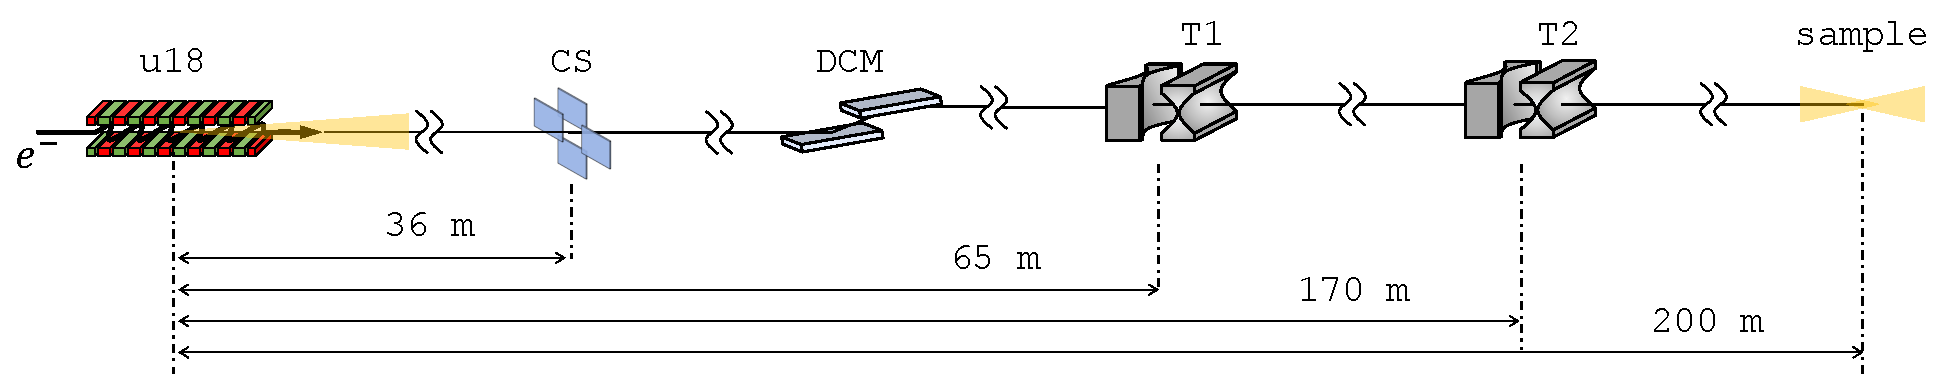
\includegraphics[width=0.99\textwidth]{figures/beamline.pdf}
    \caption{Schematic view of the beamline with the distances used in the simulations. The source is an undulator u18 set to $K$~=~1.851 (7 keV at first harmonic). CS is the ``coherence slit" that controls the coherent fraction. DCM is the double crystal monochromator (not used in the calculations). T1 and T2 are the two transfocators, idealized in single parabolic lenses. Observation plane (sample) is at 200 m from the source. 
    }
\end{figure}
\twocolumn

% \begin{table}[]
%     \label{table:id18parameters}
%     \caption{Position of the two transfocators, slit and sample (focal point) corresponding to the ID18 beamline configuration under study. }
%     \centering
%     \begin{tabular}{l|c|c}
%          element & position [m] & comment\\
%          ID (undulator) source& 0 & U18 $N_u$~=~138 $K$~=~1.851 (7 keV)\\
%          Slit & 36 &
%          variable aperture $a_h\times a_v$
%          \\
%          Transfocator 2D & 65 &
%          \\
%          Transfocator 2D & 170 & $D$~=~\SI{105}{\meter} \\
%          sample & 200 & focal plane
%     \end{tabular}
% \end{table}

We are interested in the beam properties (intensity distribution, size, flux) at the sample plane for four cases.
The first case is selected to obtain a small spot (about \SI{5}{\micro\meter}) and the second one a large spot (more than \SI{30}{\micro\meter}). For these cases the slits are selected to match a CF$_h$=CF$_v$=~90\% for a photon energy of \SI{7}{keV}. The values are shown in Fig.~\ref{table:2Dusercases}. The cases 3 and 4 follow the same logic but the slits are opened to increase intensity at expenses of reducing coherence  (CF$_h$=CF$_v$=~70\%). 


\begin{table}[]
    \label{table:2Dusercases}
    \caption{Configurations selected for 2D simulations. Slit aperture ($a_h$ or $a_v$) is selected for obtaining $CF_h=CF_v=$~90\% in cases 1 and 2, and $CF_h=CF_v=$~70\% in cases 3 and 4. 
    }
    \begin{tabular}{c|c|c|c|c|c}
         case h/v & $a_h/a_v$ [\SI{}{\micro\meter}] & $f_1$ [m] & $f_2$ [m] & $R_1$ [\SI{}{\micro\meter}]& $R_2$ [\SI{}{\micro\meter}] \\
         \hline
1 h &      40.3 & 46.1 &     26.5 &     641.9 &     369.5 
\\
1 v &      227.0 & 15.0 &     22.2 &     209.4 &     309.6 
\\
\hline
2 h &      40.3 & 25.1 &     21.3 &     349.1 &     296.3  
\\
2 v &      227.0 & 42.2 &     55.6 &     588.6 &     775.3 
\\
\hline \hline
3 h &      85.1 & 46.1 &     31.8 &     641.9 &     443.7 
\\
3 v &      506.7 & 85.2 &     27.8 &     1187.4 &     387.6  
\\
\hline
4 h &      85.1 & 25.1 &     20.7 &     349.1 &     288.7 
\\
4 v &      506.7 & 42.2 &     55.7 &     588.6 &     776.0 

    \end{tabular}
\end{table}


\section{Results of multi-optics simulations}
\label{sec:complete-beamline}

Calculations are done using different methodologies, implemented in four different software codes. 

\subsection{Source propagated up to the entrance slit}

We first calculated the illumination at the entrance slit plane. The beam at this position comes from the free propagation of the undulator emission, therefore it has the same coherence fraction as the source. The intensity distribution is shown in Fig.~\ref{fig:intensityat36m}, where the horizontal and vertical profiles calculated by Wofry1D and SRW-ME are compared. The effect of the partial coherence is important: a coherent beam would give very different values \todo{add numbers? repeat the simulations here}. \todo{may be comment 1) that the coherent illumination if different for SRW (zero emittance) than for Wofry1D (zeroth mode), and 2) we could calculate precisely the FWHM values of the profiles and compare with the typical analytical convolution calculation.}   

\todo{Look at the comparison... they have significant differences... Questions/Comments: 
\begin{itemize}
    \item  In Figs 2 and 3 I added the SRW profiles (extracted in OASYS with SRW ME output files) they are small differences... In Fig 3 I also added the DoC SRW (not in Fig. 2 as I do not have the .1 and .2 files). The Doc and 1st harmonoc are very different... to be discussed! 
    \item The division by the intensity for getting DoC adds a lot of noise when the intensity is small. Can we compare CSD((x1+x2)/2,(x1-x2)/2) instead? 
    \item I always have doubts if my factor ()/2 is correctly set.
\end{itemize}
}


\newpage
\onecolumn
\begin{figure}
    \label{fig:CSD_SRW_vs_I_source}
    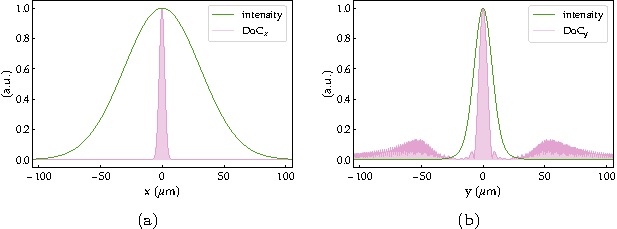
\includegraphics[width=0.75\textwidth]{CSD_SRW_vs_I_source.pdf}
    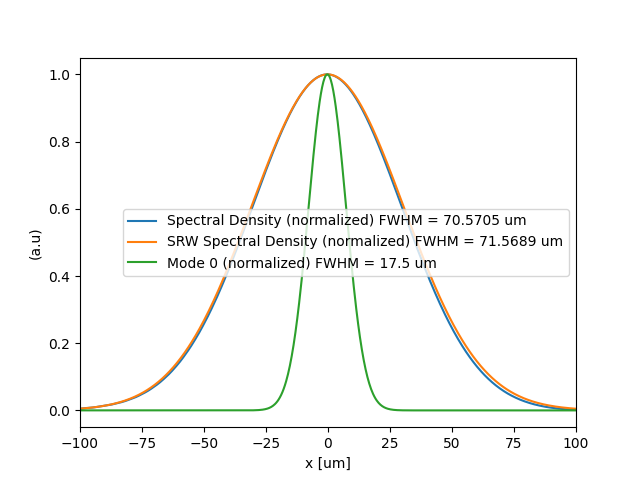
\includegraphics[width=0.35\textwidth]{figures/CSD_WOFRY1D_vs_I_source_h.png}
    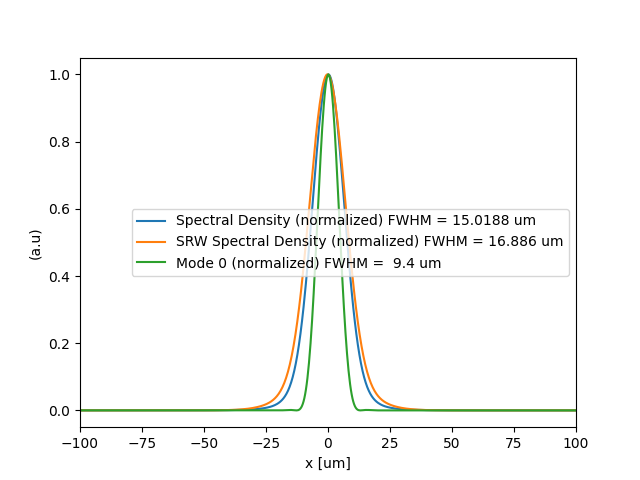
\includegraphics[width=0.35\textwidth]{figures/CSD_WOFRY1D_vs_I_source_v.png}
    \caption{Calculations @source. Top: SRW, bottom: WOFRY1D.
SRW (top): Horizontal FWHM: 73.08 [um]. 
Vertical FWHM: 18.28 [um]
Coherence length H: 6.13 [um]. 
Coherence length V: 8.53 [um].
    }
\end{figure}

\begin{figure}
    \label{fig:CSD_SRW_vs_I_36m}
    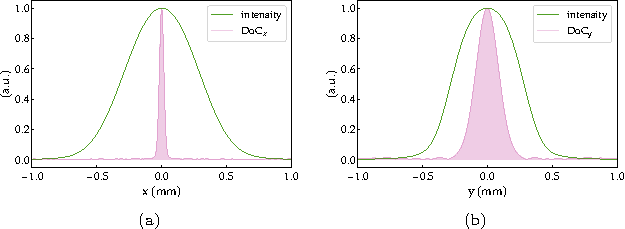
\includegraphics[width=0.75\textwidth]{CSD_SRW_vs_I_36m.pdf}
    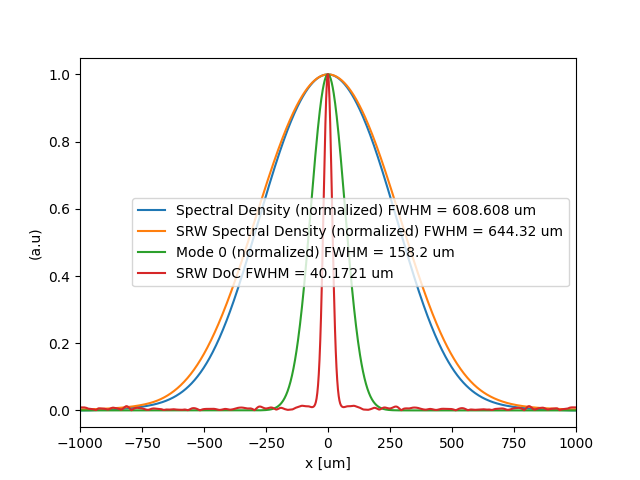
\includegraphics[width=0.35\textwidth]{figures/CSD_WOFRY1D_vs_I_36m_h.png}
    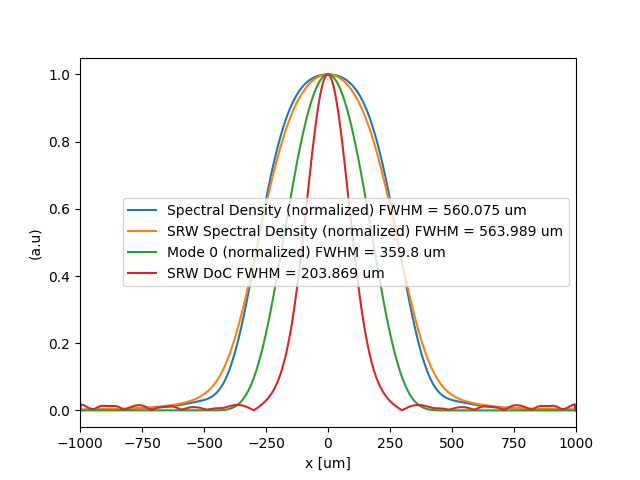
\includegraphics[width=0.35\textwidth]{figures/CSD_WOFRY1D_vs_I_36m_v.png}
    
    \caption{Calculations @36m. Top: SRW, bottom: WOFRY1D.
    
    SRW (top): 
    Horizontal FWHM: 649.53 [um].
    Vertical FWHM: 569.21 [um].   Coherence length H: 44.74 [um].
    Coherence length V: 206.90 [um].
    }
\end{figure}

\twocolumn


\newpage
\begin{figure}
    \label{fig:CSD_SRW_source}
    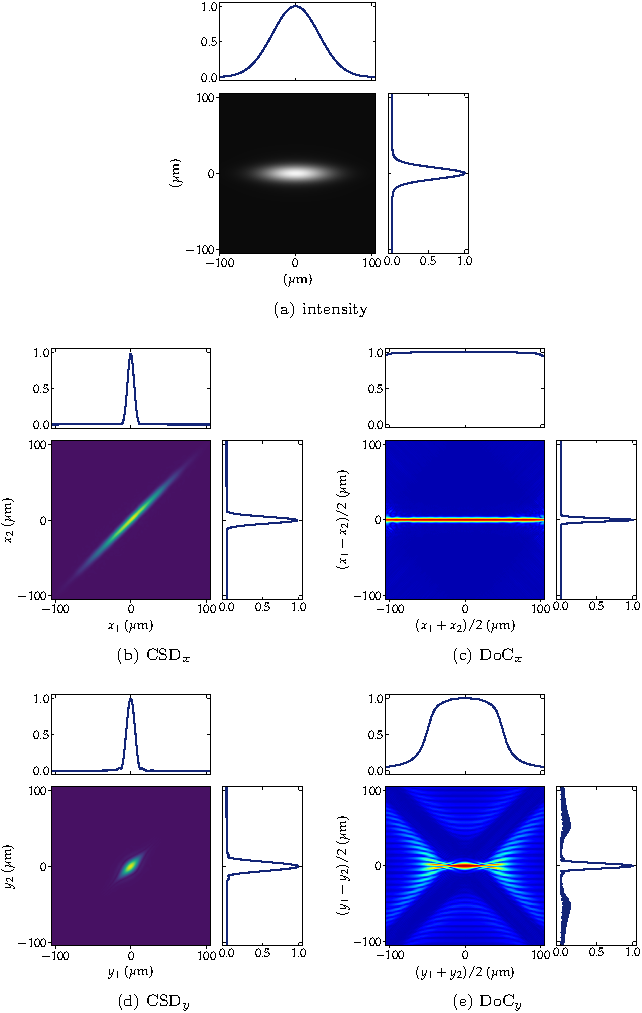
\includegraphics[width=0.99\textwidth]{SRW_CSD_source.pdf}
    \caption{SRW calculations @source}
\end{figure}

\begin{figure}
    \label{fig:CSD_SRW_source}
    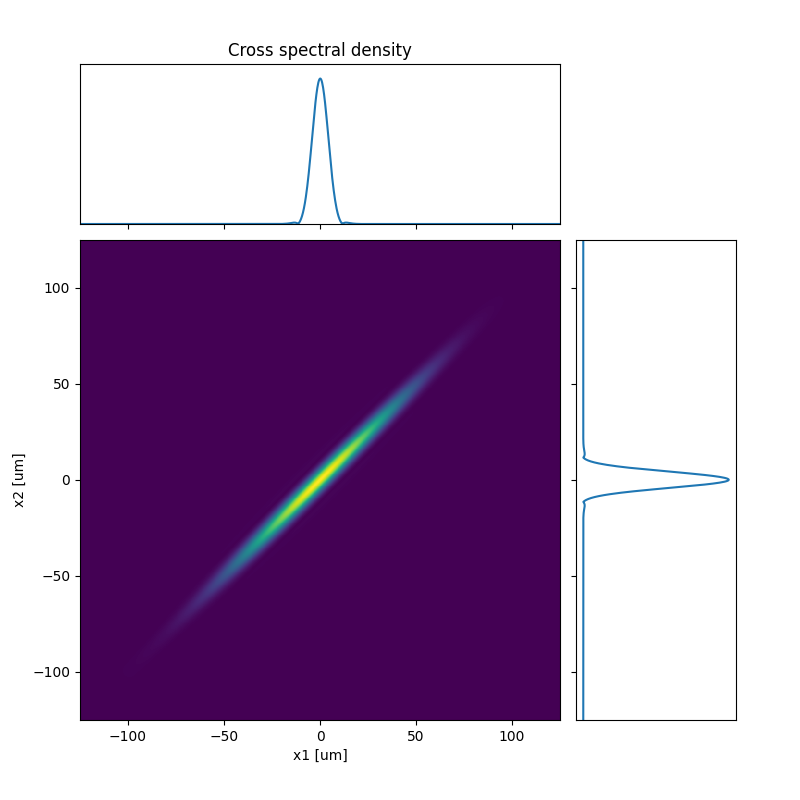
\includegraphics[width=0.49\textwidth]{figures/WOFRY1_CSD_source_h.png}
    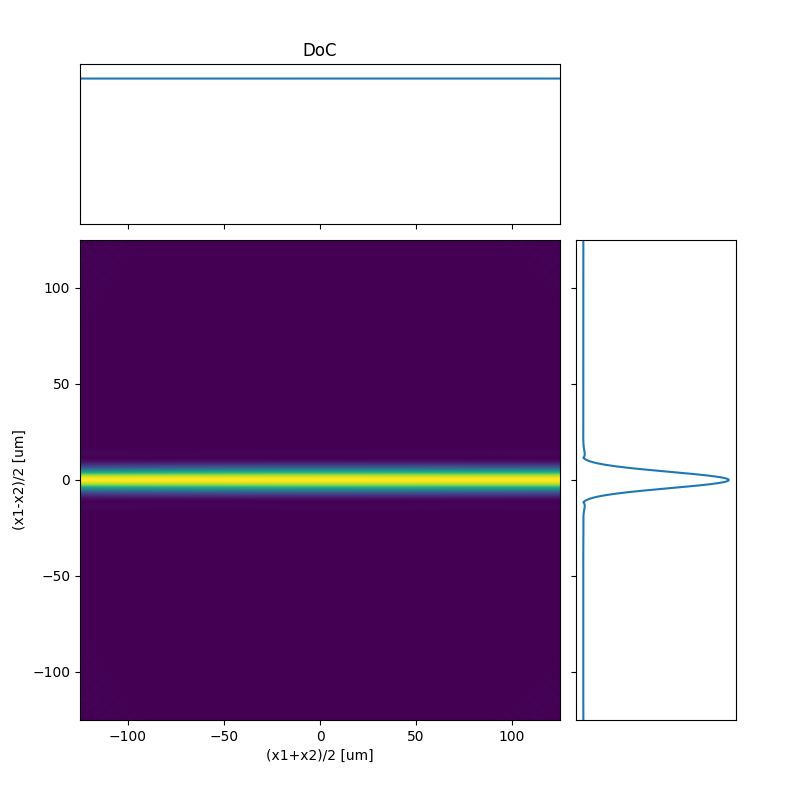
\includegraphics[width=0.49\textwidth]{figures/WOFRY1_CSD2_source_h.png}
    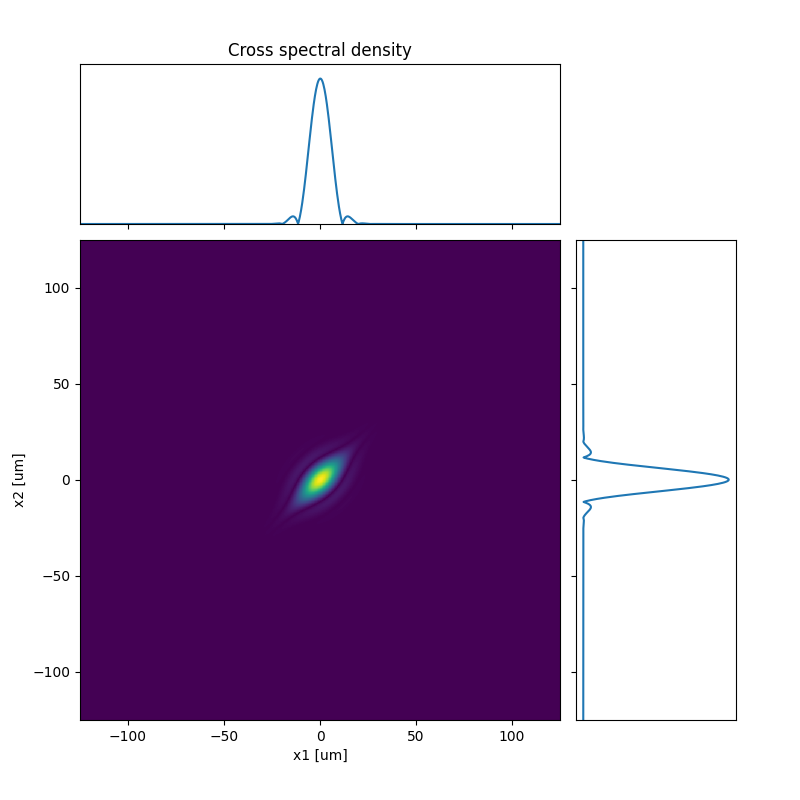
\includegraphics[width=0.49\textwidth]{figures/WOFRY1_CSD_source_v.png}
    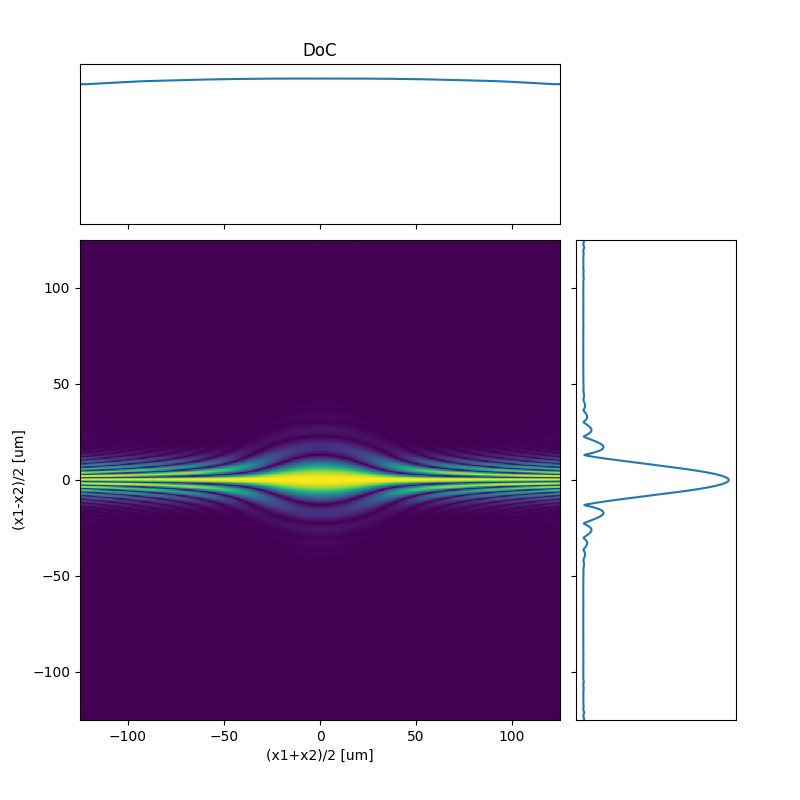
\includegraphics[width=0.49\textwidth]{figures/WOFRY1_CSD2_source_v.png}
    \caption{WOFRY1 calculations @source}
\end{figure}


\newpage

\begin{figure}
    \label{fig:CSD_SRW_36m}
    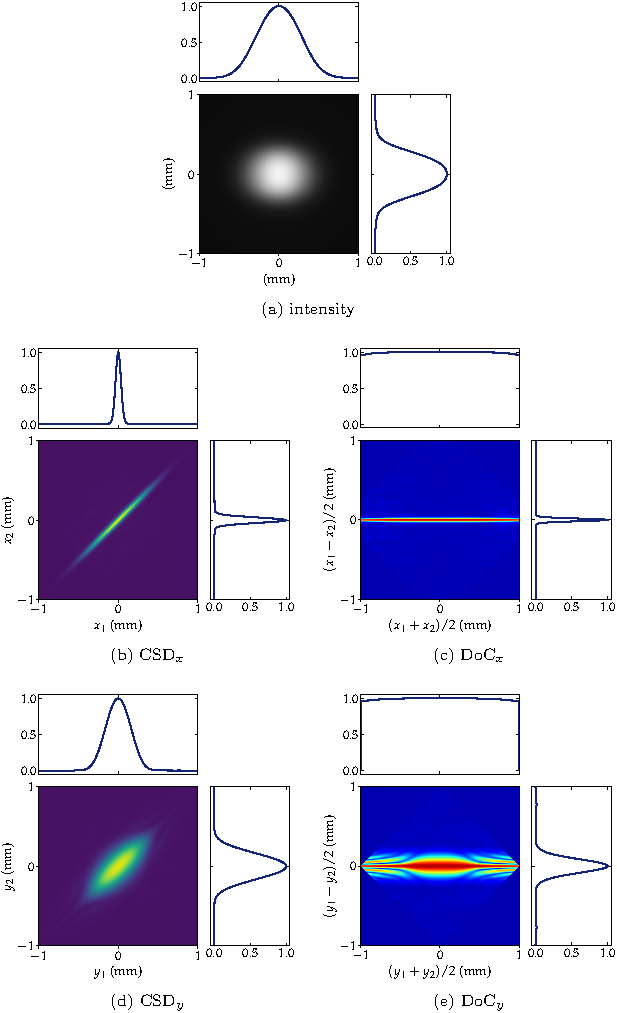
\includegraphics[width=0.99\textwidth]{SRW_CSD_36m.pdf}
    \caption{SRW calculations @36m}
\end{figure}

\begin{figure}
    \label{fig:CSD_SRW_source}
    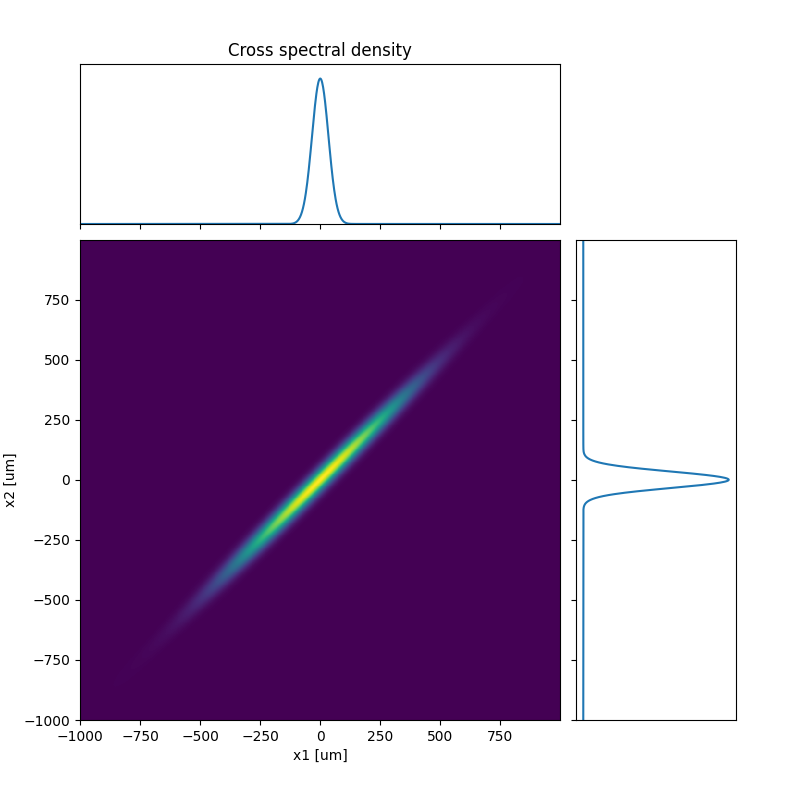
\includegraphics[width=0.49\textwidth]{figures/WOFRY1_CSD_36m_h.png}
    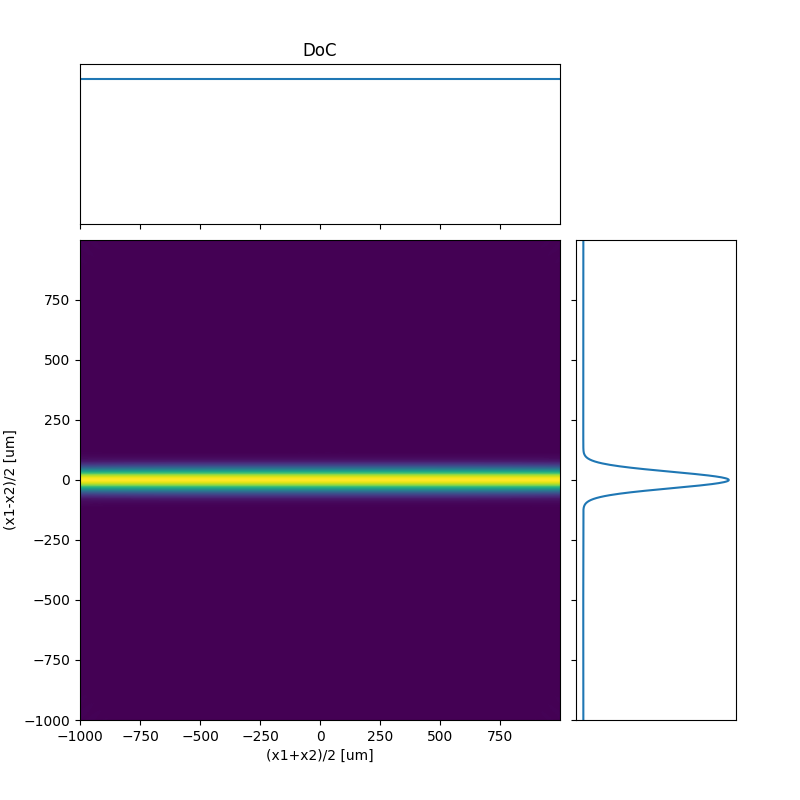
\includegraphics[width=0.49\textwidth]{figures/WOFRY1_CSD2_36m_h.png}
    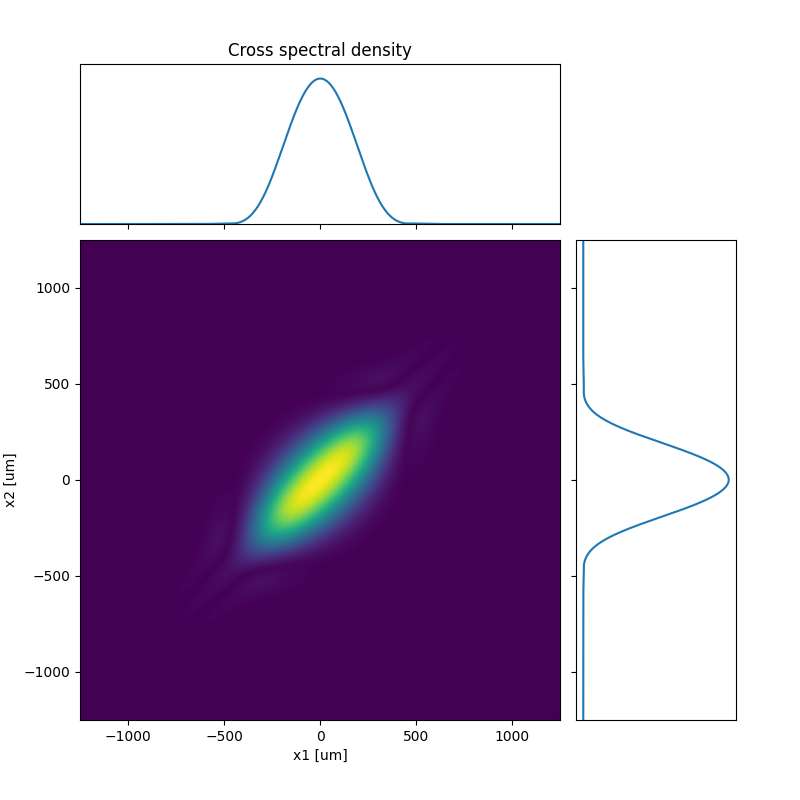
\includegraphics[width=0.49\textwidth]{figures/WOFRY1_CSD_36m_v.png}
    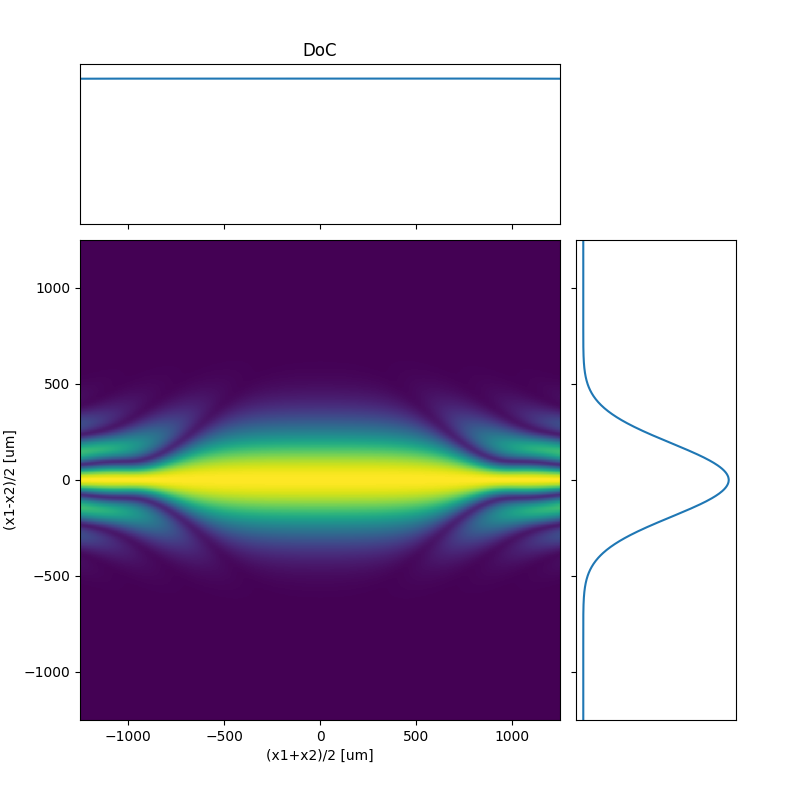
\includegraphics[width=0.49\textwidth]{figures/WOFRY1_CSD2_36m_v.png}
    \caption{WOFRY1 calculations @36m}
\end{figure}

\newpage

% \inred{Info on Figs~\ref{fig:CSD_SRW_source} and \ref{fig:CSD_SRW_vs_I_source}:}
% INFO: >>> intensity bis7.0keV intensity.dat
% INFO: Horizontal FWHM: 73.08 [um]
% INFO: Vertical FWHM: 18.28 [um]
% INFO: >>> CSDx7.0keV 15k ME intensity.dat
% INFO: Coherence length: 6.13 [um]
% INFO: >>> CSDy7.0keV 15k ME intensity.dat
% INFO: Coherence length: 8.53 [um]


% \inred{Info on Figs~\ref{fig:CSD_SRW_36m} and \ref{fig:CSD_SRW_vs_I_36m}:}
% INFO: >>> intensity bis7.0keV intensity.dat
% INFO: Horizontal FWHM: 649.53 [um]
% INFO: Vertical FWHM: 569.21 [um]
% INFO: >>> CSDx7.0keV 15k ME intensity.dat
% INFO: Coherence length: 44.74 [um]
% INFO: >>> CSDy7.0keV 15k ME intensity.dat
% INFO: Coherence length: 206.90 [um]

\subsection{Image at sample position}

The results of intensity distribution at the sample plane are display in Figs.~\ref{fig:sim_results}(a)-(d), for results using hybrid, SRW, COMSYL and WOFRY1D codes, respectively.  Beam dimensions are obtained by calculating the full width at half maximum (FWHM) from the intensity distrubution at one direction, resulting by integrating the other direction. They are displayed in the plots, and summarized in Table~\ref{table:comparison}.
The results for case 1 shows an horizontal profile mostly triangular with shoulders that evidence small diffraction fringes. The fringes are more resolved in the vertical direction. Case 2  presents in horizontal a soft Gaussian-like profile, but in vertical important symmetric shoulders are remarked. Case 3 shows a smooth Gaussian profile in horizontal and a small shoulder with fringes in vertical. Case 4 shows a conventional smooth profile in horizontal but an original three-lobe plateau in vertical. This variety of profile distribution demonstrates how relevant the diffraction effects are, which modulate the beam shape in a non-trivial way.  

\newpage
\onecolumn

\begin{figure}
    \label{fig:sim_results}
    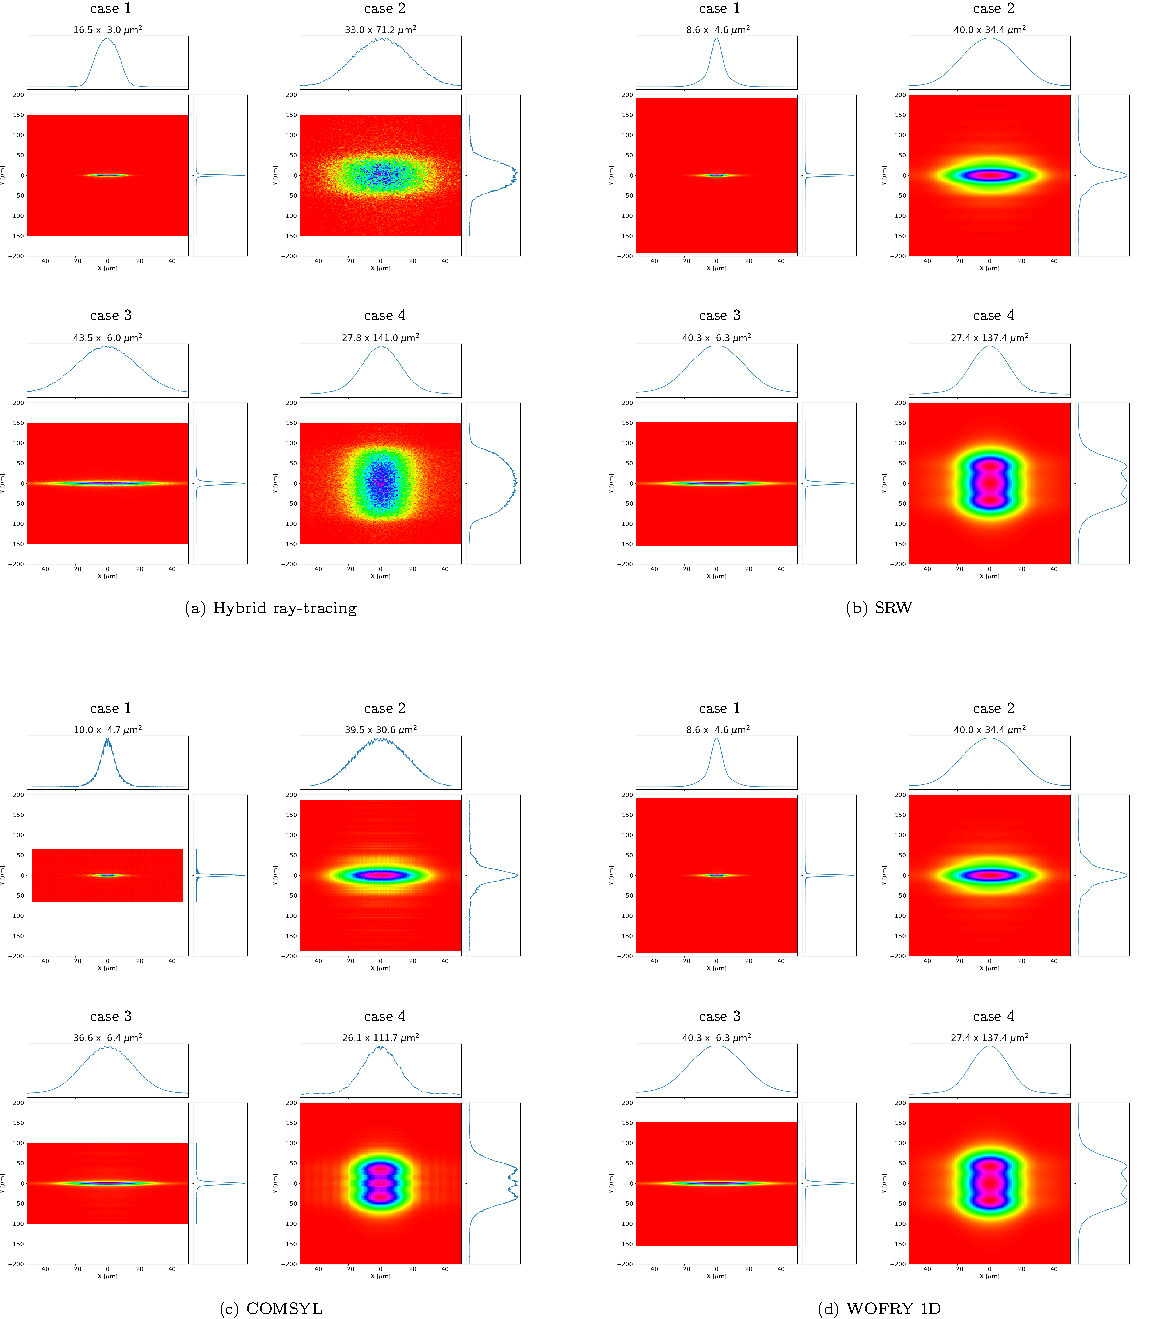
\includegraphics[width=0.85\textwidth]{figures/fig_sim_results.pdf}
    \caption{Calculations of the intensity distribution at the focal plane for the cases listed in Table~\ref{table:2Dusercases}.}
\end{figure}


% \begin{figure}
%     \label{fig:hybrid}
%     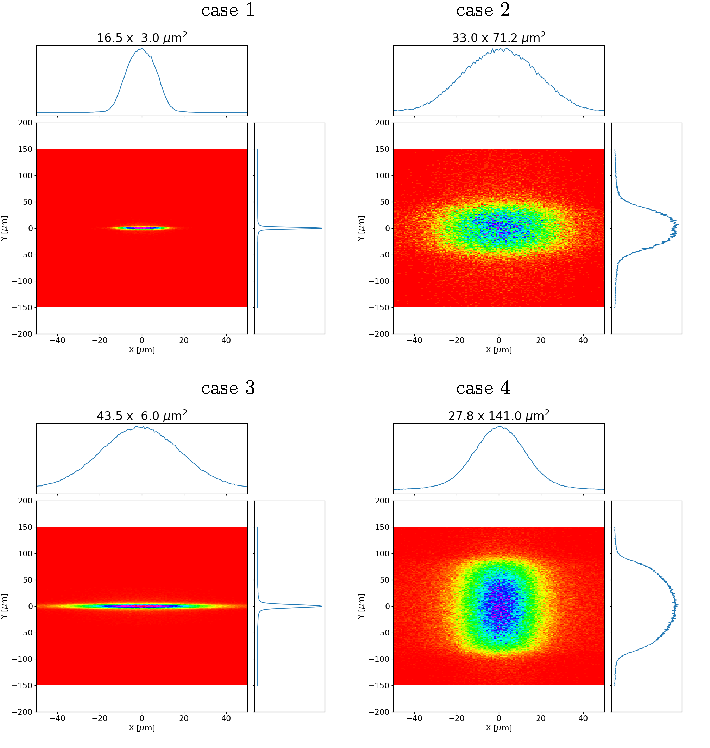
\includegraphics[width=0.99\textwidth]{figures/fig_hybrid.pdf}
%     \caption{Hybrid ray-tracing calculations of the intensity distribution at the focal plane for the cases listed in Table~\ref{table:2Dusercases}.}
% \end{figure}

% \begin{figure}\label{fig:srw}
%     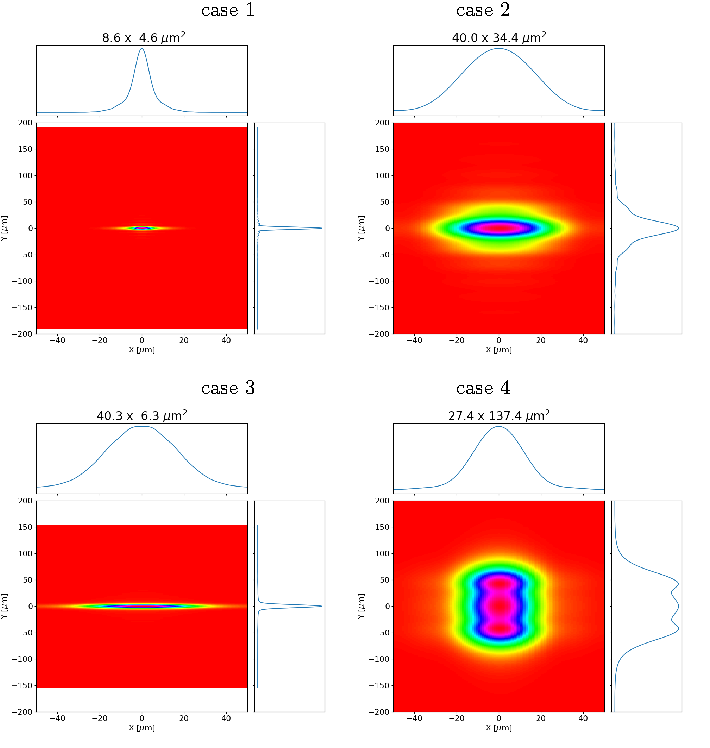
\includegraphics[width=0.99\textwidth]{figures/fig_srw.pdf}
%     \caption{Multi-electron SRW calculations of the intensity distribution at the focal plane for the cases listed in Table~\ref{table:2Dusercases}.}
% \end{figure}


% \begin{figure}\label{fig:comsyl}
%     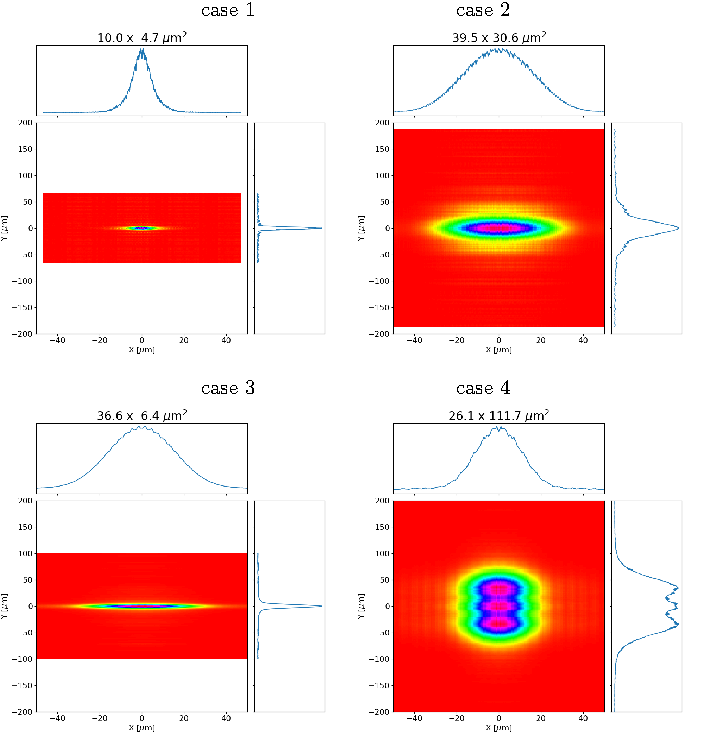
\includegraphics[width=0.99\textwidth]{figures/fig_comsyl.pdf}
%     \caption{COMSYL calculations of the intensity distribution at the focal plane for the cases listed in Table~\ref{table:2Dusercases}.
%     }
% \end{figure}


% \begin{figure}\label{fig:2DWofry1D}
%     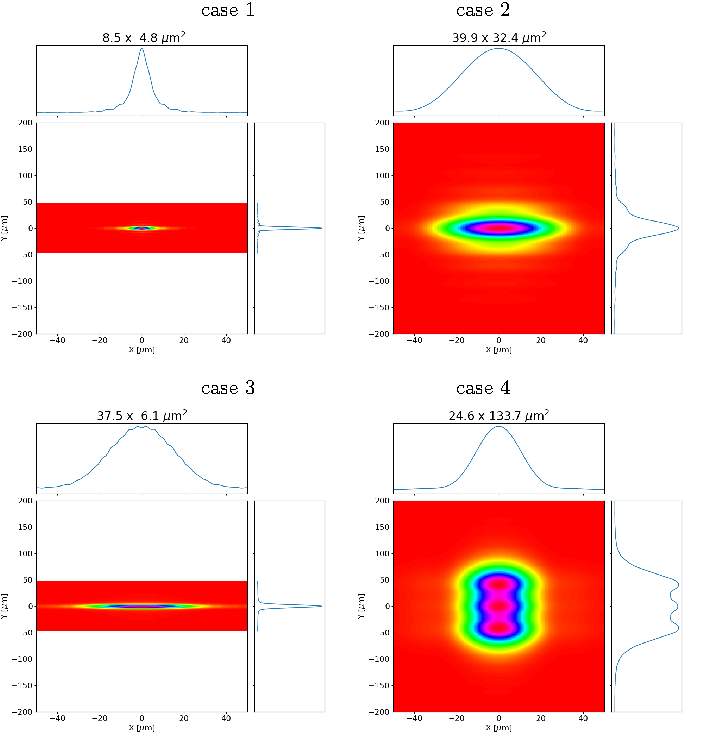
\includegraphics[width=0.99\textwidth]{figures/fig_wofry.pdf}
%     \caption{2D intensity distribution at the focal plane. It has been constructed from the Wofry1D calculations.
%     }
% \end{figure}

\newpage

\twocolumn


\begin{table}[]
    \label{table:comparison}
    \caption{Comparison of sizes (FWHM, in \SI{}{\micro\meter}) calculated with different methods for the cases defined in Table~\ref{table:2Dusercases}.
    In brackets, the values for the fully coherent beam (single electron with SRW, first coherent mode with COMSYL/WOFRY), and zero emittance with Hybrid). \todo{flip columns}
    }
    \centering
    \begin{tabular}{p{0.05\textwidth}|c|c|c|c|c}
         case h/v &
         Wofry1D&
         COMSYL&
         SRW&
         Hybrid \\
         \hline
1 h  & 8.5(8.1)    & 10.0 (9.9)  & 8.6 (7.5)   & 17.3 (17.5) \\
1 v  & 4.8(4.8)    & 4.7 (5.1)   & 4.6 (4.6)   & 3.3 (3.1) \\
\hline
2 h  & 39.9(38.2)  & 39.5 (39.5) & 40.0 (36.1)  & 39.9 (37.5) \\
2 v  & 32.4(29.6)  & 30.6 (29.3) & 34.4 (29.6)  & 74.0 (75.3) \\
\hline
3 h  & 37.5(29.0)  & 36.6 (28.1) & 40.3 (28.4)  & 43.3 (33.0) \\
3 v  & 6.1 (4.9)   & 6.4 (5.7)   & 6.3 (4.6)    & 6.5 (5.8) \\
\hline
4 h  & 24.6(19.1)  & 26.1 (18.6)  & 27.4 (18.0)   & 27.1 (18.8) \\
4 v  & 133.7(110.3)& 111.7 (90.4) & 137.4 (132.0) & 150.2 (159.8) \\
    \end{tabular}
\end{table}

Hybrid ray-tracing for the four cases defined in Table~\ref{table:2Dusercases} are shown in  Fig.~\ref{fig:sim_results}(a). One can observe that the intensity distributions as not as structured as for the wave-optics methods (e.g. the three-lobe plateau in case 4v is not reproduced). Values of FWHM are in consonance with full wave-optics calculations for most cases (with the exception of two particular cases:
1h (hybrid \SI{16.5}{\micro\meter} Wofry1D \SI{8.5}{\micro\meter}),
2v (\SI{71.2}{\micro\meter} Wofry1D \SI{32.4}{\micro\meter}). They will be discussed in the next section.


SRW-ME results for the four cases are shown in Fig.~\ref{fig:sim_results}(b). The good convergence of the values displayed is guarantee by a convergence analysis described in Appendix~\ref{appendix:srw}.
It was used to determine the minimum number of electrons that produce accurate results. The SRW-ME simulations for the cases analyzed converge with only a few thousands electrons, that can be run in less than one hour in a node with 28 CPUs totalizing 256 GB. The reason is that the beam after the slit has a relatively high CF. 


COMSYL requires high performance computing (HPC) to perform full CMD of undulator beam, by
solving the Friedholm problem and obtain the full 2D eigenfunctions (coherent modes) and eigenvalues.
Simulation of the source with COMSYL took 55 min using 28 x 3.30 GHz CPUs of 251.82 GB RAM, for getting 174 modes of 1691 $\times$ 563 pixels.
The modes calculated by COMSYL are loaded in the OASYS environment \cite{codeOASYS} to propagate the modes along the beamline.
The propagation uses 2D zoom propagator and the optical elements available in WOFRY. Results are shown in Fig.~\ref{fig:sim_results}(c). 
The beam profiles calculated with COMSYL are a bit noisy, which could be improved by increasing the source sampling and further optimizing the propagation parameters. 


WOFRY 1D results are shown in Fig.~\ref{fig:sim_results}(d). The 1D intensity profile for one direction is obtained from the summation of several modes. High modes have very low eigenvalue and it is enough to consider only 10 modes for reproducing more that 99\% of the spectral density. The 2D intensity distribution shown in Fig.~\ref{fig:sim_results}(d) is obtained combining the calculated horizontal and vertical 1D profiles via the outer product. We can observe in the intensity distributions the same structures due to the diffraction effects than were observed with the other calculation methods. 
The agreement between the results of Wofry1D in Fig.~\ref{fig:sim_results}(d) with SRW - Fig.~\ref{fig:sim_results}(b) - is striking. All intensity distributions reproduce exactly the same features, and the FWHM values are different in less than 12\%, a value that is compatible with the errors of the simulations (discussed in section~\ref{sec:discussion}). This results validates the 1D CMD method proposed here, whose requirements in computer power are extremely low (it runs very fast in an averaged laptop).  

The specific numeric value for sizes calculated with the different methods (Table~\ref{table:comparison}) depends not only on the code itself, but also on the particular specific parameters in each method (number of pixels for sampling wavefronts, propagation parameters, etc.). To estimate the calculation error in the final size numbers, we vary randomly these specific parameters in a reasonable range (e.g., 10\%). The evaluation of the mean size and the dispersion (standard deviation) of the sizes obtained give an good estimation of the error in this parameter. This exercise would take a considerable computational effort using 2D methods, but it can be easily done with Wofry1D. We run 200 cases with 10\% random variation in the values in number of pixels and magnification factor in drift spaces. The obtained sizes (horizontal $\times$ vertical) are  
8.49 $\pm$ 0.60 $\times$ 4.97 $\pm$ 0.37 \SI{}{\micro\meter}$^2$ (case 1),
39.94 $\pm$ 2.98 $\times$ 32.77 $\pm$ 2.69 \SI{}{\micro\meter}$^2$ (case 2),
36.39 $\pm$ 2.89 $\times$ 6.12 $\pm$ 0.51 \SI{}{\micro\meter}$^2$ (case 3), and
24.18 $\pm$ 1.80 $\times$ 133.44 $\pm$ 10.06 \SI{}{\micro\meter}$^2$ (case 4). We confirmed that the values given in Fig.~\ref{fig:sim_results}(d) are within these error intervals.


The calculated beam sizes should be completed with flux. At \SI{7}{keV}, the undulator in the configuration selected emits a flux of 1.5 10$^{15}$ photons/s/0.1\%bw. Each of the three elements studied (slit, lens -1 and lens-2) absorb part of the flux. The estimation of the absorption by the slit can be done using simple geometrical arguments, and the absorption by the slits depend on the average Be thickness presented to the beam. The linear attenuation coefficient of Be at 7 keV is $\mu=$~\SI{3}{\centi\meter}$^{-1}$, giving 1.45\% attenuation for a \SI{50}{\micro\meter} thick layer (like lens thickness used in simulations\footnote{In the simulations the horizontal and vertical focusing are separated in two lenses, with accumulated thickness \SI{100}{\micro\meter} thus absorption 3\%}). For the case 1 simulations we extracted the absorption for the different absorbing elements (slit, lens-1 and lens-2) in the case of partial coherence and also for full coherence (see Table~\ref{table:absorption}).
There is excellent agreement for partial coherence. For full coherence, the Wofry1D results are different than the SRW+Hybrid, because the geometry of the 1st coherent mode used to represent the full coherent beam is not the same as the geometry of the filament beam (used in SRW and Hybrid). We note a high absorption in lens-2, due to the fact that in this case the lens-2 is overilluminated, therefore the \SI{1}{\milli\meter} physical aperture absorbs considerably the beam.

\begin{table}[]
    \label{table:absorption}
    \caption{Comparison of beam intensity attenuation in percent by the slit, lens-1 and lens-2 for the partial coherent beam, 
    % coherent beam (first coherent mode in Wofry1D, filament beam in SRW, zero emittance in Hybrid) and for the partial coherent beam,
    for the four cases studied.
    The Wofry1D data shown here comes after combining the horizontal and vertical wavefronts using the outer product. 
    }
    \centering
\begin{tabular}{l|lll|lll|lll}
case & \multicolumn{3}{c|}{slit} & \multicolumn{3}{c|}{lens-1} & \multicolumn{3}{c|}{lens-2} \\
\hline
     & \rot{Wofry1D} & \rot{SRW} & \rot{Hybrid}
     & \rot{Wofry1D} & \rot{SRW} & \rot{Hybrid}
     & \rot{Wofry1D} & \rot{SRW} & \rot{Hybrid}
\\
\hline
%    &          &      &        &          &      &         &          &       &         \\
%1      &   87.0   & 96.6 & 96.7   & 7.6      & 7.4  & 5.2     & 48.3     & 51.3  & 53.0   \\
1       &   97.6   & 97.6 & 97.2   & 7.9      & 7.6  & 5.2     & 50.7     & 51.1  & 52.6   \\
% 2c    &   87.0   & 96.6 & 96.7   & 6.7      & 6.4  & 4.3     & 3.8      & 3.7   & 3.3    \\
2       &   97.6   & 97.6 & 97.2   & 7.0      & 6.6  & 4.3     & 3.9      & 3.7   & 3.3    \\
% 3c    &   55.9   & 86.0 & 85.6   & 5.4      & 6.11 & 4.7     & 17.1     & 22.7  & 26.6   \\
3       &   89.5   & 90.2 & 88.6   & 6.3      & 6.1  & 4.6     & 23.4     & 21.8  & 25.2   \\
% 4c    &   55.9   & 86.0 & 85.6   & 6.8      & 7.73 & 6.4     & 3.6      & 3.6   & 3.6    \\
4       &   89.5   & 90.2 & 88.6   & 8.0      & 7.7  & 6.2     & 3.8      & 3.6  & 3.6   \\
\end{tabular}
\end{table}

% -----------------------------------------------------------------
% -----------------------------------------------------------------
\section{Discussion}
\label{sec:discussion}
% -----------------------------------------------------------------
% -----------------------------------------------------------------

% Our discussion follows a hierarchical approach, as discussed in \citeasnoun{hierarchical}, with the idea of balancing accuracy and computational effort, to subsequently select and use the most advantageous method for the analyzed problem. 
% This multi-method analysis will also help to validate the new 1D CMD method introduced in this work. The results of the Wofry1D results are compared with other well-known simulation packages. 


There is good agreement in focal size FWHM values in all methods (see Table~\ref{table:comparison}), but also in the shape of intensity distributions, in particular for the wave optics methods - compare Figs.~\ref{fig:sim_results}(b)-(d). 

Regarding computer resources, the Wofry1D code can be run in a few seconds in a laptop, whereas the simulation of the full CMD with COMSYL required about 1h (for 1691 x 563 pixels, 174 modes) using 1 node of 28 cores. This source is then reused for propagating the different configurations. Each configuration required a full SRW-ME with 5000 electrons run in also about 1h in a similar configuration. 

\todo{a possible paragraph discussing surface errors. Just to show it as a proof of concept: FEM at the white mirror, slope error at the mirros, FEM at the monochromator... Cons: it will be done with only Wofry1D (too much work for the full collection of codes); the results will not change what we have}


\todo{A possible discussion of the Gaussian Shell-model. I am not much in favor of including the GSM here, but it can be done. Main points for the discussion:

\begin{itemize}
\item Discuss how to match the GSM with undulator parameters: there are several possibilities... I prefer matching the size and CF. 
\item Compare Hermite-Gaussian modes with numerical modes. There are similar nut not identical. For incoherent sources the GSM may be a good approximation, for pretty coherent sources not. 
\item Show that propagation of GSM modes is very different than propagating undulator modes. Indeed, because $\sigma \sigma' = \lambda / (4 \pi)$ in GSM and with $2\pi$ in undulator either the size at the source or the propagated size is wrong with GSM.
\item Analytical propagation of the modes (as described by Vartanyants et al.) only works for ideal elements, and Gaussian slits. They fail in simulating structures like those that we obtain, because they are originated by the slit, which is non-Gaussian.
\end{itemize}
}


% \subsection{Hybrid ray-tracing}

% The simulation results for the four cases studied using the hybrid method indicate that, although this method does not reproduce exactly the intensity distibution given by full partial coherent optics, the numerical values are approaching the good ones, but with two exceptions: the case 
% 1h (hybrid \SI{16.5}{\micro\meter} Wofry1D \SI{8.5}{\micro\meter}) and the case 
% 2v (\SI{71.2}{\micro\meter} Wofry1D \SI{32.4}{\micro\meter}). 
% We remark that these thee cases have in common that the $f_1$ value in use is close to $f_1$~=~\SI{40}{\meter} that corresponds to the singularity in the analytical (geometrical optics) calculations, when the lens-1 focuses on lens-2. A detailed study with hybrid was performed to calculate the FWHM for all possible values of $f_1$ (as done in Fig.~\ref{fig:focalSizes}. The result (Fig.~\ref{fig:focalSizes_hybrid}) confirms that there is good agreement everywhere except in the region close to $f_1$~=~\SI{40}{\micro\meter}.
% We thus conclude that the hybrid ray-tracing is a valid method to obtain good values of focal sizes in most cases, excepts for the case that lens-1 focus is close to the position of lens-2 ($f_1 \approx $~\SI{40}{\meter}).


% \begin{figure}
%     \centering

%     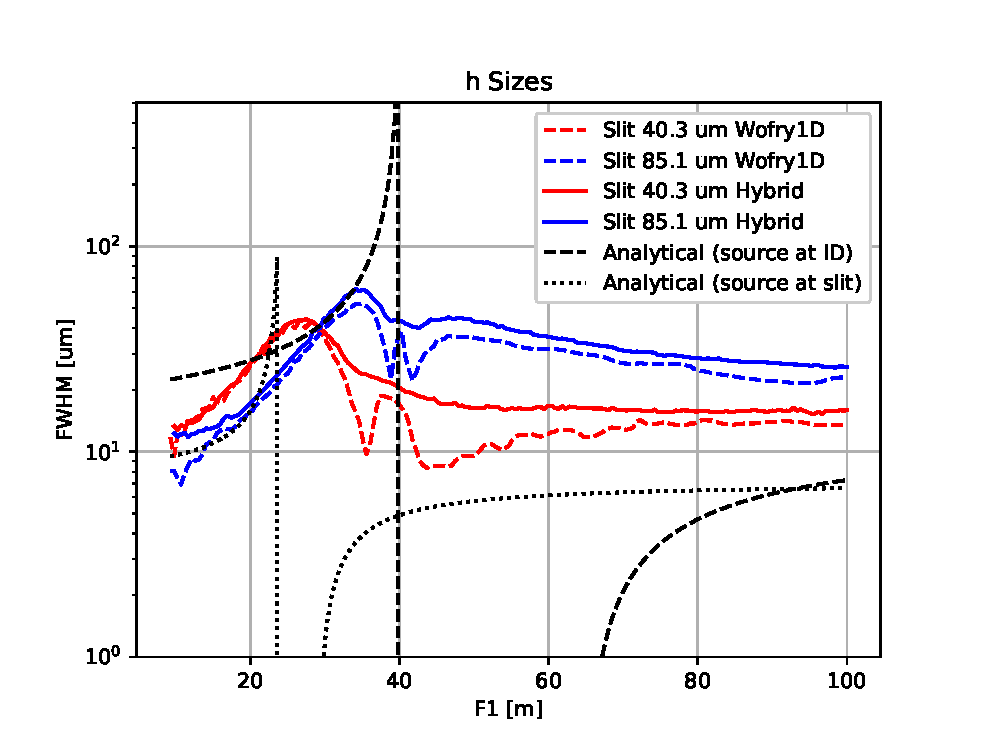
\includegraphics[width=0.95\textwidth]{figures/sizes_h_hybrid.eps}
%     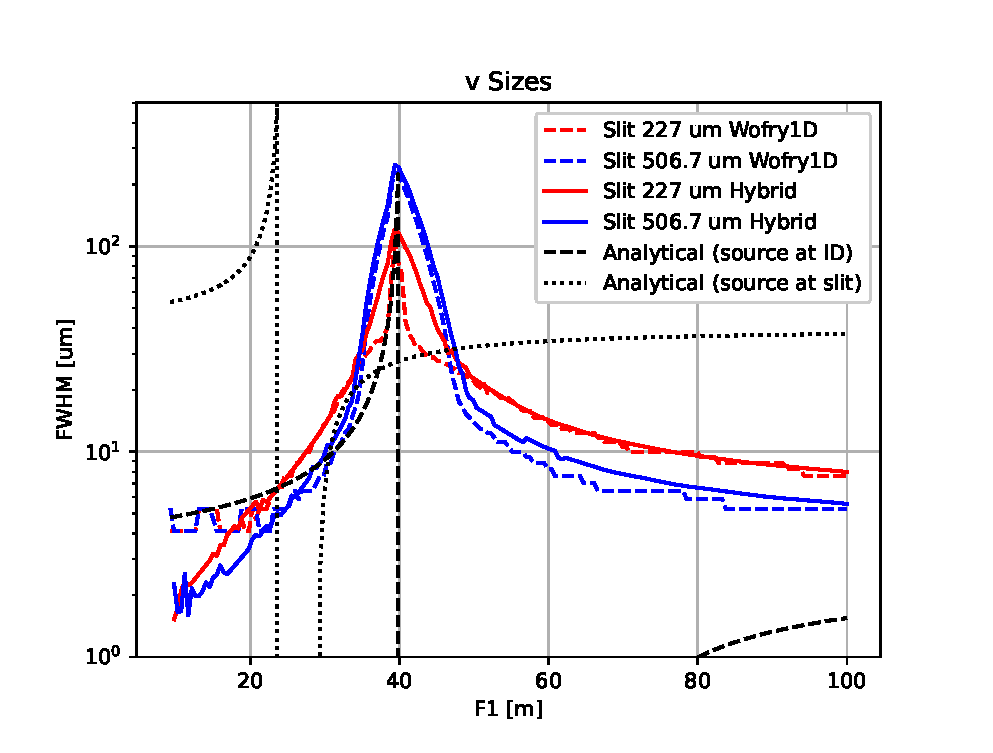
\includegraphics[width=0.95\textwidth]{figures/sizes_v_hybrid.eps}
        
%     \caption{Focal sizes obtained by hybrid ray-tracing method, for two slit aperture cases, compared with values from Wofry1D  (from Fig.~\ref{fig:focalSizes}).}
%     \label{fig:focalSizes_hybrid}
% \end{figure}

% \subsection{Further simulations}

The simulations presented, motivated by the ID18 project, use a simplified optical layout. A more complete study including the other optical elements, other transfocator configurations will be presented elsewhere, also for different energies and implementing the effect of surface errors due to thermal load and surface finish. 

% We have also calculated the beam evolution in the neighbourhood of the sample position for the four cases studied (see Fig.~\ref{fig:caustic}). From these plots one can obtain the position of the best focus and the depth of focus. The depth of focus (measured as the distance where the peak value is reduced by 15\%) is larger than two meters (except for the cases 1v, 3v). \todo{redo these plots and compare with SRW... otherwise supress?}

% In some cases there is a mismatch between the position of the best focus and its expected position (the sample position, at the zero abscissas). This effect, certainly due to an error in setting $f_2$, may have several origins. 

% For pairing two transfocators, the algorithm chosen to calculate the $f_2$ value consist in analyzing the wavefront at the lens-2 position, find a corrector refractive object that would transform the incoming wavefront in a converging wavefront (see section \ref{sec:refractorCorrector}), and fit the radius at the center. We then get the $R_2$ and therefore the $f_2$ value. In addition, to obtain smooth $(f_1,f_2)$ curves in Fig.~\ref{fig:f1f2map} we have used a Gaussian slit (see section \ref{sec:gaussianslit}). It smears out the diffraction fringes, because in an ideallized system where a point source is focused at the sample position, the recorded intensity would correspond to the diffraction pattern of the slit, that can be considered as an "object" placed in the beam (see e.g. \cite{paganin_book}). The use of a Gaussian object implies that its diffraction pattern is a Gaussian with no diffraction fringes. 

% For cases 1h, 1v, 3v (see  Fig.~\ref{fig:caustic}), there is a good agreement between the focal position obtained from the maximum of intensity on-axis (plotted at the top of the image) and our expected position (the zero in the plots). In some other cases (2v, 3h, 4h) the agreement is acceptable, taking into account that the observed depth of focus is of the order of meters. A small correction in $f_2$ would bring the best focus to its ideal position. This correction is necessary because we used a Gaussian slit for calculating $f_2$, thus neglecting some oscillations around the $(f_1,f_2)$ curves. There are two pathological cases where the algorithm used to calculate $f_2$ did not succeed: the cases 2h and 4v.
% The error in $f_2$  for case 2h is also due to the oscillations in the $(f_1,f_2)$ and can be corrected, as shown in Fig.~\ref{fig:causticcorrection}a. However, case 4v cannot be corrected because we would need a divergent lens to bring the focus of $f_1$ to the sample position. Setting $R_2=f_2=\infty$ would reduce the beam size at the sample position (Fig.~\ref{fig:causticcorrection}b), but cannot get the best focus there. However, an ad-hoc defined refractive corrector in the place of lens-2 would do the job (Fig.~\ref{fig:causticcorrection}d).  

 



%%%%%%%%%%%%%%%%%%%%%%%%%%%%%%%%%%%%%%%%%%%

% \begin{figure}\label{fig:caustic}
% \centering

% 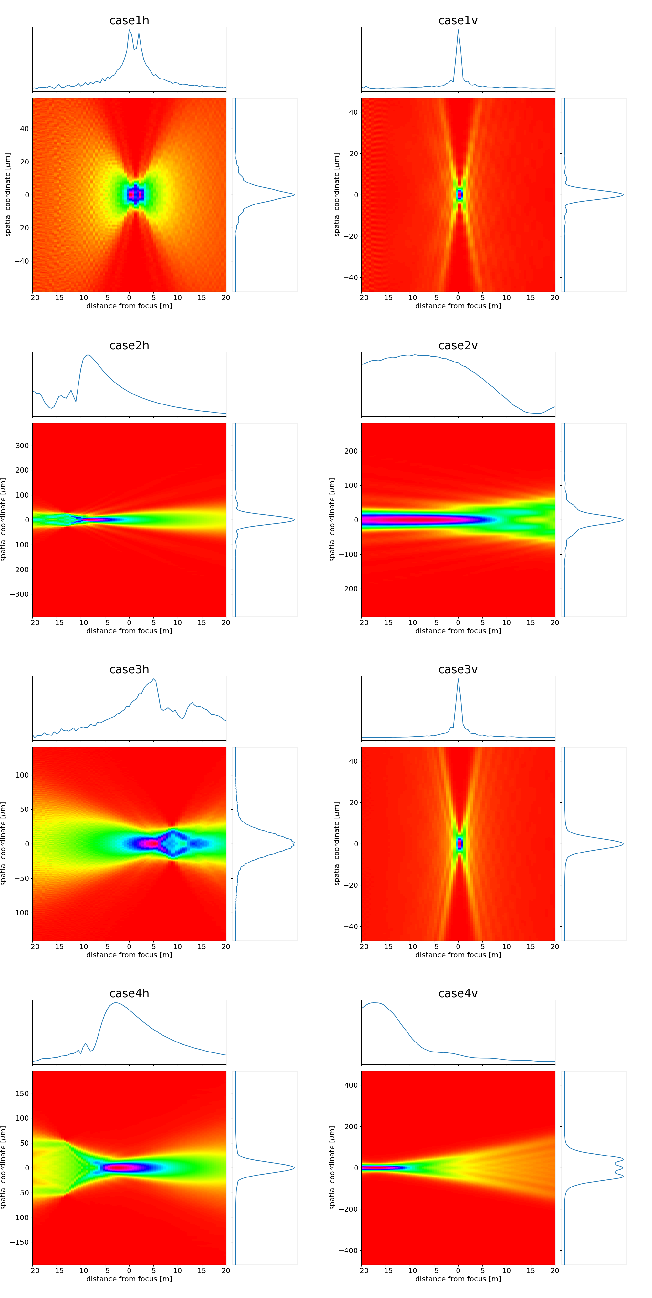
\includegraphics[width=0.99\textwidth]{figures/fig_caustic.pdf}

% \caption{Evolution of the beam size in the around the sample position for the cases listed in Table~\ref{table:2Dusercases}. The top and side graphs correspond to the profiles passing by (0,0).
% }
% \end{figure}



% \begin{figure}\label{fig:causticcorrection}
% \centering
% 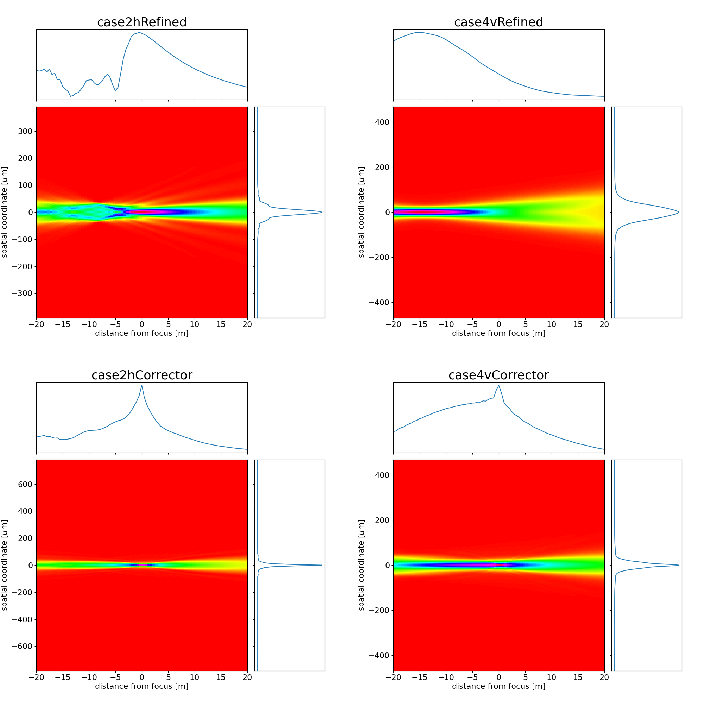
\includegraphics[width=0.99\textwidth]{figures/fig_caustic_correction.pdf}

% \caption{Evolution of the beam size in the around the sample position for the ``pathological" case 2h and 4v shown in Fig.~\ref{fig:caustic}. Top row: using corrected lens-2 with $R_2$=\SI{410}{\micro\meter} ($f_2=$\SI{29.4}{\meter}) for case 2h and $R_2=f_2=\infty$ for case 4v. Bottom: using a free-form refractive corrector instead of lens-2.
% }
% \end{figure}


% \subsection{Errors in optical surfaces}

% % \todo{Rafael, please re-read}
% The performance of X-ray optics in the new generation synchrotron beamlines is limited by the quality of the optical surfaces \cite{lengeler1999,Yabashi}. Finish errors can be divided in three families: i) height errors, associated with surface finishing (high spatial frequency), ii) figure errors, associated with deviations from ideal profile (e.g. bending, gravity sag, thermal deformations), and iii) slope errors or waviness, associated to medium spatial frequencies \cite{srio1992, signorato1997}. Finish errors in x-ray lenses can be measured by different techniques (eg. grating interferometry, x-ray speckle tracking or ptychography) and readily included in the simulations \cite{Celestre:mo5214}. Some profiles measured at ESRF using x-ray speckle tracking \cite{berujon2020} with height error RMS of the order of \SI{1}{\micro\meter} are used to verify that the focal spot produced by lenses with realistic errors is not degraded with respect to the ideal lens surface. 

% Usually the optics of new generation synchrotron beamlines is limited by the quality of the optical surface. Typically are due to surface finish (slope errors and height errors) and shape errors, often due to heat load. 
% \todo{Rafael, would you please work next paragraph. I checked that your error file (profile 1 in DABAM2D) does not produce relevant changes, thus the idea is to "mention" the errors without presenting a full study.} Surface errors in lens surfaces can be experimentally measured by different techniques (e.g. speckle tracking, ptychography) and included in the simulations. Some profiles measured at ESRF \cite{???} with height error RMS of the order of \SI{1}{\micro\meter}  are used to verify that the focal spot produced by lenses with realistic errors is not degraded with respect to the ideal lens surface. 

% The effect of finish errors in the white double-mirror system is also analyzed using a measured mirror meridional profile of \SI{2.5}{\nano\meter} height error RMS and \SI{140}{\nano\radian} RMS slope error. 

% % \todo{Philipp, please re-read}
% The heat load affect several elements of the beamline. For the beamline under consideration, the affected elements (white beam mirrors, and double-crystal monochromators) are not presented in our simulations. Finite element analysis of mirrors and crystals done for other EBS beamlines \cite{Brumund} show that the deformation height profile can be decomposed it two parts: an average bending that is possible to correct by a small readjustment of the focal length of the optical elements downstream the heated element, and a ``residual error" which remain after removing the averaged bending radius, and could only be corrected using adaptive optics. Wofry1D simulations using FEA-generated deformations at the first crystal of a monochromator placed just after the coherent slit showed no significant degradation of the focal spot, both in size and shape. This is mainly due to the low power transmitted by the coherent slit. We checked that the focused beam is almost unchanged when using a profile from FEA analysis with curvature of about \SI{1}{\kilo\meter} and residual slope errors of \SI{30}{\nano\radian}. 



% The deformation profile calculated by FEA \todo{I USED FILE: SRC\_Si\_3.0mrad\_08000eV\_mo\_Si111\_Size1\_nodalOut.out} is is loaded in a ``mirror-like" element in Wofry, as described \cite{srioLBL}. For case 1, a small degradation in the horizontal direction is found (passing from \SI{8.09}{\micro\meter} to \SI{10.21}{\micro\meter} for the first coherent mode). It is accompanied by a loss of symmetry. A large deformation in the vertical spot is observed, but a spot close to the ideal is found when a best circle is subtracted from the profile. It is then possible to correct this added curvature. Indeed, by adjusting $f_2$ \todo{I will calculate this} it is possible to compensate the effects introduced by the crystal bending due to heat load.


% finding focus https://www.optikos.com/finding-focus/

% \subsection{Practical considerations} Simulations like those presented here could be very beneficial for beamline operation, for its optimization and quick setting.  Complicated  relationships exist between the beam parameters requested by users (beam size and coherent fraction) and the beamline configuration (undulator, slit and transfocator setting). Quick simulations as done by Wofry1D could be a helpful instrument for the beamline staff to get the desired configurations. The plots shown here (e.g., $CF$ vs slit size in Fig.~\ref{fig:cf_vs_aperture}, trajectories in Fig.~\ref{fig:f1f2map}, or final size in Fig.~\ref{fig:focalSizes} could be simulated on-line and compared with results presented as look-up tables with similar aspect. We are also considering the design of a digital twin that mimics the real transfocator systems to assist beamline setting. For that, the fast simulation using the CMD method developed in Wofry1D will be an integrated component.  

% Some practical consequences can be directly deduced from the results shown here. For example, looking at Fig.~\ref{fig:focalSizes} one can observe that the same focal size can be obtained with different configurations. To get a similar size, it is better to prefer a large $f_1$ to avoid over-illuminating the lens-2 and increase transmission of lens-1. The transfocator design is simplified if we restrict the horizontal focal distance t to be smaller than the vertical $f_h>f_v$. Here, $f_v$ can be obtained with lenses focusing in 2D and $f_h$ by adding 1D lenses focusing in the horizontal plane. 

% % https://www.optikos.com/finding-focus/
% In this work we configured the transfocator to have the resulting focal position on the sample plane, an "in-focus" setup. It could also be possible to work off-focus to vary the beam size at the sample plane. The in-focus setup will generally produce the sharpest image of very small details in the image. Moreover, it will reduce the artifacts produced by the surface finish errors. Also, a larger depth of focus is obtained at this position (see e.g. Fig.~\ref{fig:causticcorrection}).

% -----------------------------------------------------------------
% -----------------------------------------------------------------
\section{Summary and conclusions}
\label{sec:summary}
% -----------------------------------------------------------------
% -----------------------------------------------------------------
We have studied a particular case of focusing a partial coherent beam (as produced by the low emittance storage ring EBS-ESRF) by a system of two transfocators (or lenses). We have verified that four simulation codes typically used to simulate synchrotron beamlines agree in the results of beam size and flux. The hybrid ray-tracing method (ShadowOUI) fails to determine fine structures in the beam intensity profiles. The three codes using physical optics (SRW-ME, COMSYL and WOFRY1D) produce essentiually the same results. Partial coherence calculations using 2D wavefronts are expensive from the computation point of view, either because many thousands of wavefronts are propagated (in SRW-ME) or because the need of diagonalizing an extremely large 4D cross-spectral function. The newly developed coherent mode decomposition of 2D CSFs (i.e. separating 1D modes for the horizontal and vertical direction) is very rapid and can be run interactively in a laptop. Its results for the particular cases simulated here agree very well with full 2D propagation methods. 
This method is available in the Wofry add-on of the OASYS suite \cite{codeOASYS}. OASYS workspaces for the simulations performed in this paper are available\footnote{{ https://github.com/oasys-esrf-kit/paper-multioptics-resources}}.

% Four cases are calculated and compared using the other methods available in OASYS, like the full 2D coherent mode decomposition using COMSYL \cite{codeCOMSYL}, the OASYS interface for the SRW \cite{codeSRW} code, and hybrid ray-tracing \cite{codeHYBRID}.


%%%%%%%%%%%%%%%%%%%%%%%%%%%%%%%%%%%%%%%%%%%%%%%%
%%%%%%%%%%%%%%%%%%%%%%%%%%%%%%%%%%%%%%%%%%%%%%%%
%%%%%%%%%%%%%%%%%%%%%%%%%%%%%%%%%%%%%%%%%%%%%%%%
\appendix

% -----------------------------------------------------------------
% -----------------------------------------------------------------
\section{The SRW propagators}
\label{sec:appendixSRWpropagators}
% -----------------------------------------------------------------
% -----------------------------------------------------------------

 The SRW propagators are grouped into three main methods for 2D wavefront propagation \cite{SRWgit}. The first main method lies under the ``standard Fresnel propagator'', which can be implemented as: (a) direct numerical calculation of the convolution integral in Eq.~\ref{eq:Fresnel} by means of nested Riemann summations; or (b) through the application of the convolution theorem:
 \begin{equation}\label{eq:FresnelConv}
\begin{split}
    E_\omega(\textbf{r}')&=\frac{k\exp{(ikL)}}{2\pi i L} E_\omega(\textbf{r}) * \exp{\bigg\{ \frac{ik}{2L}\big[ (x')^2 + (y')^2 \big]\bigg\}}\\
   &= \exp{(ikL)}\mathcal{F}^{-1}\big\{\mathcal{F}\{E_\omega(\textbf{r})\}\mathcal{F}\{h(\textbf{r}')\}\big]\}\\
   &=\exp{(ikL)}\mathcal{F}^{-1}\big\{\mathcal{F}\{E_\omega(\textbf{r})\}\exp\big[-i\pi\lambda L\big(f_x^2+f_y^2\big)\big]\},
\end{split}
\end{equation}
where $\mathcal{F}\{\bullet\}$ is the two-dimensional Fourier transform (FT) and $\mathcal{F}^{-1}\{\bullet\}$ denotes inverse FT. This second approach is efficiently implemented in SRW using only two fast Fourier transforms (FFTs) because the kernel $h(\textbf{r}')$ has an analytical Fourier transform. Downsides to the FFT-based implementation include the heavy sampling needed to avoid aliasing and also necessary in order to resolve small features in the propagated wavefront $ E_\omega(\textbf{r}')$ , since the application of Eq.~\ref{eq:FresnelConv} limits the range and sampling in the output plane to those of the input plane $ E_\omega(\textbf{r})$ \cite{Kelly2014}.

A second family of propagators is obtained by the analytical treatment of the quadratic radiation phase term in Eq.~\ref{eq:Fresnel}, which allows for considerable economy of memory and CPU resources as compared to
the standard Fresnel free-space propagator \cite{ChubarCelestre}. Without losing generality, we assume that the electric field $E_\omega(\textbf{r})$ has a quadratic phase term defined by the wavefront curvature radii $(R_x, R_y)$ centred at $(x_0,y_0)$:
 \begin{equation}\label{eq:E_analytical}
% \begin{split}
    E_\omega(\textbf{r}) = F_\omega(\textbf{r})\exp\bigg\{ \frac{ik}{2}\bigg[ \frac{(x-x_0)^2}{R_x} + \frac{(y-y_0)^2}{R_y} \bigg]\bigg\}.
% \end{split}
\end{equation}
Plugging Eq.~\ref{eq:E_analytical} into Eq.~\ref{eq:Fresnel} and collecting terms:
\begin{equation}\label{eq:Fresnel_analytical}
\begin{split}
    E_\omega(\textbf{r}') = \qquad\qquad\qquad\qquad\qquad\qquad\qquad\qquad\qquad\quad &\\
    \frac{k\exp{(ikL)}}{2\pi i L}\exp\bigg\{ \frac{ik}{2}\bigg[ \frac{(x'-x_0)^2}{R_x+L} + \frac{(y'-y_0)^2}{R_y+L} \bigg] \bigg\}\cdot \qquad\quad &\\
    \cdot\int\limits_{\Sigma}{F_\omega(\textbf{r})\exp{\bigg\{ \frac{ik}{2L}\bigg[ \frac{R_x+L}{R_x}\bigg(\frac{R_xx'+Lx_0}{R_x+L}-x\bigg)^2+}} \enspace\\
    \hfill+ \frac{R_y+L}{R_y}\bigg(\frac{R_yy'+Ly_0}{R_y+L}-y\bigg)^2\bigg] & \bigg\}~\mathrm{d}\textbf{s}.
\end{split}
\end{equation}
Much like Eq.~\ref{eq:Fresnel}, Eq.~\ref{eq:Fresnel_analytical} is a convolution type-integral that not only can be computed using the convolution theorem, but also has an analytical Fourier transform of its kernel. We draw attention to the fact that the convolution is done regarding scaled coordinates:
\begin{equation}\label{eq:coordinates}
\hat{\textbf{r}}=(\hat{x},\hat{y})=\bigg(\frac{R_xx'+Lx_0}{R_x+L}, \frac{R_yy'+Ly_0}{R_y+L}\bigg),
\end{equation}
Equation~\ref{eq:Fresnel_analytical} can, then, be calculated as:
\begin{equation}\label{eq:Fresnel_analyticalConv}
\begin{split}
% &\frac{\exp{(ikL)}}{\sqrt{m_xm_y}}\exp{\bigg\{i\frac{k}{2L}\bigg[\bigg(\frac{m_x-1}{m_x}\bigg)x'^2 +\bigg(\frac{m_y-1}{m_y}\bigg)y'^2\bigg]\bigg\}}\cdot\\
&E_\omega(\textbf{r}') =\exp{(ikL)}\cdot\\
&\cdot\exp\bigg\{ \frac{ik}{2}\bigg[ \frac{(x'-x_0)^2}{R_x+L} + \frac{(y'-y_0)^2}{R_y+L} \bigg] \bigg\}\sqrt{\frac{R_xR_y}{(R_x+L)(R_y+L)}}\cdot\\
&\cdot\mathcal{F}^{-1}\bigg\{\mathcal{F}\{F_\omega(\textbf{r})\}\exp\bigg[-i\pi\lambda L\bigg(\frac{R_x}{R_x+L}f_x^2 +\frac{R_y}{R_y+L}f_y^2\bigg)\bigg]\bigg\},
\end{split}
\end{equation}
which is of particular interest because the application of the convolution theorem implemented with FFTs yields in a natural rescaling of the ranges of the output plane - see Fig.~1 in \cite{ChubarCelestre}. Padding with zeros and resampling the input field in order to obtain reasonable results in the output plane are less often necessary then when dealing with the formulation in Eq.~\ref{eq:FresnelConv}. This propagator, by far the most versatile in SRW, is presented to the user as two separate methods that differ on the estimation of the wavefront curvature $R_x$ and $R_y$ and on the processing near the beam waist ($R_x\approx-L$ and $R_y\approx-L$). 

Two less general propagators form the third family of methods proposed by SRW. The first one is based on the Fraunhofer approximation of Eq.~\ref{eq:Fresnel} and is used for wavefront propagation over a very large distance:
 \begin{equation}\label{eq:Frauhofer}
\begin{split}
    E_\omega(\textbf{r}') = &\frac{k\exp{(ikL)}}{2\pi i L}\exp{\bigg[i\frac{k}{2L}(x'^2 + y'^2)\bigg]}\cdot \\
    &\enspace\qquad\cdot\int\limits_{\Sigma}{E_\omega(\textbf{r})\exp{\bigg[-i \frac{2\pi}{\lambda L}\big( x'x + y'y \big)\bigg]}~\mathrm{d}\textbf{s}}.
\end{split}
\end{equation}
The integral in Eq.~\ref{eq:Frauhofer} is a Fourier transform of the field $E_\omega(\textbf{r})$ with spatial frequencies given by $f_x=x'\big/\lambda L$ and $f_y=y'\big/\lambda L$. Its implementation in SRW is done using a single FFT. A second propagator based on a single FFT is implemented to cover the case of a focusing wavefront being propagated over some distance to the beam waist. A converging wavefront writen as $E_\omega(\textbf{r}) = F_\omega(\textbf{r})\cdot\exp{[-i\frac{k}{2q}(x^2 + y^2)]}$ plugged into Eq.~\ref{eq:Fresnel} yields:
\begin{equation}\label{eq:FocusingFresnel}
\begin{split}
E_\omega(\textbf{r}') = \qquad\qquad\qquad\qquad\qquad\qquad\qquad\qquad\qquad\qquad &\\
\frac{k\exp{(ikL)}}{2\pi i L}\exp{\bigg[i\frac{k}{2L}(x'^2 + y'^2)\bigg]}\cdot \qquad\qquad\qquad\qquad\qquad\enspace &\\
\cdot\int\limits_{\Sigma}{F_\omega(\textbf{r})\exp{\bigg[-i \frac{2\pi}{\lambda L}\big( x'x + y'y \big) +}} \qquad\qquad\qquad\quad&\\
\hfill+i\frac{k}{2L}(x^2 + y^2) - i \frac{k}{2 q}\big(x^2+y^2) \bigg]~\mathrm{d}\textbf{s},&
%&\cdot\int\limits_{\Sigma}{\check E_\omega(\textbf{r})\exp{\bigg[-i\frac{k}{2q}(x^2 + y^2) + i \frac{k}{2 L}\big(-2x'x +x^2 + -2y'y+y^2 \big)\bigg]}~\mathrm{d}\textbf{s}},
\end{split}
\end{equation}
where $q$ is the distance from the input plane to the beam waist. When the wavefront is propagated to the the image plane, that is, $L=q$, the integral in Eq.~\ref{eq:FocusingFresnel} assumes the formalism of a Fourier transform with $f_x=x'\big/\lambda q$ and $f_y=y'\big/\lambda q$. 

% -----------------------------------------------------------------
% -----------------------------------------------------------------
\section{The WOFRY propagators}
\label{sec:appendixWOFRYpropagators}
% -----------------------------------------------------------------
% -----------------------------------------------------------------

The WOFRY propagators can be used to propagate any arbitrary wavefront generated within this software and in particular, the 1D and 2D coherent modes described in \S\ref{sec:CMD}. 

Like SRW, WOFRY offers the standard Fresnel propagator using 2 FFTs (Eq.~\ref{eq:FresnelConv}) and the Fraunhofer approximation calculated with one FFT (Eq.~\ref{eq:Frauhofer}). Both propagators are available in 1D and 2D implementations. To overcome the issues with the output plane range when applying the convolution theorem for the Fresnel propagator, WOFRY offers a implementation based on works by \citeasnoun{schmidt} and \citeasnoun{pirro2017} that permits to scale the output plane range while retaining the possibility of calculation by means of the convolution theorem. Let $m_x$ and $m_y$ be magnification factors for the output plane range and:
\begin{equation}
\begin{split}
  (x'-x)^2 &= m_x\bigg(\frac{x'}{m_x}-x\bigg)^2+\bigg(\frac{m_x-1}{m_x}\bigg)x'^2+(1-m_x)x^2\\
  (y'-y)^2 &= m_y\bigg(\frac{y'}{m_y}-y\bigg)^2+\bigg(\frac{m_y-1}{m_y}\bigg)y'^2+(1-m_y)y^2,
\end{split}
\end{equation}
that we use in Eq.~\ref{eq:Fresnel}:
\begin{equation}\label{eq:ZoomFresnel}
\begin{split}
&E_\omega(\textbf{r}') =\\
&\frac{k\exp{(ikL)}}{2\pi i L}\exp{\bigg\{i\frac{k}{2L}\bigg[\bigg(\frac{m_x-1}{m_x}\bigg)x'^2 +\bigg(\frac{m_y-1}{m_y}\bigg)y'^2\bigg]\bigg\}}\\
&\int\limits_{\Sigma}{F_\omega(\textbf{r})\exp{\bigg\{-i \frac{k}{2 L}\bigg[m_x\bigg(\frac{x'}{m_x}-x\bigg)^2+ m_y\bigg(\frac{y'}{m_y}-y\bigg)^2\bigg]\bigg\}}~\mathrm{d}\textbf{s}
}
\end{split}
\end{equation}
with:
\begin{equation}\label{eq:E}
E_\omega(\textbf{r}) = F_\omega(\textbf{r}) \exp{\bigg\{i \frac{k}{2 L}\big[(1-m_x)x^2+(1-m_y)y^2 \big]\bigg\}}.
\end{equation}
Equation~\ref{eq:ZoomFresnel} is a convolution between $F_\omega(\textbf{r})$ and a kernel with reduced scaled $\hat{\textbf{r}}=(\hat{x},\hat{y})=\big(x'\big/m_x, y'\big/m_y\big)$. This kernel has analytical Fourier transform and the application of the convolution theorem with two FFTs is possible:
\begin{equation}\label{eq:ZoomFresnelConv}
\begin{split}
&E_\omega(\textbf{r}') =\\
&\frac{\exp{(ikL)}}{\sqrt{m_xm_y}}\exp{\bigg\{i\frac{k}{2L}\bigg[\bigg(\frac{m_x-1}{m_x}\bigg)x'^2 +\bigg(\frac{m_y-1}{m_y}\bigg)y'^2\bigg]\bigg\}}\cdot\\
&\qquad\qquad\quad\cdot\mathcal{F}^{-1}\bigg\{\mathcal{F}\{F_\omega(\textbf{r})\}\exp\bigg[-i\pi\lambda L\bigg(\frac{f_x^2}{m_x} +\frac{f_y^2}{m_y}\bigg)\bigg]\bigg\}.
\end{split}
\end{equation}
Note that when $m_x=1$ and $m_y=1$ we recover Eq.~\ref{eq:Fresnel} and Eq.~\ref{eq:FresnelConv}. A 1D version of this ``zoom'' propagator is also available in WOFRY.
%This implementation, as any implementation based on two FFTs, conserves the number of points in the array, which means that the magnification factors $m_x$ and $m_y$ are applied to the ranges of the input plane. 

For the cases where accuracy should be privileged over execution time, a 1D paraxial version of the Rayleigh-Sommerfeld integral where $\cos(\theta)=1$ is also implemented in WOFRY. Similarly to the direct numerical calculation of the Fresnel diffraction integral, the 1D version of Eq.~\ref{eq:Huygens-Fresnel} is implemented as a Riemann summation \cite{srioLBL}. 









% -----------------------------------------------------------------
% -----------------------------------------------------------------

\section{Some considerations on partially-coherent calculations using SRW's macro-electrons \& simulation convergence}
\label{appendix:srw}
% -----------------------------------------------------------------
% -----------------------------------------------------------------

The convergence of the SRW-ME method is based on the \textit{finesse} with which the distribution $f(\textbf{s}_\text{e}, \textbf{s}'_\text{e}, \gamma_\text{e})$  in equation~(\ref{eq:SR}) is sampled. While an exquisitely large number of \textit{me's} will lead to a more accurate simulation, the resulting calculation would be very long and impossible to be performed on personal computers within reasonable time even if performed in parallel. The number of \textit{me's} depends on overall beamline degree of coherence at the observation plane, which is impacted by the source coherent fraction and beamline overall transmission (eg. slits, creation of secondary sources or any other spatial filtering scheme). Special attention to the number of macro-electrons should be given if the simulation accounts for vibrations in the beamline elements or broad-band radiation (eg. pink beam or radiation filtered by multi-layer monochromators).

To illustrate the effect of the number of macro-electrons on the beam profile we choose the previously studied cases 1 and 3 from section~\ref{sec:complete-beamline} - due to their CF, cases 2 and 4 are expected to have the same convergence as 1 and 3, respectively. Both systems 1 \& 3 (and 2 \& 4) have the same X-ray source and are illuminated up until the slits (36~m downstream U18) by the same beam, differing mainly by the coherent fraction selected for the rest of the beamline with case 1 having a higher CF than case 3 - refer to Tables~\ref{table:id18parameters} and \ref{table:2Dusercases} for the complete simulation parameters. The results for a selected number of \textit{me's} are shown in Figs.~\ref{fig:me_c1} and \ref{fig:me_c3}. The 1 \textit{me} simulation represents the filament-beam source, where the electron beam emittance is negligible and the fully spatial coherence is assumed - this is often called a ``single electron simulation". On the other extreme, an exaggerated value of 100k $me's$ is chosen as a way of guaranteeing convergence by brutal-force. Two criteria are used to evaluate the convergence of the simulations: the beam shape and peak intensity stabilisation. The profile cuts in  Fig.~\ref{fig:me_c1}(a)-(b) and Fig.~\ref{fig:me_c3}(a)-(b) show that the profile shape starts to converge to that of a 100k $me's$ after $\sim$500 macroelectrons for case 1 and $\sim$1k macroelectrons for case 3. Beyond that, it is necessary to resort to the relative error standard deviation and the peak intensity stabilisation. Fig.~\ref{fig:me_c1}(c)-(d) and Fig.~\ref{fig:me_c3}(c)-(d) show that for both cases, the convergence happens between 2k and 5k $me's$. Further increase in the number of macro electrons does not translate in improvements in the simulations (see simulations for 10k $me's$ onward), but increase greatly the cost of the calculation as shown in Fig.~\ref{fig:me_t}. For the work presented here a good compromise between accuracy and efficiency of the calculations is reached at 5k $me's$. Other factors contributing to the total elapsed simulation time and overall parallel performance of SRW-ME method are presented in \S3.3 from \cite{codeSRW_MEscan}, but these do not impact the SRW-ME convergence.

It is important to note that this large scan procedure is merely illustrative. Usually an experienced optical designer starts with a good guess of the necessary number of $me's$ based on the characteristics of the source (degree of coherence) and optical system (transmission and expected degree of coherence at the observation plane). This choice usually includes considerations of time and resources consumption. If there are signs that the choice may be too low, further attempts with higher $me's$ should be done. If the simulation looks fine from the first guess, reducing the number of $me's$ is also interesting as very often it is necessary to repeat the simulations (eg. testing different configurations, different energies, tolerancing or even different observation planes). At the time of writing, the authors are unaware of any widespread metric within the SRW's community capable of giving the exact number of \textit{me's} necessary for the convergence of the SRW-ME method other than the $me's$ scan. We welcome the discussion on SRW-ME convergence and we encourage the reader to reach out if they employ any interesting and reproducible convergence metric that is less time (and resource) consuming.

% \begin{table}[]
% \label{table:me_t}
% \caption{Time}
% \resizebox{\textwidth}{!}{
% \begin{tabular}{cccccccc}
%  & 500 & 1k & 2k & 5k & 10k & 25k & 100k \\ \hline
% case 1: & 5min & 9min & 15min & 39min & 1h20min & 3h21min & 13h15min \\
% case 3: & 9min & 17min & 30min & 1h15min & 2h35min & 6h30min & 35h39min
% \end{tabular}}
% \end{table}

\begin{figure}
    \centering
    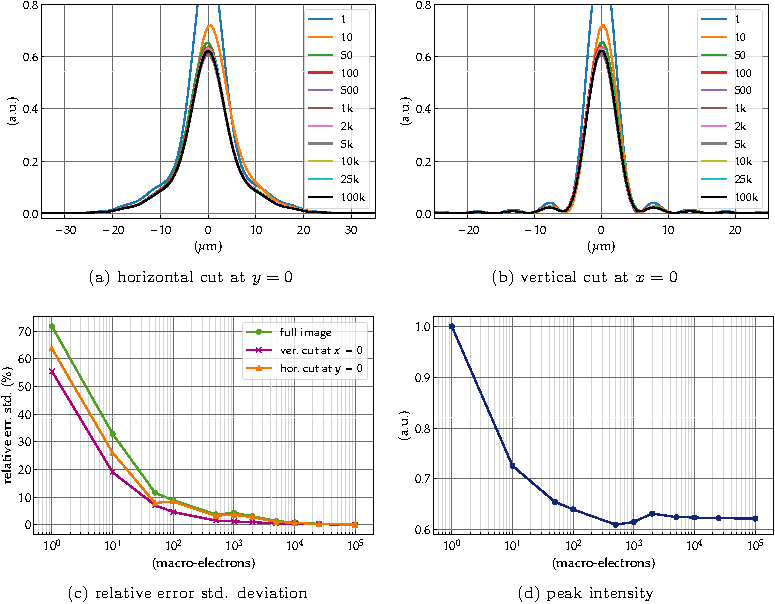
\includegraphics[width=\textwidth]{figures/c1.pdf}
    \caption{Partially-coherent simulations convergence study: case 1. (a) horizontal and (b) vertical intensity cuts at E=7~keV for $me's$ ranging from 1 to 100k. (c) errors relative to the $me's=$100k plots and (d) peak intensity.}
    \label{fig:me_c1}
\end{figure}

\begin{figure}
    \centering
    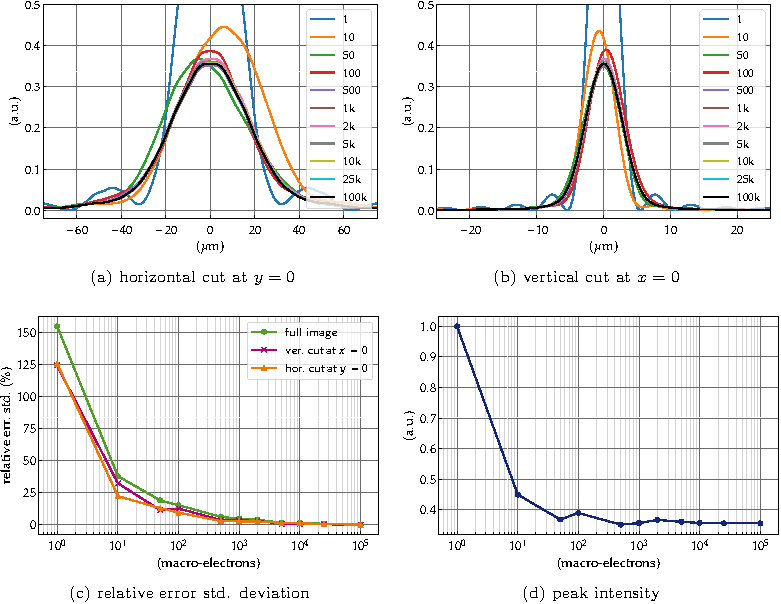
\includegraphics[width=\textwidth]{figures/c3.pdf}
    \caption{Partially-coherent simulations convergence study: case 3. (a) horizontal and (b) vertical intensity cuts at E=7~keV for $me's$ ranging from 1 to 100k. (c) errors relative to the $me's=$100k plots and (d) peak intensity.}
    \label{fig:me_c3}
\end{figure}

\begin{figure}
    \centering
    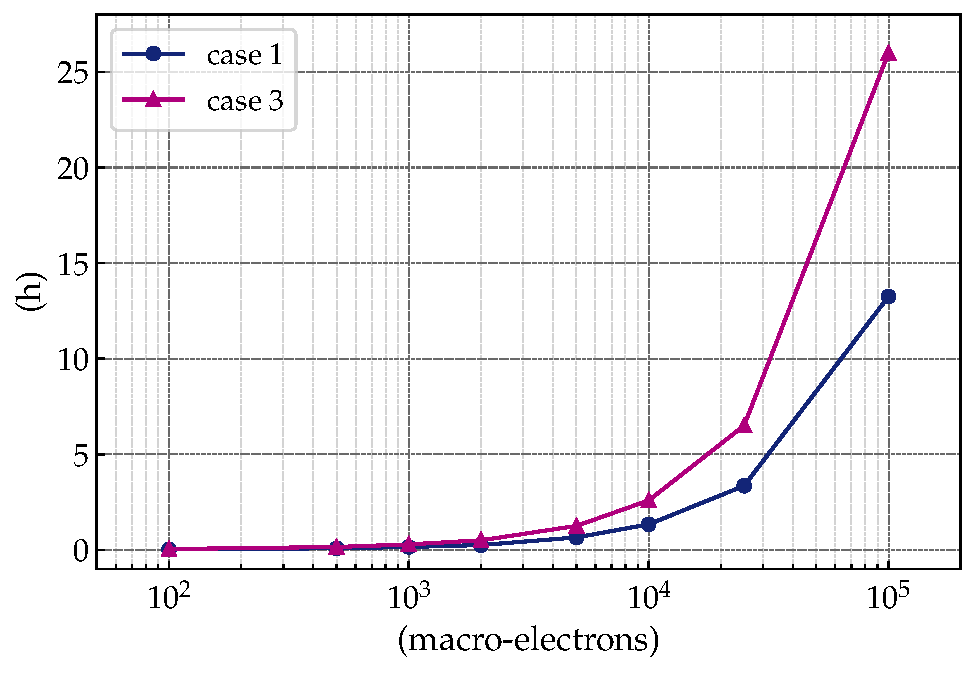
\includegraphics[width=0.8\textwidth]{figures/srw_time.pdf}
    \caption{Total elapsed time for partially-coherent simulations using a computer cluster with 28 processors for parallel calculations as a function of number of $me's$.}
    \label{fig:me_t}
\end{figure}

\newpage
% %%%%%%%%%%%%%%%%%%%%%%%%%%%%%%%%%%%%%%%%%%%%%%%%
% %%%%%%%%%%%%%%%%%%%%%%%%%%%%%%%%%%%%%%%%%%%%%%%%
% %%%%%%%%%%%%%%%%%%%%%%%%%%%%%%%%%%%%%%%%%%%%%%%%

 %-------------------------------------------------------------------------
 % The back matter of the paper - acknowledgements and references
 %-------------------------------------------------------------------------

 % Acknowledgements come after the appendices
\ack{\textbf{Acknowledgements}}

R.C. thanks G. Geloni (EU X-FEL) for the discussion on statistical optics applied to UR in low-emittance storage rings; O. Chubar (NSLS-II/BNL) for the clarifications on selected wavefront propagators; and S. Lordano for sharing information on beamline design for the Sirius light source.

\ack{\textbf{Funding information}}

This project has received funding from the European Union’s Horizon 2020 Research and Innovation programme under grant agreements N$^{\circ}$ 823852 (Photon and Neutron Open Science Cloud -- PaNOSC) and N$^{\circ}$ 101007417 (NFFA-Europe Pilot Joint Activities -- NEP).


%. R.C. acknowledges funding from the European Union’s Horizon 2020 research and innovation programme under grant agreement N$^{\circ}$ 101007417 within the framework of the NFFA-Europe Pilot Joint Activities.




\referencelist{iucr}

 %-------------------------------------------------------------------------
 % TABLES AND FIGURES SHOULD BE INSERTED AFTER THE MAIN BODY OF THE TEXT
 %-------------------------------------------------------------------------

     

\end{document}                    % DO NOT DELETE THIS LINE
%%%%%%%%%%%%%%%%%%%%%%%%%%%%%%%%%%%%%%%%%%%%%%%%%%%%%%%%%%%%%%%%%%%%%%%%%%%%%%






































% %\documentclass[preprint]{iucr}              % DO NOT DELETE THIS LINE
% \documentclass{iucr}              % DO NOT DELETE THIS LINE

% \usepackage{siunitx}
% \usepackage{color}
% % \usepackage{amsmath,amssymb}
% \usepackage{amsfonts} 
% \usepackage{mathtools}
% \usepackage[normalem]{ulem}

% % rotation table labels...
% % see https://tex.stackexchange.com/questions/98388/how-to-make-table-with-rotated-table-headers-in-latex
% \usepackage{adjustbox}
% \usepackage{array}
% \usepackage{booktabs}
% \usepackage{multirow}
% \usepackage{enumitem}

% \newcommand{\todo}[1]{{\color{red}[TODO: "#1'']}}
% \newcommand{\inblue}[1]{{\color{blue}#1}}
% \newcommand{\inred}[1]{{\color{red}#1}}
% \newcommand{\ingreen}[1]{{\color{green}#1}}
% \newcommand{\soutred}[1]{{\color{red}\sout{#1}}}
% \newcommand{\lambdabar}{{\mkern0.75mu\mathchar '26\mkern -8.2mu\lambda}}

% \definecolor{JSR_blue}{RGB}{51, 102, 154}
% \newcommand{\jsrblue}[1]{\textcolor{JSR_blue}{#1}}

% \newcolumntype{R}[2]{%
%     >{\adjustbox{angle=#1,lap=\width-(#2)}\bgroup}%
%     l%
%     <{\egroup}%
% }
% \newcommand*\rot{\multicolumn{1}{R{90}{1em}}
% %
% }
% \journalcode{S}


% \begin{document}                  % DO NOT DELETE THIS LINE

% % \title{Focusing partially-coherent x-ray beams with lenses. Multi-optics simulations}
% \title{A fast and light tool-set for partially-coherent beamline simulations in 4$^{\text{th}}$ generation storage rings based on coherent mode decomposition}    %RC211202: suggestion of new name

% \cauthor[]{\jsrblue{Manuel}}{\jsrblue{Sanchez del Rio}}{srio@esrf.eu}{address if different from \aff}
% \author[]{\jsrblue{Rafael}}{\jsrblue{Celestre}}
% \author[]{\jsrblue{Juan}}{\jsrblue{Reyes-Herrera}}
% \author[]{\newline \jsrblue{Philipp}}{\jsrblue{Brumund}}
% \author[]{\jsrblue{Marco}}{\jsrblue{Cammarata}}

% \aff[]{ESRF - The European Synchrotron, 71 Avenue des Martyrs, 38000 Grenoble, \country{France}}

% \maketitle                        % DO NOT DELETE THIS LINE

% % -----------------------------------------------------------------
% % -----------------------------------------------------------------

% \begin{synopsis}
% Simulations of focusing partial coherent beams with x-ray lenses are performed with different software packages (ShadowOui, SRW, COMSYYL and WOFRY). The four codes give comparable results, that are discussed in detail. 
% \end{synopsis}

% % -----------------------------------------------------------------
% % -----------------------------------------------------------------

% \begin{abstract}
% We simulate the focusing of the radiation produced by fourth-generation storage rings with multiple optics packages implementing a variety of methods for dealing with partial coherence. Ray-tracing uses a hybrid algorithm combining geometrical optics with wave optics corrections. Other codes propagate a set of wavefronts describing the undulator emission. A Monte-Carlo method combine wavefronts from electrons entering to the undulator with different values. Two packages perform coherent mode decomposition of the undulator radiation in 1D and 2D dimensions. The four codes give comparable results for four different setups of an optical system composed by a slit and two beryllium lenses.
% \end{abstract}

% % -----------------------------------------------------------------
% % -----------------------------------------------------------------

% \section{Introduction}
% \label{sec:introduction}

% \todo{re-adequate the introduction to reflect the new direction of the manuscript} 

% Diffraction effects produced when propagating x-ray beams along beamline components are fundamental for the 
% recent fourth-generation storage-ring-based X-ray synchrotron sources. The transverse coherence of these beams is highly improved, in particular in the horizontal direction, with respect to previous 3$^{\text{rd}}$ generation sources.
% Preserving wavefront quality requires better quality materials and optical surfaces in the active beamline components such as mirrors, gratings, crystals and lenses \cite{Yabashi, Roth2017}.

% The effect of radiation coherence is evident in the new synchrotron sources. For example, in case of a focusing system made by a mirror or lens that focuses the source into the image plane. If the numerical aperture (NA) is reduced (for example by the finite dimension of the lens, mirror or by using a slit upstream from the lens) the position and dimensions of the focused beam are altered due to diffraction. This is relevant for synchrotron beamlines, as demonstrated by \citeasnoun{westfahl}, who noticed a shift of the horizontal focal position upstream from the position given by geometrical optics (see Fig. 7 in \citeasnoun{westfahl}) when the horizontal acceptance is reduced by a slit. Their numeric results from wavefront propagation using SRW \cite{codeSRW} including partial coherence agree with an analytical Gaussian Shell-model.

% The diffraction effects in synchrotron radiation cannot be simulated by the limiting cases of full incoherence (usually simulated by geometrical ray-tracing) or by propagating a single wavefront, valid for fully coherent radiation. The coherent fraction of the radiation emitted by new generation storage rings, although much improved with respect to previous generations, is still of the order of a few per cent at hard x-rays. This imply that none of geometrical optics of coherent wavefront propagation describe correctly the beam transport along a typical beamline. Partial coherence should be taken into account, complicating the simulation processes. In the last years several approaches have demonstrated to work for beamlines using undulator radiation. Starting from incoherent beams, \citeasnoun{codeHYBRID} proposed some correction algorithms to include diffraction effects that happen with coherent radiation. More accurate methodologies start from coherent wavefront propagation. The partial coherence is included by propagating a set of wavefronts that all together describe the undulator radiation. Two approaches are possible: calculating the wavefronts emitted by electrons entering in the undulator with different initial conditions, sampled by Monte Carlo from the electron beam emittance (multi-electron in SRW) \cite{codeSRW_ME}, and assigning these wavefronts to the coherent modes, eigenfunctions numerically obtained from making a coherent mode decomposition of the undulator source \cite{codeCOMSYL}.  

% In this paper we study the propagation of a partial coherent beam in the context of the project for the new ID18 beamline at the upgraded EBS-ESRF storage ring. We have compared results for different setups composed by two refractive systems (transfocators), plus a slit placed upstream from the transfocators. The focal spots produced by four different transfocator configuratiuons are studied in detail using four packages: i) hybrid ray-tracing as described by \citeasnoun{codeHYBRID} and implemented in ShadowOUI \cite{codeSHADOWOUI}; ii) multi-electron simulations as implemented in SRW \cite{codeSRW}; iii) full coherent mode decomposition (CMD) in 2D made by the code COMSYL \cite{codeCOMSYL} and then propagated using WOFRY \cite{codeWOFRY}; and iv) a novel 1D coherent mode decomposition also implemented in WOFRY, and based on the previous method but allowing interactive simulations. 

% % To study the performances of such systems a new algorithm for coherent mode decomposition (CMD) of the undulator beams has been developed. This method is very fast allowing parametric simulations in a common laptop.

% % The high efficiency of the CMD software developed is obtained by implementing a 1D model, therefore studying separately the horizontal and vertical planes. 

% % Simulation of the source include coherent mode decomposition (CMD) using COMSYL \cite{codeCOMSYL}, or Monte-Carlo multi-electron propagation with SRW \cite{codeSRW}. It is also found that ray-tracing simulations using the ``hybrid" method \cite{codeHYBRID} give good approximations to the correct results for these systems. A simplified algorithm for CMD in 1D is available in WOFRY. It is very fast allowing parametric simulations in a common laptop, with results in good agreement with the other methods that require a computing cluster.

% % The paper is organized as follows. Section~\ref{sec:theory} summarizes the methodology used for 1D coherent mode decomposition of undulator beams and their transport along the beamline. Section~\ref{sec:onelens} analyzes the focusing of partially-coherent beams with a single refractive system (lens). Section~\ref{sec:twolenses} discusses the pairing of two refractive systems. Section~\ref{sec:complete-beamline} shows simulations for the full beamline and compares different methodologies for a selected case. We finish with a general discussion in Section~\ref{sec:discussion} and  concluding remarks in Section~\ref{sec:summary}. 

% % -----------------------------------------------------------------
% % -----------------------------------------------------------------

% \section{Methods for describing partial coherent beams from undulators in a storege ring}\label{sec:part_coh}
%  \newline
% In this section we present four methods used for dealing with partially-coherent x-ray beams emitted by undulators in low-emittance storage rings. Three of those are already-established methods:  hybrid ray-tracing in ShadowOUI; Monte Carlo multi-electron simulations as implemented in SRW; and the 2D-CDM method implemented in COMSYL. Despite being independently maintained and distributed projects, these are conveniently grouped together within the OASYS suit \cite{codeOASYS} and hence their choice for benchmarking. The fourth approach is the proposed 1D-CMD method separating the horizontal- and vertical-directions implemented in WOFRY, which is also featured in OASYS.


% % We introduce the different methods used for dealing with partially-coherent beams emitted by undulators in low-emittance storage rings: hybrid ray-tracing in ShadowOUI, Monte Carlo multi-electron simulations as implemented in SRW, and CMD, as implemented in COMSYL (2D) and WOFRY (1D). 
% % The use of pure ray-tracing methods (based in geometrical optics) is not adequate when analyzing optical systems dealing with coherent beams (originating diffraction effects). Conventional ray-tracing does not reproduce the effects of focal position shift and focus degradation when the NA is reduced. However, ray-tracing-based methods are much simpler and fast than wave-optics-based methods and in many occasions they are very useful to evaluate the impact of the beam coherence when studying a synchrotron beamline. Because of that, a hybrid \cite{codeHYBRID} algorithm has been developed, incorporating concepts of coherent diffraction in the ray-tracing code SHADOW \cite{codeSHADOW}. It is fully integrated in the ShadowOUI \cite{codeSHADOWOUI} add-on in OASYS. It has been demonstrated to be an efficient and fast tool to design beamlines also including coherence effects. The hybrid ray-tracing can reproduce the effect of degradation of the focus shift and focal shift when changing the NA. 


% \subsection{Multi-electron Monte Carlo (SRW-ME)}
% % ==========================================
% % change the integral (Eq. 1) to the summation and remove the f(r,s,\gamma) - how it is really done & add the intensity normalisation.

% % attention when using Gaussian statistics: make sure the reader understands we do not say UR is Gaussian

% % marks thesis: Eq. in §3.3.1 (Eq. 3.51)

% % PySRU for WOFRY electric field calculation.

% % calculate the coherence length from the FWHM of the first mode and with SRW (x1-x2/2 vs x1+x2/2)- compare both of them. 

% % common introduction to wave optics

% % hybrid send to the end
% % ==========================================

% % SRW~\cite{codeSRW} is a well-established code in the synchrotron community for simulating the emission of synchrotron sources and propagating it along a full beamline. It can be used in single-electron (also called filament beam mode or simply SRW-SE) mode, where the source is the fully coherent undulator radiation in an ideal storage ring with zero emittance. To include finite-emittance, and therefore the production and propagation of partial coherent beams, SRW uses the multi-electron (macro-electrons algorithm or SRW-ME) algorithm, that propagates many wavefronts each one created by an electron that enters in the ID with different initial conditions (position and direction) that are sampled from the parameters of the electron beam (moments or Twiss parameters) using a Monte Carlo method \cite{codeSRW_ME}. This method allows to produce accurate intensity maps (by adding the intensity of individual electrons) and is possible to calculate other parameters of the partially-coherent-beam, such as coherence lengths. The SRW-ME requires the use of HPC. 
% % However, it is not able to store the 4D CSD nor to calculate the CF. 

% In the frequency domain, the synchrotron radiation intensity from $N_\text{e}$ electrons circulating in a storage ring is given by: 
% \begin{equation}
% \begin{split}
% |E&_{\omega\text{~bunch}}(\textbf{r})|^2 \approx \\
%  &N_\text{e} \int\big| E_\omega(\textbf{r};\textbf{s}_\text{e}, \textbf{s}'_\text{e}, \gamma_\text{e})\big|^2 f(\textbf{s}_\text{e}, \textbf{s}'_\text{e}, \gamma_\text{e})~ \text{d}\textbf{s}_\text{e} \text{d}\textbf{s}'_\text{e} \text{d}\gamma_\text{e}~+\\
% &+~ N_\text{e}(N_\text{e}-1)\bigg| \int E_\omega(\textbf{r};\textbf{s}_\text{e}, \textbf{s}'_\text{e}, \gamma_\text{e}) f(\textbf{s}_\text{e}, \textbf{s}'_\text{e}, \gamma_\text{e})~ \text{d}\textbf{s}_\text{e} \text{d}\textbf{s}'_\text{e} \text{d}\gamma_\text{e} \bigg|^2,
% \end{split}
% \label{eq:SR}
% \end{equation}
% where $E_{\omega\text{~bunch}}(\textbf{r})\equiv E_{\text{~bunch}}(x,y;\omega)$ and $E_\omega(\textbf{r})\equiv E(x,y;\omega)$; $\textbf{s}_\text{e}=(x_\text{e},y_\text{e},z_\text{e})$ represents the electron initial positions, $\textbf{s}'_\text{e}=(x'_\text{e},y'_\text{e})$ gives the electron initial directions and $\gamma_\text{e}$ is the electron energy subjected to the energy spread $\delta \gamma_\text{e}$, which have Gaussian distribution in a 6-dimensional space \cite{codeSRW_CSR}. The methods for computing the spontaneous emission by a relativistic electron ($E_\omega$) with initial conditions given by $(\textbf{s}_\text{e}, \textbf{s}'_\text{e},\gamma_\text{e})$ and submitted to an arbitrary magnetic field are described in \cite{Chubar1995,codeSRW}. The first term in the sum from Eq.~\ref{eq:SR} describes temporally incoherent SR and the second term models temporally coherent SR: $\text{I}_\text{~bunch} = \text{I}_\text{~iSR}+\text{I}_\text{~cSR}$. For emitted wavelengths shorter than the electron bunch length, the power associated with the term $\text{I}_\text{~cSR}$ vanishes quickly \cite{Wiedemann2015}.
% Considering typical undulator radiation emission, i.e. x-ray energy ranges from a few hundred electron-volts to a few hundred keV, and typical electron bunch lengths in storage rings ($\sigma_{T}>30$~ps), $\text{I}_\text{~cSR}$ can be neglected when considering standard monochromatisation schemes in beamlines. A further simplification to Eq.~\ref{eq:SR} is done when considering that the intensity of the single-electron emission is not dependent on the initial electron position $z_\text{e}$. The integration of Eq.~\ref{eq:SR} can then be done in 5 dimensions.

% Synchrotron radiation emitted by undulators in storage rings is a fundamentally random process and should be treated probabilistic. The SRW-ME algorithm used to account for partial coherence implements Eq.~\ref{eq:SR} by individually calculating the SR emission of several electrons subjected to the initial conditions sampled from $f(\textbf{s}_\text{e}, \textbf{s}'_\text{e}, \gamma_\text{e})$ assuming these are uncorrelated and passing through an arbitrary magnetic field describing the x-ray source. Each resulting electric field from this Monte-Carlo sampling is then propagated through the beamline until the observation point, where the contributions from different electrons are added in intensity as stated in Eq.~\ref{eq:SR} \cite{codeSRW_ME}. It is impractical (and unnecessary) to account for the emission of every single electron in a beam that very often has a current of few hundreds mA. Electrons are then divided in so-called macro-electrons (\textit{me's}), which is an abstraction that allows to group the emission of several individual electrons into one particle behaving (in electro-dynamics theory terms) as a single electron emission, but with resulting intensity given by the total intensity $\text{I}_\text{~bunch}$ divided by the number of macro-electrons used in the simulation. An advantage of the SRW-ME approach is that the electric fields of the \textit{me's} propagate independently from each other, which allows a convenient parallelisation of the wavefront propagations among many processors. Indeed, SRW-ME calculations require the use of HPC in most cases.

% % we developed a 1D model of the CMD method that we previously developed in 2D \cite{glass2017}. The motivation for developing these new tools is to perform quick calculations (e.g., being able to perform parametric calculations in a laptop) with high accuracy in the simulation of the source and beam propagation. The separation of the real 2D wavefront in two separated 1D wavefronts is well justified for most synchrotron beamlines, where the cross-talk between these two directions is small. 
% % The tools developed here are included in the OASYS toolbox \cite{codeOASYS}, available as an WOFRY add-on. These tools can be used from the OASYS interface, which also creates scripts that can be later modified for performing parametric calculations and loops in batch runs. 


% \subsection{Coherent mode decomposition of undulator radiation in a storage ring}
% % \subsection{Coherent mode decomposition of undulator radiation in a storage ring (COMSYL)}
% %The electrons in a storage ring are statistically distributed, following in good approximation a Gaussian distribution in a 6-dimensional space (three spatial coordinates, two angles to define direction, and the electron energy). The radiation of the individual electrons will add incoherently for wavelengths smaller than the bunch lengths. This is the usual case for X-rays produced by storage ring-based sources, but not for free electron lasers. Therefore, each electron creates a wavefront (fully coherent) associated at a given photon energy. As a consequence, the overall radiation cannot be described deterministically. Statistical methods are then needed, like for describing the electron beam. This is the origin of partial coherence of the synchrotron emission. In an ideal storage ring of zero emittance, the electrons follow a filament beam so the emission by an insertion device (ID) would be fully coherent. When electron emittance is considered, the electrons contributing to the radiation have different initial conditions (in the 6-dimensional space) and the overall emission cannot be describe by a single wavefront, but by statistically distributed wavefronts, described by partial coherent optics.

% %The radiation is ``wide sense stationary" \cite{mandel_wolf} if it verifies some conditions, usually satisfied for light emitted by storage rings, but not for XFELs \cite{geloni2008}. These conditions can be summarized as
% %i) the electron bunch length being long enough (several times larger than the emitted wavelength),
% %ii) radiation is monochromatized 'not too much' (like by standard monochromators), and 
% %iii) the radiation frequency being large enough.
% %It is in this case all the coherent properties of the radiation can be described using $W$, the ``cross spectral density" (CSD), a complex function that measures the correlation of the electric field $E$ in two different spatial points at a given radiation frequency $\omega$. It can be mapped in a $(x,y)$ plane at a third coordinate $z$. At that plane, the CSD depends on 5 variables: 

% % \begin{equation}
% % W_{2D}(x_1,y_1,x_2,y_2;\omega) = <E^*(x_1,y_1;\omega) E(x_2,y_2;\omega)>
% % \label{eq:CSD_1D}
% % \end{equation}
% % The modulus of the complex degree of coherence is one for a completely coherent beam and zero for an incoherent beam. 

% % An important result in partial coherence optics permits to describe the radiation as an infinite sum of independent coherent modes (in the sense of orthonormality) :
% % \begin{equation}
% % W_{2D}(x_1,y_1,x_2,y_2,\omega) = \sum_{n=0}^{\infty} \Lambda_n(\omega) \Phi_{n}^*(x_1,y_1,\omega) \Phi_{n}(x_2,y_2,\omega) 
% % \label{CMD}
% % \end{equation}
% % where $\Lambda_n$ (eigenvalues) are the intensity weights and the $\Phi$ are the coherent modes (eigenfunctions). 
% % Some important characteristics of this coherent mode decomposition are: i) the modes are orthonormal (in the integral sense), ii) the modes maximize the spectral density, the first mode is more intense than the second, and so on, meaning that the truncated expansion is optimal, and iii) there is complete coherence if and only if there is only a single mode. If one can truncate the infinite series to a limited number of modes $N$ which contain a good percentage of the spectral density, the numerical storage of the $N$ modes that depend on two spatial variables is usually more economic than the storage of the cross spectral density $W$ that depends on four variables. 
% % The eigenvalues $\Lambda_n$ are a measure of the intensity. One can define the occupation $\eta$ of the i-th mode as the normalized intensity: 

% % \begin{equation}
% % \eta_i(\omega) = \frac{\Lambda_i(\omega)}{\sum_{n=0}^{\infty} \Lambda_n(\omega)}
% % \end{equation}

% % From these arguments, it is now natural to rigorously define Coherent Fraction ($CF_{2D}$) as the occupation of the first coherent mode: $CF_{2D}=\eta_0$.

% % %%%%%%%%%%%%%%%%%%%%%%%%%%%%%
% % The interest of the coherent mode decomposition method is twofold: the possibility to propagate a partial coherent beam along the beamline by just propagating a few modes (less modes for a more coherent beam) which behave like coherent wavefronts, and the use of the coherent fraction (a scalar parameter) as a well-defined measure of how coherent is the beam at any position of the beamline.

% \citeasnoun{geloni2008} show that although SR emission (a random process obeying Gaussian statistics) is not intrinsically stationary nor homogeneous, second order coherence theory of scalar fields as presented by \citeasnoun{mandel_wolf} can be applied if the following conditions are observed:
% \begin{enumerate}[label=(\roman*)]
% \item radiation frequency $\omega$ is ``sufficiently high";
% \item $e^-$ bunch length $\sigma_{T}$ ``sufficiently large" so that $\omega\sigma_{T}\gg1$;
% \item radiation bandwidth $\Delta_\omega$ is not ``too narrow" ($\Delta_\omega\gg1/\sigma_{T}$).
% \end{enumerate}
% Basically excluding infra-red downwards, condition (i) holds for soft- to hard x-rays, which are upwards in frequency; condition (ii) is satisfied by storage rings, where typically $\sigma_{T}>30$~ps, but not at free-electron lasers, where $\sigma_{T}<0.1$~ps due to micro-bunching effects; and finally, condition (iii) is generally met by standard\footnote{\citeasnoun{geloni2008} provide a counter-example in Ref[15] ibid.} monochromatisation schemes.
% This set of conditions ensures that SR emission is a quasi-stationary (or wide-sense stationary) process. Other two necessary conditions, these related to quasi-homogeneity, are implicitly met when:
% \begin{enumerate}[label=(\roman*)]
% \setcounter{enumi}{3}
% \item $N_\text{x}\gg1$ and $D_\text{x}\gg1$;
% \item $N_\text{y}\gg1$ and/or $D_\text{y}\gg1$,
% \end{enumerate}
% with:
% \begin{equation*}
%     N_\text{x,y}=\frac{\sigma^2_\text{x,y}}{\lambdabar L_u}, \quad D_\text{x,y}=\frac{\sigma'^2_\text{x,y}}{\lambdabar/L_u}
% \end{equation*}
% where $\sigma_\text{x,y}$ and $\sigma'_\text{x,y}$ represent the electron beam transverse sizes and divergences, $L_u$ is the undulator length (number of periods $N_u$ times the magnetic period $\lambda_u$) and $\lambdabar=\lambda/2\pi$. Conditions (iv) and (v) are met for the wavelengths already restricted by (i). As noted by \citeasnoun{geloni2008}, the conditions imposed are practically non-restrictive under cases of practical interest.

% When the aforementioned restrictions are respected, the cross-spectral density (CSD) can be used to completely describe a partially-coherent field from the statistical-optics framework. At any position \textit{z} in a beamline, including at the source, the cross-spectral density \textit{W} can be written as:
% \begin{equation}
% W_\text{2D}(\textbf{r}_1,\textbf{r}_2;\omega) = \big\langle E^*(\textbf{r}_1;\omega)  E(\textbf{r}_2;\omega)\big\rangle,
% \label{eq:CSD_2D}
% \end{equation}
% where $\bullet^*$ indicates the complex conjugate, the averaging brackets $\langle \bullet \rangle$ indicate average over the bunches, $\textbf{r}_1=(x_1,y_1,z)$ and $\textbf{r}_2=(x_2,y_2,z)$. It is also useful to define the spectral density\footnote{Which is sometimes loosely called intensity. The spectrum density and the intensity functions are equivalent for the quasi-monochromatic case. The same holds for the CSD and the mutual optical intensity (MOI) \cite{mandel_wolf}.} for the case where $\textbf{r}=\textbf{r}_1=\textbf{r}_2$ as $I(\textbf{r};\omega)=W_\text{2D}(\textbf{r},\textbf{r};\omega)$. We also define the normalised cross-spectral density function or spectral degree of coherence (SDC):
% \begin{equation}
% \mu(\textbf{r}_1,\textbf{r}_2;\omega) = \frac{W_\text{2D}(\textbf{r}_1,\textbf{r}_2;\omega)}{\sqrt{I(\textbf{r}_1;\omega) I(\textbf{r}_2;\omega)}}.
% \label{eq:DTC}
% \end{equation}
% The absolute value of Eq.~\ref{eq:DTC} is limited: $0\leq|\mu(\textbf{r}_1,\textbf{r}_2;\omega)|\leq 1$, where $|\mu|=0$ means total uncorrelation and $|\mu|=1$ denotes full correlation of the fluctuations at positions $\textbf{r}_1$ and $\textbf{r}_2$.

% A well known result from coherence theory is the coherent mode representation of partially coherent fields in free-space - see §4.7.1 in \cite{mandel_wolf}. It is possible to decompose the CSD in a infinite sum of orthonormal coherent modes:
% \begin{equation}
% W_\text{2D}(\textbf{r}_1,\textbf{r}_2;\omega) = \sum_{n=0}^{\infty} \Lambda_n(\omega) \Phi_{n}^*(\textbf{r}_1;\omega) \Phi_{n}(\textbf{r}_2;\omega) 
% \label{eq:CMD}
% \end{equation}
% where $\Lambda_n$ (eigenvalues) are the intensity weights and the $\Phi$ are the coherent modes (eigenfunctions). 
% Some important characteristics of this coherent mode decomposition are: 

% \begin{enumerate}[label=(\roman*)]
% \item the modes $\Phi$ are orthonormal in the integral sense;
% % \end{enumerate}
% % \begin{equation*}
% % \int W_\text{2D}(\textbf{r}_1,\textbf{r}_2;\omega)  \Phi_{n}(\textbf{r}_1;\omega)~ \text{d}\textbf{r}_1 = \Lambda_n(\omega) \Phi_{n}(\textbf{r}_2;\omega);
% % % \label{eq:orthonormal_modes}
% % \end{equation*}
% % \begin{enumerate}[label=(\roman*)]
% % \setcounter{enumi}{1}
% \item the modes maximize the CSD making the truncation optimal:
% \end{enumerate}
% \begin{equation*}
% \Lambda(\omega) \in \mathbb{R}
% :~0\leq \Lambda_{i+1}(\omega)<\Lambda_i(\omega);~\forall~i \in \mathbb{N};
% \end{equation*}
% \begin{enumerate}[label=(\roman*)]
% \setcounter{enumi}{2}
% \item the eigenvalues $\Lambda_n$ are a measure of the intensity of the corresponding mode $\Phi_{n}$; 
% \item we define the occupation $\eta$ of the i-th mode as the normalized intensity: 
% \begin{equation}
% \eta_i(\omega) =\frac{\Lambda_i(\omega)}{\sum\limits_{n=0}^\infty{\Lambda_n(\omega)}};
% \end{equation}
% \item radiation is considered fully-coherent if and only if there is only a single mode.
% \end{enumerate}

% From these arguments, it is now natural to rigorously define coherent fraction ($\text{CF}_\text{2D}$) as the occupation of the first coherent mode:
% \begin{equation}
% \text{CF}_\text{2D}=\eta_0=\frac{\Lambda_0(\omega)}{\sum\limits_{n=0}^\infty{\Lambda_n(\omega)}}. \label{eq:CF2D}
% \end{equation}
% When using Eq.~\ref{eq:CF2D}, it is relevant to consider that if there is spatial filtering or any sort of beam clipping the modes $\Phi$ do not propagate retaining their orthogonality and their occupation $\eta$. In this case, a reapplication of the CMD to the cropped modes (rediagonalisation) is imperative to recalculate the new $\text{CF}_\text{2D}$.

% We also define the transverse coherence length (CL) based on the width of the first mode $\Phi_0$, acknowledging issues with this definition arising mainly from the fact that here is no unanimous accepted way of defining the beam width. However, given the importance of such parameter for daily beamline operations (eg. choosing slit sizes) and that blindly applying the van-Cittert-Zernike (VCZ) theorem may lead to errors - cf. §4.1 in \cite{geloni2008}, we decided to put the CL on a firmer footing. This definition holds for both horizontal directions and is dependent on the criteria used for defining the beam width along that direction. % \todo{a possible new section describing the coherent parameters (CF, coherent length, etc) and the way to obtain them via rediagonalization...}

% The interest of the coherent mode decomposition method in optical design of x-ray beamlines is manyfold: the possibility of propagating a partially-coherent beam along a beamline by just propagating a few hundred modes which behave like coherent wavefronts as opposed to a few thousand wavefronts when doing multi-electron Monte-Carlo simulations; the use of the coherent fraction (a scalar parameter) as a well-defined measure of how coherent is the beam at any position of the beamline; and if one can truncate the infinite series to a limited number of modes $N$ which contain a good percentage of the spectral density, the numerical storage of the $N$ modes that depend on two spatial variables is usually more economic than the storage of the cross spectral density $W$ that depends on four variables. 

% \subsubsection{COherent Modes for Synchrotron Light (COMSYL)} .
%  \newline

% \todo{Manolo: explain how the CSD is calculated; how the CMD is done and how the rediagonalisaiton can be done. Refer to \cite{codeCOMSYL} and \cite{glass2017}. One should also say that COMSYL wavefronts can be propagated with SRW and WOFRY - link to chapter 3}.

% \begin{equation}
% \begin{split}
%     W_\text{2D}&(\textbf{r}_1,\textbf{r}_2;\omega) = \\
%     &\int E_\omega^*(\textbf{r}_1;\textbf{s}_\text{e}, \textbf{s}'_\text{e}, \gamma_\text{e}) E_\omega(\textbf{r}_2;\textbf{s}_\text{e}, \textbf{s}'_\text{e}, \gamma_\text{e})f(\textbf{s}_\text{e}, \textbf{s}'_\text{e}, \gamma_\text{e})~ \text{d}\textbf{s}_\text{e} \text{d}\textbf{s}'_\text{e} \text{d}\gamma_\text{e},
% \end{split}\label{eq:comsyl_CSD}
% \end{equation}

% \subsubsection{1D coherent mode decomposition: separate horizontal and vertical directions (WOFRY)} .
%  \newline

% % In the following, we suppose that the CSD is separable in its 1D horizontal $x$ and vertical $y$ coordinates, therefore the $W_{2D}$ becomes a product of two CSD functions $W$ of two variables for a given photon frequency $\omega$:

% % \begin{equation}
% % W_{2D}(x_1,y_1,x_2,y_2;\omega) = W(x_1,x_2;\omega) W(y_1,y_2;\omega).
% % \label{eq:CSD_2D_bis}
% % \end{equation}
% % Each $W$ function is treated separately in a similar way affecting the $x$ (horizontal) and $y$ (vertical) coordinate. This separation is believed to work well for non-round beams, and for photon energies not far from the undulator resonance \cite{tanaka2014,nash2021}. The CMD for each direction is:
% % \begin{equation}
% % W(x_1,x_2;\omega) = \sum_{n=0}^{\infty} \lambda_n(\omega) \phi_n^*(x_1;\omega) \phi_n(x_2;\omega) 
% % \label{eq:CMD1D}
% % \end{equation}
% % with $\lambda_n$ the 1D eigenvalues and $\phi_n$ the 1D eigenfunctions. This gives raise to two values of coherence fraction, for the horizontal and vertical directions, and the 2D CF is the product $CF_{2D}=CF_H \times CF_V$. The $\phi_n$ eigenvectors can be are propagated to any position of the beamline like standard wavefronts. Calling $\phi'$ the wavefront originated by propagating the (source) mode $\phi$, we can construct the propagated CSD    
% % \begin{equation}
% % W'(x_1,x_2;\omega) = \sum_{n=0}^{\infty} \lambda_n(\omega) \phi'^{*}_n(x_1;\omega) \phi'_n(x_2;\omega).
% % \label{eq:propagatedCSD}
% % \end{equation}
% % Note that the propagated wavefronts $\phi'$ are in general not orthonormal therefore there are not coherence modes. A new CMD of $W'$ must be done to calculate new eigenvalues and eigenvectors (modes) and the propagated CF. The propagated wavefronts in (equation~\ref{eq:propagatedCSD}) are orthonormal only in the cases of free propagation in vacuum and ideal focusing. Any element that crop the beam or include absorption imply that propagated wavefronts $\phi'_n$ are not longer orthonormal.  

% We now suppose that the CSD (Eq.~\ref{eq:CSD_2D}) can be written as a product of a horizontal- and a vertical cross-spectral densities: 
% \begin{equation}
% W_\text{2D}(\textbf{r}_1,\textbf{r}_2;\omega) = W_\text{1D}(x_1,x_2;\omega)W_\text{1D}(y_1,y_2;\omega).
% \label{eq:CSD_2D_bis}
% \end{equation}
% \begin{equation}
% W_\text{2D}(\textbf{r}_1,\textbf{r}_2;\omega) = W_\text{1D}(x_1,0,x_2,0;\omega)W_\text{1D}(0,y_1,0,y_2;\omega).
% \label{eq:CSD_2D_bis2}
% \end{equation}
% The factorisation in Eq.~\ref{eq:CSD_2D_bis} has been discussed §3.1 from \cite{geloni2008} - see Eq.~56 ibid. In the context of the Wigner distribution, this separation in horizontal and vertical components has been discussed by various authors is believed to work well for photon energies not far from the undulator resonance and for non-round beams \cite{tanaka2014,nash2021}. The CSD and the Wigner distribution being related by a Fourier transform. 

% % In the following, we suppose that the CSD is separable in its 1D horizontal $x$ and vertical $y$ coordinates, therefore the $W_{2D}$ becomes a product of two CSD functions $W$ of two variables for a given photon frequency $\omega$:

%  The CMD for each direction is:
% \begin{equation}
% W(x_1,x_2;\omega) = \sum_{n=0}^{\infty} \lambda_n(\omega) \phi_n^*(x_1;\omega) \phi_n(x_2;\omega) 
% \label{eq:CMD1D}
% \end{equation}
% with $\lambda_n$ the 1D eigenvalues and $\phi_n$ the 1D eigenfunctions. This gives raise to two values of coherence fraction, for the horizontal and vertical directions, and the 2D CF is the product $CF_{2D}=CF_H \times CF_V$. The $\phi_n$ eigenvectors can be are propagated to any position of the beamline like standard wavefronts. Calling $\phi'$ the wavefront originated by propagating the (source) mode $\phi$, we can construct the propagated CSD    
% \begin{equation}
% W'(x_1,x_2;\omega) = \sum_{n=0}^{\infty} \lambda_n(\omega) \phi'^{*}_n(x_1;\omega) \phi'_n(x_2;\omega).
% \label{eq:propagatedCSD}
% \end{equation}
% Note that the propagated wavefronts $\phi'$ are in general not orthonormal therefore there are not coherence modes. A new CMD of $W'$ must be done to calculate new eigenvalues and eigenvectors (modes) and the propagated CF. The propagated wavefronts in (equation~\ref{eq:propagatedCSD}) are orthonormal only in the cases of free propagation in vacuum and ideal focusing. Any element that crop the beam or include absorption imply that propagated wavefronts $\phi'_n$ are not longer orthonormal. 

% \todo{maybe is interesting to explain here how to obtain 2D data by outer product of H and V profiles, something that is used later on}

% \subsection{Hybrid ray-tracing (ShadowOUI)}

% Ray-tracing-based methods are simpler and faster than wave-optics-based methods and more often than not, offer useful insight when studying and designing a synchrotron beamline \cite{hierarchical}. However, the use of pure ray-tracing methods based in geometrical optics are not very adequate when analyzing optical systems dealing with (partially- or fully-) coherent beams subjected to strong diffraction effects - eg. beam clipping by either physical acceptance of an optical element or by slits; and optical errors. To the geometric methods, it is possible to add diffraction effects by convolution of the beam divergence profiles calculated by ray-tracing and by applying the diffraction integrals, then proceeding with classical ray-tracing methods for treating optical elements and free-space propagation. Building on that hybrid concept, an extension to the ray-tracing code SHADOW \cite{codeSHADOW} has been proposed by \citeasnoun{codeHYBRID}, which is fully integrated in the ShadowOUI \cite{codeSHADOWOUI} add-on in OASYS. Since its release, this hybrid ray-tracing implementation has been successfully used as an efficient and fast tool to design beamlines also including coherence effects \cite{Shi2017,Luca2020, Lordano2022}.

% \section{Propagation of wavefronts along the beamline}
%  \newline

% In terms of design using physical optics, an x-ray beamline is composed of two main elements: drift spaces and optical elements. The first class is handled with diffraction integrals and a brief explanation of the wavefront propagators used by the software in section~\ref{sec:part_coh} is presented here. Optical elements can usually be represented by a transmission element, which is also covered in this section. 

% % \subsection{Wavefront propagation in free-space (Drift spaces)}\label{sec:free_space}
% \subsection{Drift spaces}\label{sec:free_space}

% The wavefront evolves when transported in free space from two different positions along the optical axis. Integral propagators are to calculate the wavefront in a given point starting from the wavefront in a previous position. 

% \todo{short paragraph for propagators in SRW - cite \cite{ChubarCelestre} }
% A propagator based on \cite{schmidt} is implemented in WOFRY (both 1D and 2D versions) to calculate the transported field in a ``zoomed'' window. Wofry 1D also implements an ``integral" propagator based on the direct numerical integration of the  Rayleigh-Sommerfeld integral \cite{srioLBL}

% \subsection{Optical elements}\label{sec:OE}

% Transmission element and free-form optics

% Thick elements and Multi-slicing 

% \subsubsection{Apertures, slits and other forms of beam cropping} are

% A generic aperture is a mask that transmits a part of the wavefront complex amplitude in a range $[x_{min},x_{max}]$ and absorbs the rest. It can be
% \begin{equation}
% R(x;\omega) =
% \left\{
% \begin{matrix}
% A,  & \mbox{~~if~~} x_{min} \le x \le x_{max}
% \\ 
% 1 - A, & \mbox{~~elsewhere}
% \end{matrix}
% \right.
% \end{equation}
% When the element is a slit, then $A=1$. If it is a beamstop, then $A=0$. In the following simulations we will use an aperture of finite length $a$ centered with the beam, therefore $x_{min}=-a/2$ and $x_{max}=a/2$.


% \subsubsection{X-ray lenses}

% A refractor made by a material with refraction index $n(\omega)=1-\delta(\omega)+i\beta(\omega)$ 
% and thickness profile $z(x)$ adds a phase to the wavefront $-\lambda \delta(\omega) z(x)$ and reduce its amplitude by $\exp(-\mu z(x)/2)$, where $\mu=(4 \pi/\lambda) \delta(\omega)$ is the (intensity) attenuation coefficient. These expressions can be applied to any transmission object of profile $x(z)$ assuming valid the thin object approximation. 

% The changes induced by a real lens in the wavefront can be calculated using the thin object approximation discussed below, using the lens profile. Usually, a single lens has a parabolic interface $z=x^2/(4R)$ with $R$ the radius at the apex. A lens has two parabolic interfaces (front and back) separated by a lens thickness $d$. The interfaces are flat outside the lens aperture $L$. Therefore, the lens profile is:
% \begin{align}
%     z(x) &= \frac{1}{2R} x^2 + d; & |x| < L/2\\ \nonumber
%     z(x) &= \frac{1}{2R} (L/2)^2 + d; & |x| \ge L/2.
% \end{align}

% A Compound Refractive Lens is a pile of $N$ identical lenses. If we neglect the beam propagation in the inter-lens space, the effect of the $N$ lenses is identical of a single lens with profile $x_N(z)=N z(x)$. If one is interested in assessing the effect of the inter-lens space (e.g. for studying the adiabatic focusing \cite{Schroer_adiabatic}) the CRL must be calculated as $N$ independent lenses, applying the free-space propagator in between two consecutive lenses. For a transfocator (a transfocator is a pile of CRLs) the same concept apply: it is possible to compute the accumulated lens profile and use it as a single lens, or calculate lens by lens (or CRL by CRL) if the effect of inter-lens or inter-CRL spaces are to be taken into account.

% \subsubsection{Mirrors; zone plates, crystals and other diffractive optics} blablabla 


% \section{Description of the optical system}
% \label{sec:beamline}


% The optical system under consideration is based on the future ID18 beamline at ESRF. This will be a long beamline (200 m) for applications exploiting the beam coherence. The source considered is an undulator with period 18 mm and 138 periods (length close to 2.5 m).  
% We analyze a focusing system with two transfocators, at 65 and 170 m from the source. They contain sets of 2D and 1D lenses that will permit modifying independently the focal lengths for the horizontal and vertical directions. The use of two transfocators allows a great flexibility in the beam transport. The first one can be used to modify the divergence of the beam, even to collimate it, to guarantee a full illumination at the second transfocator.  

% The two transfocators in use are idealized as two real beryllium lenses of variable curvature radius $R_1$ and $R_2$ that correspond to focal distances $f_1$ and $f_2$ ($f=R/(2 \delta)$, with $\delta=$~6.96 10$^{-6}$ for Be at \SI{7}{keV}). A slit of aperture $a_h$ in horizontal and $a_v$ in vertical is placed upstream the lens-1. We set the distances matching the requirements of the EBS-ESRF ID18 beamline (see Table~\ref{table:id18parameters}), and we analyzed the system at a photon energy of \SI{7}{keV} for different focal distances of lens-1 and lens-2. 

% % The final goal is to get the desired focal size by selecting the configuration of the transfocators (the focal length and the particular combination of lenses to approach it). 

% \begin{table}[]
%     \label{table:id18parameters}
%     \caption{Position of the two transfocators, slit and sample (focal point) corresponding to the ID18 beamline configuration under study. }
%     \centering
%     \begin{tabular}{l|c|c}
%          element & position [m] & comment\\
%          ID (undulator) source& 0 & U18 $N_u$~=~138 $K$~=~1.851 (7 keV)\\
%          Slit & 36 &
%          variable aperture $a_h\times a_v$
%          \\
%          Transfocator 2D & 65 & 
%          %$f_H=58.7; f_V=54.3$ 
%          \\
%          Transfocator 2D & 170 & $D$~=~\SI{105}{\meter} \\
%         %  Transfocator 2D & 170 & position 1 {\bf FO1}, $D$=~\SI{105}{\meter} \\
%         %  Transfocator 2D & 192 & position 2 {\bf FO2}, $D$=~\SI{127}{\meter}  \\
%          sample & 200 & focal plane
%     \end{tabular}
% \end{table}

% We are interested in the beam properties (intensity distribution, size, flux) at the sample plane for four cases.
% The first case is selected to obtain a small spot (about \SI{5}{\micro\meter}) and the second one a large spot (more than \SI{30}{\micro\meter}). For these cases the slits are selected to match a $CF_h=CF_v=$~90\% for a photon energy of \SI{7}{keV}. The values are shown in Table~\ref{table:2Dusercases}. The cases 3 and 4 follow the same logic but the slits are opened to increase intensity at expensed of reducing coherence  ($CF_h=CF_v=$~70\%). 


% \begin{table}[]
%     \label{table:2Dusercases}
%     \caption{Configurations selected for 2D simulations. Slit aperture ($a_h$ or $a_v$) is selected for obtaining $CF_h=CF_v=$~90\% in cases 1 and 2, and $CF_h=CF_v=$~70\% in cases 3 and 4. 
%     }
%     % \centering
%     \begin{tabular}{c|c|c|c|c|c}
%          case h/v & $a_h/a_v$ [\SI{}{\micro\meter}] & $f_1$ [m] & $f_2$ [m] & $R_1$ [\SI{}{\micro\meter}]& $R_2$ [\SI{}{\micro\meter}] \\
%          \hline
% 1 h &      40.3 & 46.1 &     26.5 &     641.9 &     369.5 
% %&     86
% \\
% 1 v &      227.0 & 15.0 &     22.2 &     209.4 &     309.6 
% % & 21
% \\
% \hline
% 2 h &      40.3 & 25.1 &     21.3 &     349.1 &     296.3  
% % & 42 
% \\
% 2 v &      227.0 & 42.2 &     55.6 &     588.6 &     775.3 
% % &     78
% \\
% \hline \hline
% 3 h &      85.1 & 46.1 &     31.8 &     641.9 &     443.7 
% % &     86 
% \\
% 3 v &      506.7 & 85.2 &     27.8 &     1187.4 &     387.6  
% % &     168 
% \\
% \hline
% 4 h &      85.1 & 25.1 &     20.7 &     349.1 &     288.7 
% % &     42 
% \\
% 4 v &      506.7 & 42.2 &     55.7 &     588.6 &     776.0 
% % &     78 

%     \end{tabular}
% \end{table}


% \section{Results of multi-optics simulations}
% \label{sec:complete-beamline}

% Calculations are done using different methodologies, implemented in four different software codes. 

% We first calculated the illumination at the entrance slit plane. The beam at this position comes from the free propagation of the undulator emission, therefore it has the same coherence fraction as the source. The intensity distribution is shown in Fig.~\ref{fig:intensityat36m}, where the horizontal and vertical profiles calculated by Wofry1D and SRW-ME are compared. The effect of the partial coherence is important: a coherent beam would give very different values \todo{add numbers? repeat the simulations here}. \todo{may be comment 1) that the coherent illumination if different for SRW (zero emittance) than for Wofry1D (zeroth mode), and 2) we could calculate precisely the FWHM values of the profiles and compare with the typical analytical convolution calculation.}   

% \begin{figure}
%     \label{fig:intensityat36m}
%     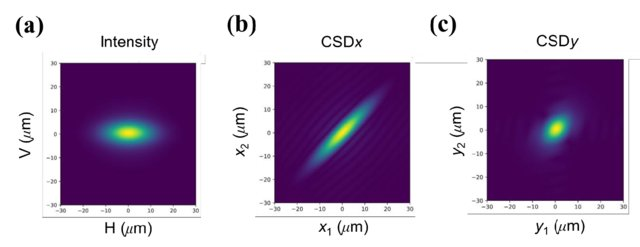
\includegraphics[width=0.99\textwidth]{figures/a-intensity-b-CSDx-and-c-CSDy-of-the-secondary-source_W640.jpg}
%     (d) 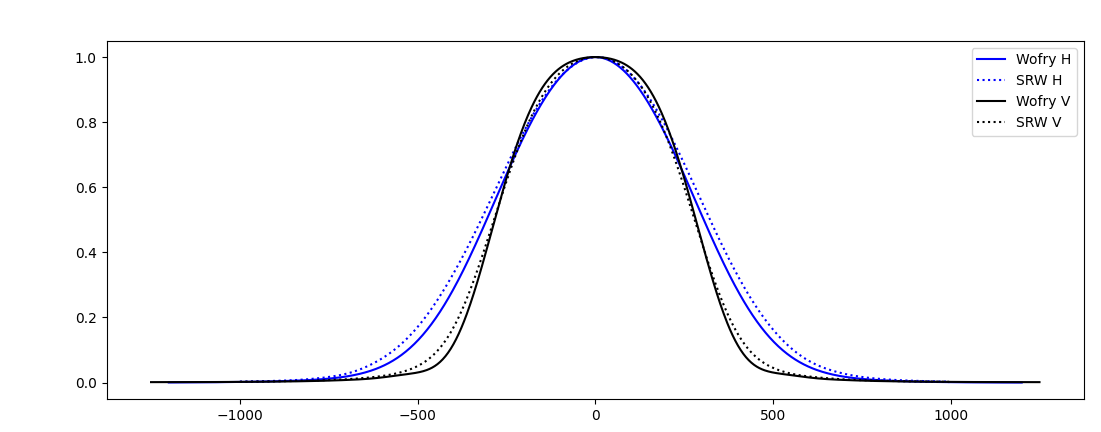
\includegraphics[width=0.75\textwidth]{figures/profiles_at_36m.png}
%     \caption{Intensity (a) and CSD in 1D for H (b) and V (c) directions calculated by \todo{Wofry1D and} SRW-ME  (d) comparison of the central intensity profiles. \todo{redo the figure...}}
% \end{figure}


% The results of intensity distribution at the sample plane are display in Figs.~\ref{fig:hybrid}-\ref{fig:2DWofry1D}, for results using hybrid, SRW, COMSYL and WOFRY1D codes, respectively.  Beam dimensions are obtained by calculating the full width at half maximum (FWHM) from the intensity distrubution at one direction, resulting by integrating the other direction. They are displayed in the plots, and summarized in Table~\ref{table:comparison}.
% The results for case 1 shows an horizontal profile mostly triangular with shoulders that evidence small diffraction fringes. The fringes are more resolved in the vertical direction. Case 2  presents in horizontal a soft Gaussian-like profile, but in vertical important symmetric shoulders are remarked. Case 3 shows a smooth Gaussian profile in horizontal and a small shoulder with fringes in vertical. Case 4 shows a conventional smooth profile in horizontal but an original three-lobe plateau in vertical. This variety of profile distribution demonstrates how relevant the diffraction effects are, which modulate the beam shape in a non-trivial way.  

% \newpage

% \begin{figure}
%     \label{fig:hybrid}
%     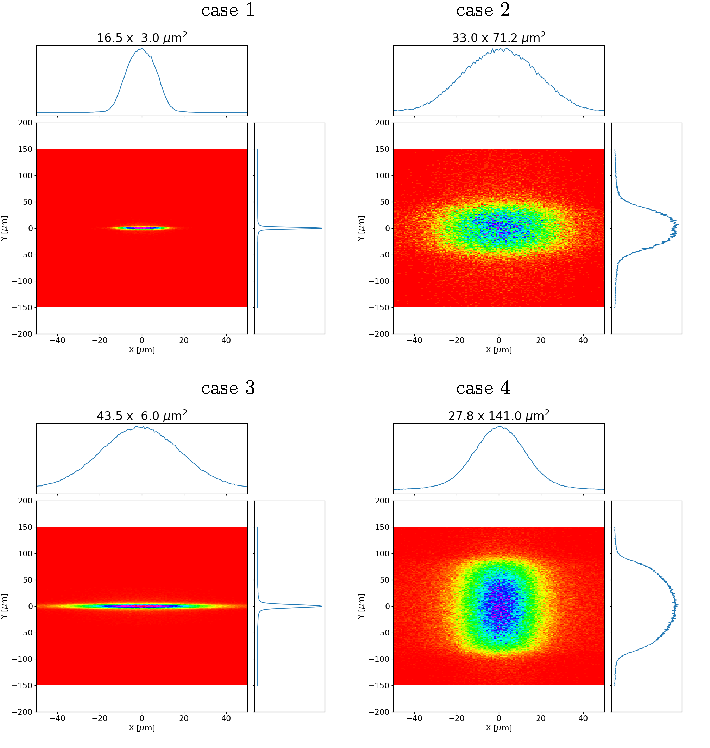
\includegraphics[width=0.99\textwidth]{figures/fig_hybrid.pdf}
%     \caption{Hybrid ray-tracing calculations of the intensity distribution at the focal plane for the cases listed in Table~\ref{table:2Dusercases}.}
% \end{figure}

% \begin{figure}\label{fig:srw}
%     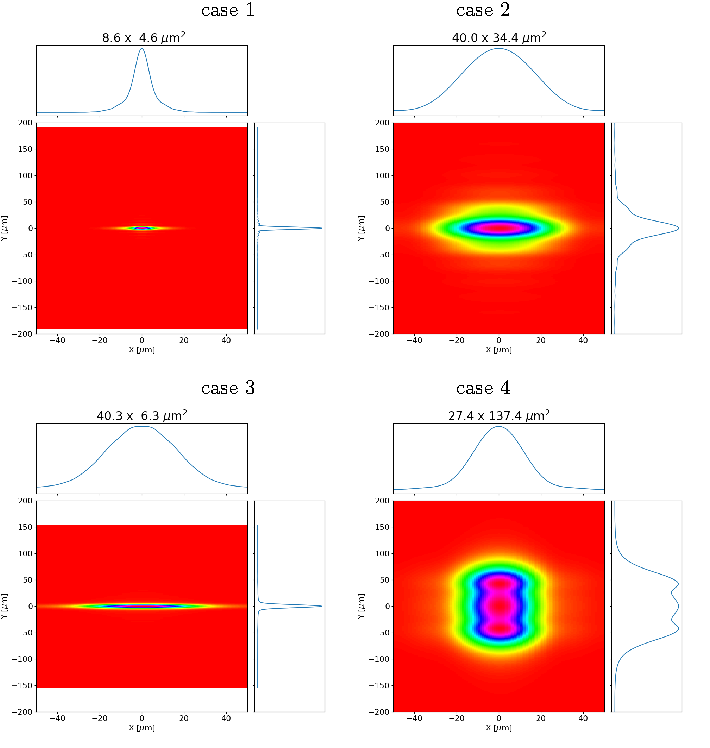
\includegraphics[width=0.99\textwidth]{figures/fig_srw.pdf}
%     \caption{Multi-electron SRW calculations of the intensity distribution at the focal plane for the cases listed in Table~\ref{table:2Dusercases}.}
% \end{figure}


% \begin{figure}\label{fig:comsyl}
%     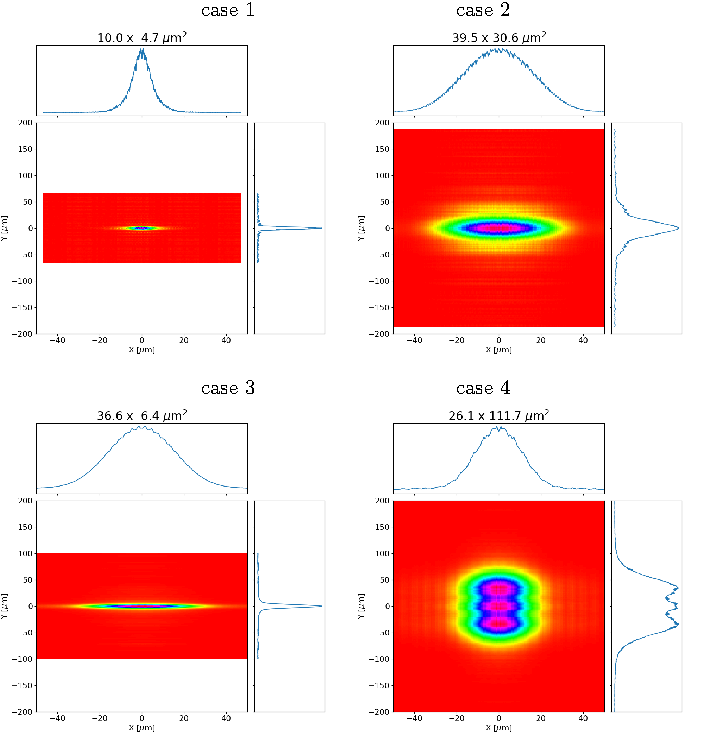
\includegraphics[width=0.99\textwidth]{figures/fig_comsyl.pdf}
%     \caption{COMSYL calculations of the intensity distribution at the focal plane for the cases listed in Table~\ref{table:2Dusercases}.
%     }
% \end{figure}


% \begin{figure}\label{fig:2DWofry1D}
%     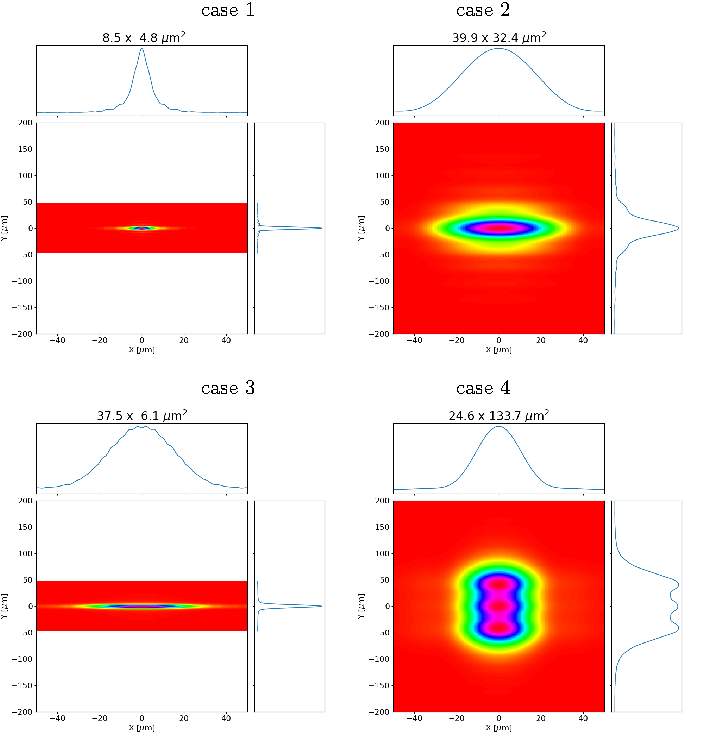
\includegraphics[width=0.99\textwidth]{figures/fig_wofry.pdf}
%     \caption{2D intensity distribution at the focal plane. It has been constructed from the Wofry1D calculations.
%     }
% \end{figure}


% \vspace{1cm}




% \newpage



% \begin{table}[]
%     \label{table:comparison}
%     \caption{Comparison of sizes (FWHM, in \SI{}{\micro\meter}) calculated with different methods for the cases defined in Table~\ref{table:2Dusercases}.
%     In brackets, the values for the fully coherent beam (single electron with SRW, first coherent mode with COMSYL/WOFRY), and zero emittance with Hybrid). \todo{flip columns}
%     }
%     \centering
%     \begin{tabular}{p{0.05\textwidth}|c|c|c|c|c}
%          case h/v &
%          Wofry1D&
%          COMSYL&
%          SRW&
%          Hybrid \\
%          \hline
% 1 h  & 8.5(8.1)    & 10.0 (9.9)  & 8.6 (7.5)   & 17.3 (17.5) \\
% 1 v  & 4.8(4.8)    & 4.7 (5.1)   & 4.6 (4.6)   & 3.3 (3.1) \\
% \hline
% 2 h  & 39.9(38.2)  & 39.5 (39.5) & 40.0 (36.1)  & 39.9 (37.5) \\
% 2 v  & 32.4(29.6)  & 30.6 (29.3) & 34.4 (29.6)  & 74.0 (75.3) \\
% \hline
% 3 h  & 37.5(29.0)  & 36.6 (28.1) & 40.3 (28.4)  & 43.3 (33.0) \\
% 3 v  & 6.1 (4.9)   & 6.4 (5.7)   & 6.3 (4.6)    & 6.5 (5.8) \\
% \hline
% 4 h  & 24.6(19.1)  & 26.1 (18.6)  & 27.4 (18.0)   & 27.1 (18.8) \\
% 4 v  & 133.7(110.3)& 111.7 (90.4) & 137.4 (132.0) & 150.2 (159.8) \\
%     \end{tabular}
% \end{table}

% Hybrid ray-tracing for the four cases defined in Table~\ref{table:2Dusercases} are shown in  Fig.~\ref{fig:hybrid}. One can observe that the intensity distributions as not as structured as for the wave-optics methods (e.g. the three-lobe plateau in case 4v is not reproduced). Values of FWHM are in consonance with full wave-optics calculations for most cases (with the exception of two particular cases:
% 1h (hybrid \SI{16.5}{\micro\meter} Wofry1D \SI{8.5}{\micro\meter}),
% 2v (\SI{71.2}{\micro\meter} Wofry1D \SI{32.4}{\micro\meter}). They will be discussed in the next section.


% SRW-ME results for the four cases are shown in Fig.~\ref{fig:srw}. The good convergence of the values displayed is guarantee by a convergence analysis described in Appendix~\ref{appendix:srw}.
% It was used to determine the minimum number of electrons that produce accurate results. The SRW-ME simulations for the cases analyzed converge with only a few thousands electrons, that can be run in less than one hour in a node with 28 CPUs totalizing 256 GB. The reason is that the beam after the slit has a relatively high CF. 


% COMSYL requires high performance computing (HPC) to perform full CMD of undulator beam, by
% solving the Friedholm problem and obtain the full 2D eigenfunctions (coherent modes) and eigenvalues.
% Simulation of the source with COMSYL took 55 min using 28 x 3.30 GHz CPUs of 251.82 GB RAM, for getting 174 modes of 1691 $\times$ 563 pixels.
% The modes calculated by COMSYL are loaded in the OASYS environment \cite{codeOASYS} to propagate the modes along the beamline.
% The propagation uses 2D zoom propagator and the optical elements available in WOFRY. Results are shown in Fig.~\ref{fig:comsyl}. 
% The beam profiles calculated with COMSYL are a bit noisy, which could be improved by increasing the source sampling and further optimizing the propagation parameters. 


% WOFRY 1D results are shown in Fig.~\ref{fig:2DWofry1D}. The 1D intensity profile for one direction is obtained from the summation of several modes. High modes have very low eigenvalue and it is enough to consider only 10 modes for reproducing more that 99\% of the spectral density. The 2D intensity distribution shown in Fig.~\ref{fig:2DWofry1D} is obtained combinin the calculated horizontal and vertical 1D profiles via the outer product. We can observe in the intensity distributions the same structures due to the diffraction effects than were observed with the other calculation methods. 
% The agreement between the results of  Wofry1D (Fig.~\ref{fig:2DWofry1D}) with SRW (Fig.~\ref{fig:srw}) is striking. All intensity distributions reproduce exactly the same features, and the FWHM values are different in less than 12\%, a value that is compatible with the errors of the simulations (discussed in section~\ref{sec:discussion}). This results validates the 1D CMD method proposed here, whose requirements in computer power are extremely low (it runs very fast in an averaged laptop).  

% The specific numeric value for sizes calculated with the different methods (Table~\ref{table:comparison}) depends not only on the code itself, but also on the particular specific parameters in each method (number of pixels for sampling wavefronts, propagation parameters, etc.). To estimate the calculation error in the final size numbers, we vary randomly these specific parameters in a reasonable range (e.g., 10\%). The evaluation of the mean size and the dispersion (standard deviation) of the sizes obtained give an good estimation of the error in this parameter. This exercise would take a considerable computational effort using 2D methods, but it can be easily done with Wofry1D. We run 200 cases with 10\% random variation in the values in number of pixels and magnification factor in drift spaces. The obtained sizes (horizontal $\times$ vertical) are  
% 8.49 $\pm$ 0.60 $\times$ 4.97 $\pm$ 0.37 \SI{}{\micro\meter}$^2$ (case 1),
% 39.94 $\pm$ 2.98 $\times$ 32.77 $\pm$ 2.69 \SI{}{\micro\meter}$^2$ (case 2),
% 36.39 $\pm$ 2.89 $\times$ 6.12 $\pm$ 0.51 \SI{}{\micro\meter}$^2$ (case 3), and
% 24.18 $\pm$ 1.80 $\times$ 133.44 $\pm$ 10.06 \SI{}{\micro\meter}$^2$ (case 4). We confirmed that the values given in Fig.~\ref{fig:2DWofry1D} are within these error intervals.


% The calculated beam sizes should be completed with flux. At \SI{7}{keV}, the undulator in the configuration selected emits a flux of 1.5 10$^{15}$ photons/s/0.1\%bw. Each of the three elements studied (slit, lens -1 and lens-2) absorb part of the flux. The estimation of the absorption by the slit can be done using simple geometrical arguments, and the absorption by the slits depend on the average Be thickness presented to the beam. The linear attenuation coefficient of Be at 7 keV is $\mu=$~\SI{3}{\centi\meter}$^{-1}$, giving 1.45\% attenuation for a \SI{50}{\micro\meter} thick layer (like lens thickness used in simulations\footnote{In the simulations the horizontal and vertical focusing are separated in two lenses, with accumulated thickness \SI{100}{\micro\meter} thus absorption 3\%}). For the case 1 simulations we extracted the absorption for the different absorbing elements (slit, lens-1 and lens-2) in the case of partial coherence and also for full coherence (see Table~\ref{table:absorption}).
% There is excellent agreement for partial coherence. For full coherence, the Wofry1D results are different than the SRW+Hybrid, because the geometry of the 1st coherent mode used to represent the full coherent beam is not the same as the geometry of the filament beam (used in SRW and Hybrid). We note a high absorption in lens-2, due to the fact that in this case the lens-2 is overilluminated, therefore the \SI{1}{\milli\meter} physical aperture absorbs considerably the beam.

% \begin{table}[]
%     \label{table:absorption}
%     \caption{Comparison of beam intensity attenuation in percent by the slit, lens-1 and lens-2 for the partial coherent beam, 
%     % coherent beam (first coherent mode in Wofry1D, filament beam in SRW, zero emittance in Hybrid) and for the partial coherent beam,
%     for the four cases studied.
%     The Wofry1D data shown here comes after combining the horizontal and vertical wavefronts using the outer product. 
%     }
%     \centering
% \begin{tabular}{l|lll|lll|lll}
% case & \multicolumn{3}{c|}{slit} & \multicolumn{3}{c|}{lens-1} & \multicolumn{3}{c|}{lens-2} \\
% \hline
%      & \rot{Wofry1D} & \rot{SRW} & \rot{Hybrid}
%      & \rot{Wofry1D} & \rot{SRW} & \rot{Hybrid}
%      & \rot{Wofry1D} & \rot{SRW} & \rot{Hybrid}
% \\
% \hline
% %    &          &      &        &          &      &         &          &       &         \\
% %1      &   87.0   & 96.6 & 96.7   & 7.6      & 7.4  & 5.2     & 48.3     & 51.3  & 53.0   \\
% 1       &   97.6   & 97.6 & 97.2   & 7.9      & 7.6  & 5.2     & 50.7     & 51.1  & 52.6   \\
% % 2c    &   87.0   & 96.6 & 96.7   & 6.7      & 6.4  & 4.3     & 3.8      & 3.7   & 3.3    \\
% 2       &   97.6   & 97.6 & 97.2   & 7.0      & 6.6  & 4.3     & 3.9      & 3.7   & 3.3    \\
% % 3c    &   55.9   & 86.0 & 85.6   & 5.4      & 6.11 & 4.7     & 17.1     & 22.7  & 26.6   \\
% 3       &   89.5   & 90.2 & 88.6   & 6.3      & 6.1  & 4.6     & 23.4     & 21.8  & 25.2   \\
% % 4c    &   55.9   & 86.0 & 85.6   & 6.8      & 7.73 & 6.4     & 3.6      & 3.6   & 3.6    \\
% 4       &   89.5   & 90.2 & 88.6   & 8.0      & 7.7  & 6.2     & 3.8      & 3.6  & 3.6   \\
% \end{tabular}
% \end{table}


% \section{Discussion}
% \label{sec:discussion}

% % Our discussion follows a hierarchical approach, as discussed in \citeasnoun{hierarchical}, with the idea of balancing accuracy and computational effort, to subsequently select and use the most advantageous method for the analyzed problem. 
% % This multi-method analysis will also help to validate the new 1D CMD method introduced in this work. The results of the Wofry1D results are compared with other well-known simulation packages. 


% There is good agreement in focal size FWHM values in all methods (see Table~\ref{table:comparison}), but also in the shape of intensity distributions, in particular for the wave optics methods (compare Figs. ~\ref{fig:2DWofry1D}, ~\ref{fig:comsyl} and ~\ref{fig:srw}). 

% Regarding computer resources, the Wofry1D code can be run in a few seconds in a laptop, whereas the simulation of the full CMD with COMSYL required about 1h (for 1691 x 563 pixels, 174 modes) using 1 node of 28 cores. This source is then reused for propagating the different configurations. Each configuration required a full SRW-ME with 5000 electrons run in also about 1h in a similar configuration. 

% \todo{a possible paragraph discussing surface errors. Just to show it as a proof of concept: FEM at the white mirror, slope error at the mirros, FEM at the monochromator... Cons: it will be done with only Wofry1D (too much work for the full collection of codes); the results will not change what we have}


% \todo{A possible discussion of the Gaussian Shell-model. I am not much in favor of including the GSM here, but it can be done. Main points for the discussion:

% \begin{itemize}
% \item Discuss how to match the GSM with undulator parameters: there are several possibilities... I prefer matching the size and CF. 
% \item Compare Hermite-Gaussian modes with numerical modes. There are similar nut not identical. For incoherent sources the GSM may be a good approximation, for pretty coherent sources not. 
% \item Show that propagation of GSM modes is very different than propagating undulator modes. Indeed, because $\sigma \sigma' = \lambda / (4 \pi)$ in GSM and with $2\pi$ in undulator either the size at the source or the propagated size is wrong with GSM.
% \item Analytical propagation of the modes (as described by Vartanyants et al.) only works for ideal elements, and Gaussian slits. They fail in simulating structures like those that we obtain, because they are originated by the slit, which is non-Gaussian.
% \end{itemize}

% }






% % \subsection{Hybrid ray-tracing}

% % The simulation results for the four cases studied using the hybrid method indicate that, although this method does not reproduce exactly the intensity distibution given by full partial coherent optics, the numerical values are approaching the good ones, but with two exceptions: the case 
% % 1h (hybrid \SI{16.5}{\micro\meter} Wofry1D \SI{8.5}{\micro\meter}) and the case 
% % 2v (\SI{71.2}{\micro\meter} Wofry1D \SI{32.4}{\micro\meter}). 
% % We remark that these thee cases have in common that the $f_1$ value in use is close to $f_1$~=~\SI{40}{\meter} that corresponds to the singularity in the analytical (geometrical optics) calculations, when the lens-1 focuses on lens-2. A detailed study with hybrid was performed to calculate the FWHM for all possible values of $f_1$ (as done in Fig.~\ref{fig:focalSizes}. The result (Fig.~\ref{fig:focalSizes_hybrid}) confirms that there is good agreement everywhere except in the region close to $f_1$~=~\SI{40}{\micro\meter}.
% % We thus conclude that the hybrid ray-tracing is a valid method to obtain good values of focal sizes in most cases, excepts for the case that lens-1 focus is close to the position of lens-2 ($f_1 \approx $~\SI{40}{\meter}).


% % \begin{figure}
% %     \centering

% %     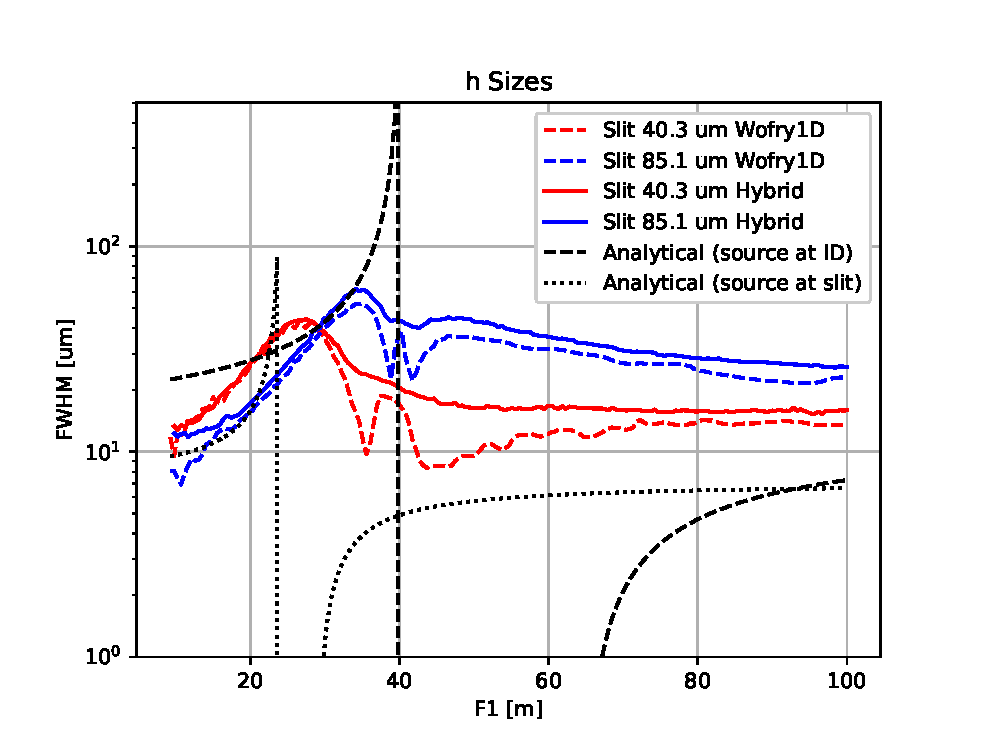
\includegraphics[width=0.95\textwidth]{figures/sizes_h_hybrid.eps}
% %     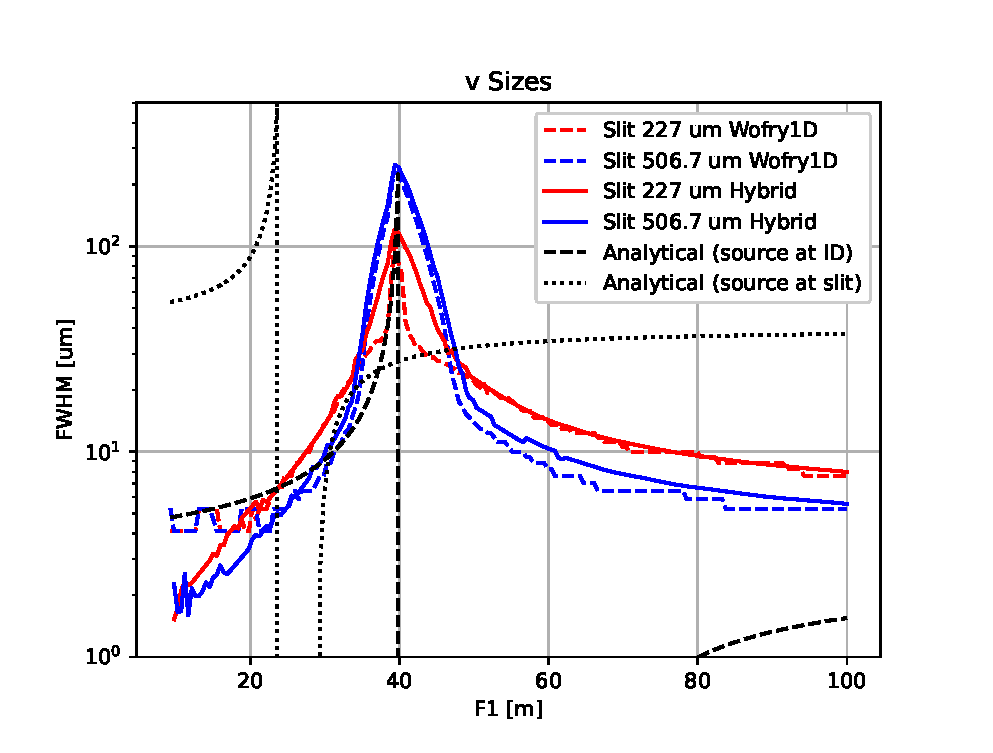
\includegraphics[width=0.95\textwidth]{figures/sizes_v_hybrid.eps}
        
% %     \caption{Focal sizes obtained by hybrid ray-tracing method, for two slit aperture cases, compared with values from Wofry1D  (from Fig.~\ref{fig:focalSizes}).}
% %     \label{fig:focalSizes_hybrid}
% % \end{figure}

% % \subsection{Further simulations}

% The simulations presented, motivated by the ID18 project, use a simplified optical layout. A more complete study including the other optical elements, other transfocator configurations will be presented elsewhere, also for different energies and implementing the effect of surface errors due to thermal load and surface finish. 

% % We have also calculated the beam evolution in the neighbourhood of the sample position for the four cases studied (see Fig.~\ref{fig:caustic}). From these plots one can obtain the position of the best focus and the depth of focus. The depth of focus (measured as the distance where the peak value is reduced by 15\%) is larger than two meters (except for the cases 1v, 3v). \todo{redo these plots and compare with SRW... otherwise supress?}

% % In some cases there is a mismatch between the position of the best focus and its expected position (the sample position, at the zero abscissas). This effect, certainly due to an error in setting $f_2$, may have several origins. 

% % For pairing two transfocators, the algorithm chosen to calculate the $f_2$ value consist in analyzing the wavefront at the lens-2 position, find a corrector refractive object that would transform the incoming wavefront in a converging wavefront (see section \ref{sec:refractorCorrector}), and fit the radius at the center. We then get the $R_2$ and therefore the $f_2$ value. In addition, to obtain smooth $(f_1,f_2)$ curves in Fig.~\ref{fig:f1f2map} we have used a Gaussian slit (see section \ref{sec:gaussianslit}). It smears out the diffraction fringes, because in an ideallized system where a point source is focused at the sample position, the recorded intensity would correspond to the diffraction pattern of the slit, that can be considered as an "object" placed in the beam (see e.g. \cite{paganin_book}). The use of a Gaussian object implies that its diffraction pattern is a Gaussian with no diffraction fringes. 

% % For cases 1h, 1v, 3v (see  Fig.~\ref{fig:caustic}), there is a good agreement between the focal position obtained from the maximum of intensity on-axis (plotted at the top of the image) and our expected position (the zero in the plots). In some other cases (2v, 3h, 4h) the agreement is acceptable, taking into account that the observed depth of focus is of the order of meters. A small correction in $f_2$ would bring the best focus to its ideal position. This correction is necessary because we used a Gaussian slit for calculating $f_2$, thus neglecting some oscillations around the $(f_1,f_2)$ curves. There are two pathological cases where the algorithm used to calculate $f_2$ did not succeed: the cases 2h and 4v.
% % The error in $f_2$  for case 2h is also due to the oscillations in the $(f_1,f_2)$ and can be corrected, as shown in Fig.~\ref{fig:causticcorrection}a. However, case 4v cannot be corrected because we would need a divergent lens to bring the focus of $f_1$ to the sample position. Setting $R_2=f_2=\infty$ would reduce the beam size at the sample position (Fig.~\ref{fig:causticcorrection}b), but cannot get the best focus there. However, an ad-hoc defined refractive corrector in the place of lens-2 would do the job (Fig.~\ref{fig:causticcorrection}d).  

 



% %%%%%%%%%%%%%%%%%%%%%%%%%%%%%%%%%%%%%%%%%%%

% % \begin{figure}\label{fig:caustic}
% % \centering

% % 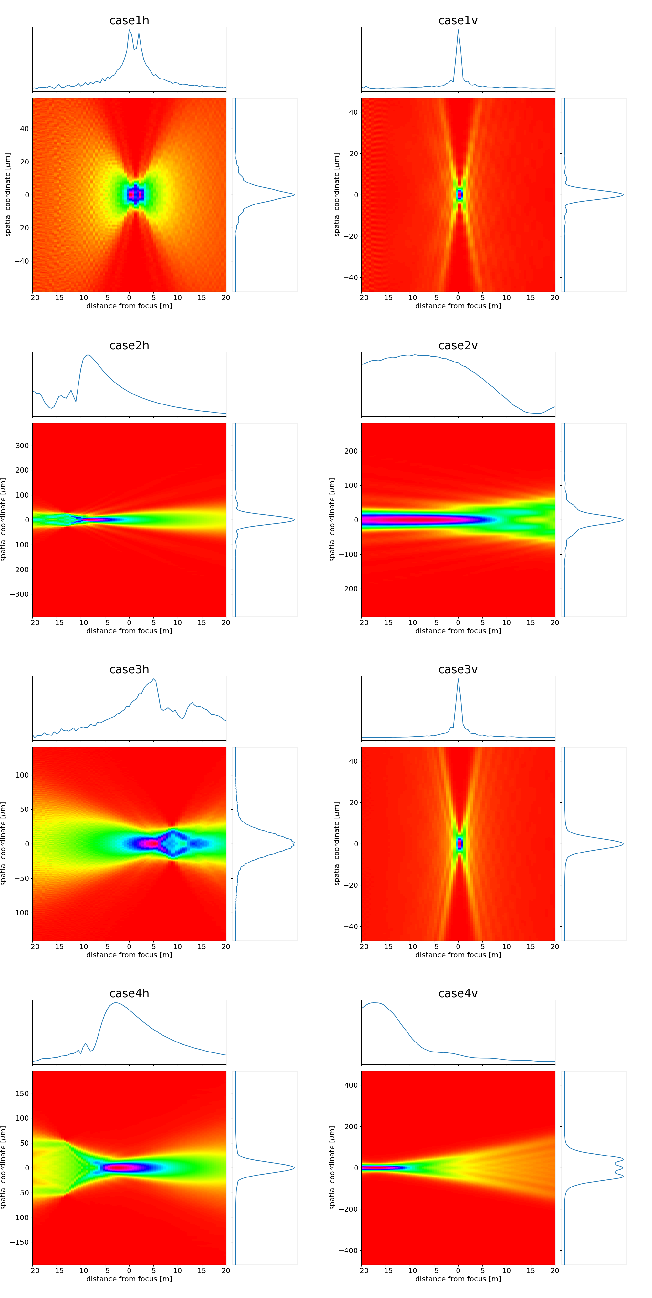
\includegraphics[width=0.99\textwidth]{figures/fig_caustic.pdf}

% % \caption{Evolution of the beam size in the around the sample position for the cases listed in Table~\ref{table:2Dusercases}. The top and side graphs correspond to the profiles passing by (0,0).
% % }
% % \end{figure}



% % \begin{figure}\label{fig:causticcorrection}
% % \centering
% % 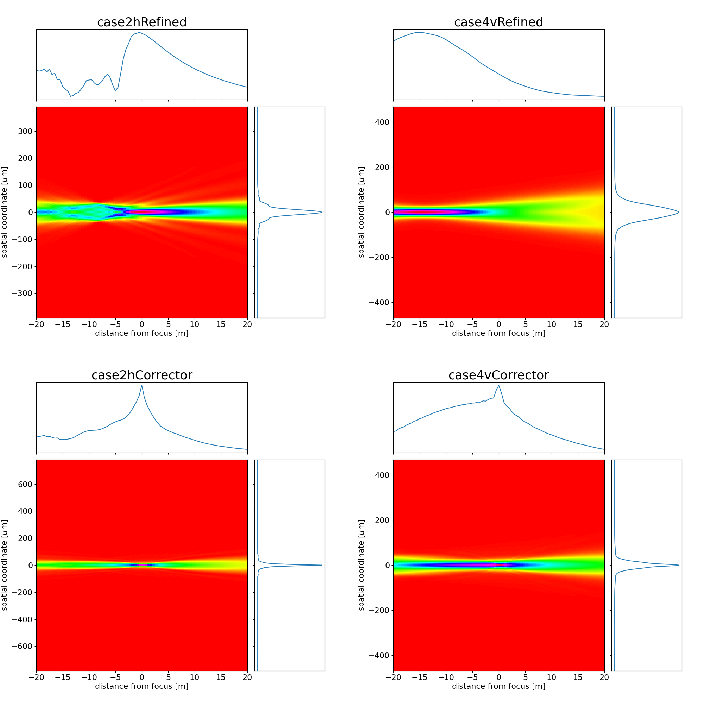
\includegraphics[width=0.99\textwidth]{figures/fig_caustic_correction.pdf}

% % \caption{Evolution of the beam size in the around the sample position for the ``pathological" case 2h and 4v shown in Fig.~\ref{fig:caustic}. Top row: using corrected lens-2 with $R_2$=\SI{410}{\micro\meter} ($f_2=$\SI{29.4}{\meter}) for case 2h and $R_2=f_2=\infty$ for case 4v. Bottom: using a free-form refractive corrector instead of lens-2.
% % }
% % \end{figure}


% % \subsection{Errors in optical surfaces}

% % % \todo{Rafael, please re-read}
% % The performance of X-ray optics in the new generation synchrotron beamlines is limited by the quality of the optical surfaces \cite{lengeler1999,Yabashi}. Finish errors can be divided in three families: i) height errors, associated with surface finishing (high spatial frequency), ii) figure errors, associated with deviations from ideal profile (e.g. bending, gravity sag, thermal deformations), and iii) slope errors or waviness, associated to medium spatial frequencies \cite{srio1992, signorato1997}. Finish errors in x-ray lenses can be measured by different techniques (eg. grating interferometry, x-ray speckle tracking or ptychography) and readily included in the simulations \cite{Celestre:mo5214}. Some profiles measured at ESRF using x-ray speckle tracking \cite{berujon2020} with height error RMS of the order of \SI{1}{\micro\meter} are used to verify that the focal spot produced by lenses with realistic errors is not degraded with respect to the ideal lens surface. 

% % Usually the optics of new generation synchrotron beamlines is limited by the quality of the optical surface. Typically are due to surface finish (slope errors and height errors) and shape errors, often due to heat load. 
% % \todo{Rafael, would you please work next paragraph. I checked that your error file (profile 1 in DABAM2D) does not produce relevant changes, thus the idea is to "mention" the errors without presenting a full study.} Surface errors in lens surfaces can be experimentally measured by different techniques (e.g. speckle tracking, ptychography) and included in the simulations. Some profiles measured at ESRF \cite{???} with height error RMS of the order of \SI{1}{\micro\meter}  are used to verify that the focal spot produced by lenses with realistic errors is not degraded with respect to the ideal lens surface. 

% % The effect of finish errors in the white double-mirror system is also analyzed using a measured mirror meridional profile of \SI{2.5}{\nano\meter} height error RMS and \SI{140}{\nano\radian} RMS slope error. 

% % % \todo{Philipp, please re-read}
% % The heat load affect several elements of the beamline. For the beamline under consideration, the affected elements (white beam mirrors, and double-crystal monochromators) are not presented in our simulations. Finite element analysis of mirrors and crystals done for other EBS beamlines \cite{Brumund} show that the deformation height profile can be decomposed it two parts: an average bending that is possible to correct by a small readjustment of the focal length of the optical elements downstream the heated element, and a ``residual error" which remain after removing the averaged bending radius, and could only be corrected using adaptive optics. Wofry1D simulations using FEA-generated deformations at the first crystal of a monochromator placed just after the coherent slit showed no significant degradation of the focal spot, both in size and shape. This is mainly due to the low power transmitted by the coherent slit. We checked that the focused beam is almost unchanged when using a profile from FEA analysis with curvature of about \SI{1}{\kilo\meter} and residual slope errors of \SI{30}{\nano\radian}. 



% % The deformation profile calculated by FEA \todo{I USED FILE: SRC\_Si\_3.0mrad\_08000eV\_mo\_Si111\_Size1\_nodalOut.out} is is loaded in a ``mirror-like" element in Wofry, as described \cite{srioLBL}. For case 1, a small degradation in the horizontal direction is found (passing from \SI{8.09}{\micro\meter} to \SI{10.21}{\micro\meter} for the first coherent mode). It is accompanied by a loss of symmetry. A large deformation in the vertical spot is observed, but a spot close to the ideal is found when a best circle is subtracted from the profile. It is then possible to correct this added curvature. Indeed, by adjusting $f_2$ \todo{I will calculate this} it is possible to compensate the effects introduced by the crystal bending due to heat load.


% % finding focus https://www.optikos.com/finding-focus/

% % \subsection{Practical considerations} Simulations like those presented here could be very beneficial for beamline operation, for its optimization and quick setting.  Complicated  relationships exist between the beam parameters requested by users (beam size and coherent fraction) and the beamline configuration (undulator, slit and transfocator setting). Quick simulations as done by Wofry1D could be a helpful instrument for the beamline staff to get the desired configurations. The plots shown here (e.g., $CF$ vs slit size in Fig.~\ref{fig:cf_vs_aperture}, trajectories in Fig.~\ref{fig:f1f2map}, or final size in Fig.~\ref{fig:focalSizes} could be simulated on-line and compared with results presented as look-up tables with similar aspect. We are also considering the design of a digital twin that mimics the real transfocator systems to assist beamline setting. For that, the fast simulation using the CMD method developed in Wofry1D will be an integrated component.  

% % Some practical consequences can be directly deduced from the results shown here. For example, looking at Fig.~\ref{fig:focalSizes} one can observe that the same focal size can be obtained with different configurations. To get a similar size, it is better to prefer a large $f_1$ to avoid over-illuminating the lens-2 and increase transmission of lens-1. The transfocator design is simplified if we restrict the horizontal focal distance t to be smaller than the vertical $f_h>f_v$. Here, $f_v$ can be obtained with lenses focusing in 2D and $f_h$ by adding 1D lenses focusing in the horizontal plane. 

% % % https://www.optikos.com/finding-focus/
% % In this work we configured the transfocator to have the resulting focal position on the sample plane, an "in-focus" setup. It could also be possible to work off-focus to vary the beam size at the sample plane. The in-focus setup will generally produce the sharpest image of very small details in the image. Moreover, it will reduce the artifacts produced by the surface finish errors. Also, a larger depth of focus is obtained at this position (see e.g. Fig.~\ref{fig:causticcorrection}).


% \section{Summary and conclusions}
% \label{sec:summary}

% We have studied a particular case of focusing a partial coherent beam (as produced by the low emittance storage ring EBS-ESRF) by a system of two transfocators (or lenses). We have verified that four simulation codes typically used to simulate synchrotron beamlines agree in the results of beam size and flux. The hybrid ray-tracing method (ShadowOUI) fails to determine fine structures in the beam intensity profiles. The three codes using physical optics (SRW-ME, COMSYL and WOFRY1D) produce essentiually the same results. Partial coherence calculations using 2D wavefronts are expensive from the computation point of view, either because many thousands of wavefronts are propagated (in SRW-ME) or because the need of diagonalizing an extremely large 4D cross spectral function. The newly developed coherent mode decomposition of 2D CSFs (i.e. separating 1D modes for the horizontal and vertical direction) is very rapid and can be run interactively in a laptop. Its results for the particular cases simulated here agree very well with full 2D propagation methods. 
% This method is available in the Wofry add-on of the OASYS suite \cite{codeOASYS}. OASYS workspaces for the simulations performed in this paper are available\footnote{{ https://github.com/oasys-esrf-kit/paper-multioptics-resources}}.

% % Four cases are calculated and compared using the other methods available in OASYS, like the full 2D coherent mode decomposition using COMSYL \cite{codeCOMSYL}, the OASYS interface for the SRW \cite{codeSRW} code, and hybrid ray-tracing \cite{codeHYBRID}.


% %%%%%%%%%%%%%%%%%%%%%%%%%%%%%%%%%%%%%%%%%%%%%%%%
% %%%%%%%%%%%%%%%%%%%%%%%%%%%%%%%%%%%%%%%%%%%%%%%%
% %%%%%%%%%%%%%%%%%%%%%%%%%%%%%%%%%%%%%%%%%%%%%%%%
% \appendix

% \section{Some considerations on partially-coherent calculations using SRW's macro-electrons \& simulation convergence}
% \label{appendix:srw}

% The convergence of the SRW-ME method is based on the \textit{finesse} with which the distribution $f(\textbf{s}_\text{e}, \textbf{s}'_\text{e}, \gamma_\text{e})$  in equation~(\ref{eq:SR}) is sampled. While an exquisitely large number of \textit{me's} will lead to a more accurate simulation, the resulting calculation would be very long and impossible to be performed on personal computers within reasonable time even if performed in parallel. The number of \textit{me's} depends on overall beamline degree of coherence at the observation plane, which is impacted by the source coherent fraction and beamline overall transmission (eg. slits, creation of secondary sources or any other spatial filtering scheme). Special attention to the number of macro-electrons should be given if the simulation accounts for vibrations in the beamline elements or broad-band radiation (eg. pink beam or radiation filtered by multi-layer monochromators).

% To illustrate the effect of the number of macro-electrons on the beam profile we choose the previously studied cases 1 and 3 from section~\ref{sec:complete-beamline} - due to their $CF$, cases 2 and 4 are expected to have the same convergence as 1 and 3, respectively. Both systems 1 \& 3 (and 2 \& 4) have the same X-ray source and are illuminated up until the slits (36~m downstream U18) by the same beam, differing mainly by the coherent fraction selected for the rest of the beamline with case 1 having a higher $CF$ than case 3 - refer to Tables~\ref{table:id18parameters} and \ref{table:2Dusercases} for the complete simulation parameters. The results for a selected number of \textit{me's} are shown in Figs.~\ref{fig:me_c1} and \ref{fig:me_c3}. The 1 \textit{me} simulation represents the filament-beam source, where the electron beam emittance is negligible and the fully spatial coherence is assumed - this is often called a ``single electron simulation". On the other extreme, an exaggerated value of 100k $me's$ is chosen as a way of guaranteeing convergence by brutal-force. Two criteria are used to evaluate the convergence of the simulations: the beam shape and peak intensity stabilisation. The profile cuts in  Fig.~\ref{fig:me_c1}(a)-(b) and Fig.~\ref{fig:me_c3}(a)-(b) show that the profile shape starts to converge to that of a 100k $me's$ after $\sim$500 macroelectrons for case 1 and $\sim$1k macroelectrons for case 3. Beyond that, it is necessary to resort to the relative error standard deviation and the peak intensity stabilisation. Fig.~\ref{fig:me_c1}(c)-(d) and Fig.~\ref{fig:me_c3}(c)-(d) show that for both cases, the convergence happens between 2k and 5k $me's$. Further increase in the number of macro electrons does not translate in improvements in the simulations (see simulations for 10k $me's$ onward), but increase greatly the cost of the calculation as shown in Fig.~\ref{fig:me_t}. For the work presented here a good compromise between accuracy and efficiency of the calculations is reached at 5k $me's$. Other factors contributing to the total elapsed simulation time and overall parallel performance of SRW-ME method are presented in \S3.3 from \cite{codeSRW_MEscan}, but these do not impact the SRW-ME convergence.

% It is important to note that this large scan procedure is merely illustrative. Usually an experienced optical designer starts with a good guess of the necessary number of $me's$ based on the characteristics of the source (degree of coherence) and optical system (transmission and expected degree of coherence at the observation plane). This choice usually includes considerations of time and resources consumption. If there are signs that the choice may be too low, further attempts with higher $me's$ should be done. If the simulation looks fine from the first guess, reducing the number of $me's$ is also interesting as very often it is necessary to repeat the simulations (eg. testing different configurations, different energies, tolerancing or even different observation planes). At the time of writing, the authors are unaware of any widespread metric within the SRW's community capable of giving the exact number of \textit{me's} necessary for the convergence of the SRW-ME method other than the $me's$ scan. We welcome the discussion on SRW-ME convergence and we encourage the reader to reach out if they employ any interesting and reproducible convergence metric that is less time (and resource) consuming.

% % \begin{table}[]
% % \label{table:me_t}
% % \caption{Time}
% % \resizebox{\textwidth}{!}{
% % \begin{tabular}{cccccccc}
% %  & 500 & 1k & 2k & 5k & 10k & 25k & 100k \\ \hline
% % case 1: & 5min & 9min & 15min & 39min & 1h20min & 3h21min & 13h15min \\
% % case 3: & 9min & 17min & 30min & 1h15min & 2h35min & 6h30min & 35h39min
% % \end{tabular}}
% % \end{table}

% \begin{figure}
%     \centering
%     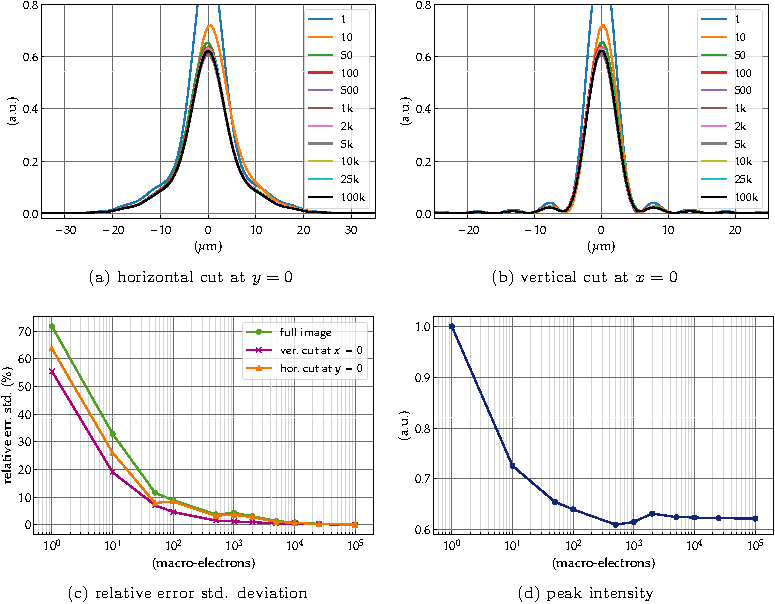
\includegraphics[width=\textwidth]{figures/c1.pdf}
%     \caption{Partially-coherent simulations convergence study: case 1. (a) horizontal and (b) vertical intensity cuts at E=7~keV for $me's$ ranging from 1 to 100k. (c) errors relative to the $me's=$100k plots and (d) peak intensity.}
%     \label{fig:me_c1}
% \end{figure}

% \begin{figure}
%     \centering
%     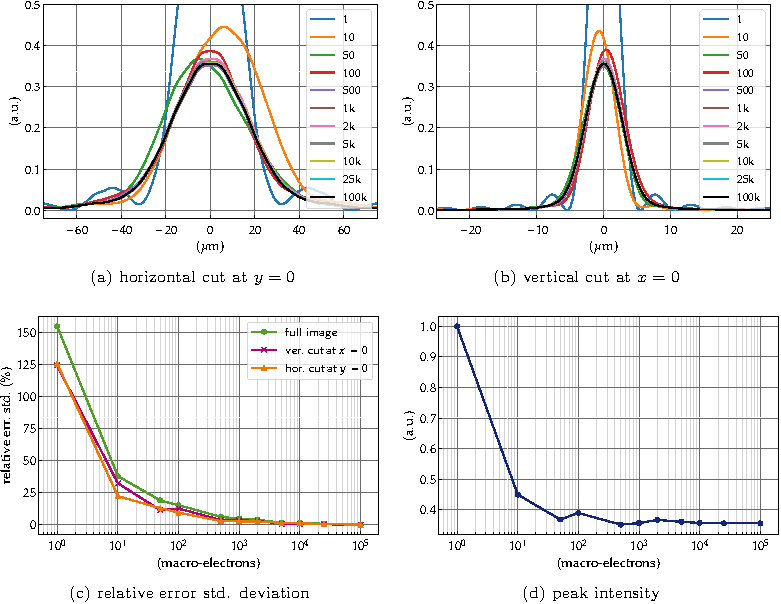
\includegraphics[width=\textwidth]{figures/c3.pdf}
%     \caption{Partially-coherent simulations convergence study: case 3. (a) horizontal and (b) vertical intensity cuts at E=7~keV for $me's$ ranging from 1 to 100k. (c) errors relative to the $me's=$100k plots and (d) peak intensity.}
%     \label{fig:me_c3}
% \end{figure}

% \begin{figure}
%     \centering
%     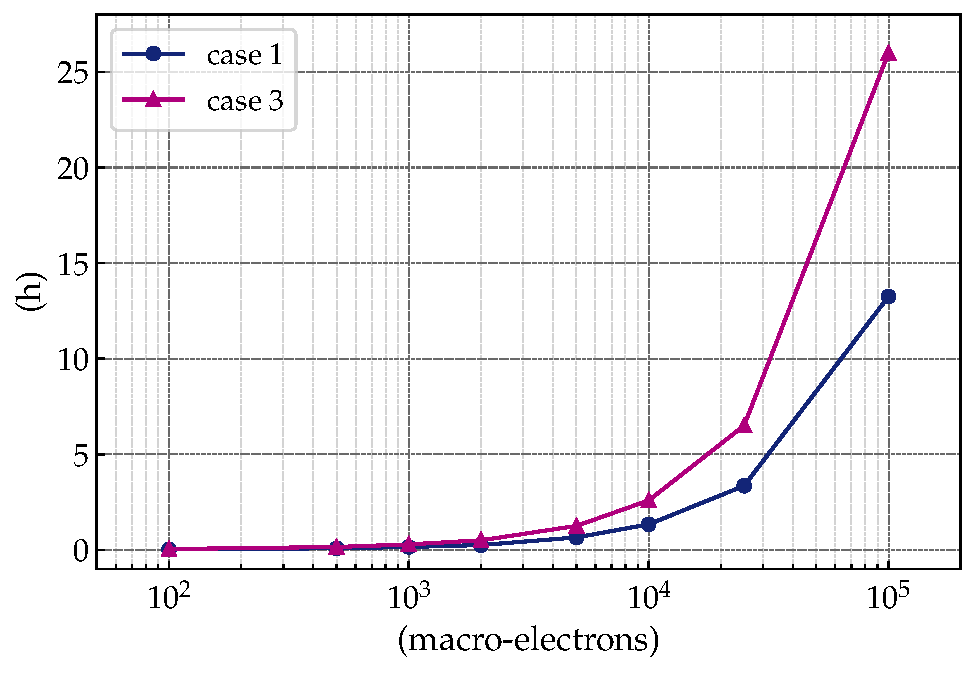
\includegraphics[width=0.8\textwidth]{figures/srw_time.pdf}
%     \caption{Total elapsed time for partially-coherent simulations using a computer cluster with 28 processors for parallel calculations as a function of number of $me's$.}
%     \label{fig:me_t}
% \end{figure}

% \newpage
% % %%%%%%%%%%%%%%%%%%%%%%%%%%%%%%%%%%%%%%%%%%%%%%%%
% % %%%%%%%%%%%%%%%%%%%%%%%%%%%%%%%%%%%%%%%%%%%%%%%%
% % %%%%%%%%%%%%%%%%%%%%%%%%%%%%%%%%%%%%%%%%%%%%%%%%

%  %-------------------------------------------------------------------------
%  % The back matter of the paper - acknowledgements and references
%  %-------------------------------------------------------------------------

%  % Acknowledgements come after the appendices

% \ack{\textbf{Acknowledgements}}

% This project has received funding from the European Union’s Horizon 2020 Research and Innovation programme under grant agreements N$^{\circ}$ 823852 (Photon and Neutron Open Science Cloud -- PaNOSC) and N$^{\circ}$ 101007417 (NFFA-Europe Pilot Joint Activities -- NEP).
% %. R.C. acknowledges funding from the European Union’s Horizon 2020 research and innovation programme under grant agreement N$^{\circ}$ 101007417 within the framework of the NFFA-Europe Pilot Joint Activities.




\referencelist{iucr}

 %-------------------------------------------------------------------------
 % TABLES AND FIGURES SHOULD BE INSERTED AFTER THE MAIN BODY OF THE TEXT
 %-------------------------------------------------------------------------

     

\end{document}                    % DO NOT DELETE THIS LINE
%%%%%%%%%%%%%%%%%%%%%%%%%%%%%%%%%%%%%%%%%%%%%%%%%%%%%%%%%%%%%%%%%%%%%%%%%%%%%%

